\documentclass[a4paper, 12pt]{report}


\usepackage[utf8]{inputenc}
\usepackage[T1]{fontenc}
\usepackage[spanish]{babel} 
\usepackage{graphicx}
\usepackage{amsmath}
\usepackage{amssymb}
\usepackage{mathtools}
\usepackage{amsthm}
\usepackage{bbm}
%\usepackage[shortlabels]{enumitem}
\usepackage{enumerate}
\usepackage{array,tabularx}
\usepackage{float}
\usepackage{wrapfig}
\usepackage[export]{adjustbox}
\usepackage[rightcaption]{sidecap}
\usepackage{multirow}
\usepackage{subfig}
\usepackage{capt-of}
\usepackage{captdef}
\usepackage{color}
\usepackage{soul}
\usepackage{hyperref}
\usepackage{stmaryrd}
\usepackage{fullpage}
\usepackage{xcolor}
\usepackage{listings}

\newcommand{\Ra}{\Rightarrow}
\newcommand{\ra}{\rightarrow}
\newcommand{\N}{\mathbb{N}}
\newcommand{\R}{\mathbb{R}}
\newcommand{\te}{\text}
\newcommand{\Lra}{\Leftrightarrow}
\newcommand{\lra}{\leftrightarrow}

\theoremstyle{definition}
\newtheorem{ejercicio}{Ejercicio}[section]

\begin{document}

\centerline{\Huge\bf Apuntes de Introducción a la Computación}



\tableofcontents

\chapter{Introducción}

 En este curso planteo a grandes rasgos tres objetivos. El primero es que aprendan las bases de la programación. 
Otro objetivo es que desarrollen la capacidad de utilizar las computadoras con fines matemáticos, como por ejemplo para determinar si un número es primo, o aproximar numéricamente el valor de una integral, o generar gráficas de distintos tipos.
El otro objetivo es que desarrollen la capacidad de entender la computación como un concepto abstracto matemático, para desarrollar programas en base a razonamiento matemático y además poder demostrar matemáticamente propiedades sobre estos programas.
De modo sintético, este curso se trata de programación, de computación para matemática y de matemática para computación.

En este capítulo el objetivo principal es dar una idea básica de qué es la computación, cómo funcionan las computadoras y qué son los lenguajes de programación.



\section{Conceptos básicos de computación e intuiciones}

La computación se trata de operaciones definidas por reglas precisas que operan con objetos finitos y en una cantidad finita de pasos llegan a un resultado.

Los objetos finitos, a los que en general llamaremos {\bf datos}, pueden ser por ejemplo números naturales, palabras o listas finitas. Cabe aclarar que al decir que los números naturales son finitos nos referimos a que cada número natural es un objeto finito. Por supuesto que el conjunto de todos los números naturales, por otra parte, es infinito.

A una operación definida por reglas precisas que opera con datos y termina en finitos pasos le llamaremos {\bf algoritmo}. Un programa es lo mismo que un algoritmo. Un ejemplo de algoritmo es el de la suma que se aprende en la escuela. Dados dos números, aplicando una secuencia finita de pasos bien definida se llega al resultado.


Una buena analogía consta de las recetas de cocina. Sin embargo, hay una diferencia importante. En las recetas de cocina, por la naturaleza de la situación, pueden haber ciertas ambigüedades, o puntos en los que hay que tomar una decisión, de modo que si dos personas realizan la misma receta el resultado puede ser distinto, sin que ninguno de los dos lo haya hecho mal. Pueden haber frases como <<un poquito de sal>> que según la persona se traduzcan a distintas cantidades. En computación, un algoritmo bien ejecutado debe tener un único resultado correcto, como ocurre con la suma. Que las reglas sean precisas significa que no hay margen de variabilidad en lo que se debe hacer, ni puntos en los que un ser con voluntad propia deba pensar y tomar una decisión. Esto es importante por dos motivos. Primero, asegura que si se realiza por una persona, hay un único resultado correcto. Segundo (y tal vez más importante), es necesario para que pueda ser realizado automáticamente por una computadora, que en lugar de un ser con pensamiento y voluntad es una cosa.

Como los algoritmos deben estar bien definidos y no puede haber ninguna ambigüedad, son en esencia conceptos matemáticos. De hecho, la computación teórica es una rama de la matemática.
\subsection{Bases de la formalización matemática}

Una forma de representar algoritmos en computación teórica es mediante funciones $f:\N\to\N$, donde la idea es que si $n$ es la entrada del programa, entonces $f(n)$ es la salida. Como se trata de un algoritmo, no puede ser cualquier función, sino una que puede calcularse en finitos pasos con reglas precisas. A primera vista puede parecer que usar solamente números naturales es una restricción, pero de hecho alcanza para hablar de todo lo que se puede programar. De hecho, dentro de la computadora todos los distintos tipos de datos  se representan con secuencias de bits (\emph{binary digits}, es decir dígitos binarios: 0 o 1) y cualquier secuencia de bits se puede interpretar también como un número escrito en binario. Por lo tanto, todos los datos finitos se pueden representar con números (en general muy grandes). Debido a esto, un programa que recibe como entrada una imagen y retorna la imagen con alguna modificación, por ejemplo, se puede ver como una función $f:\N\to\N$ que recibe el número que codifica la imagen original y retorna el número que codifica la imagen modificada.

Hay distintos formalismos que permiten definir funciones $f:\N\to\N$ computables, es decir, que corresponden a algoritmos. Algunos de ellos son las máquinas de Turing, el cálculo lambda y la teoría de las funciones recursivas. Notablemente, aunque todos son formalismos muy distintos, siempre dan lugar a exactamente el mismo conjunto de funciones computables. Este conjunto de funciones computables no es todo $\N^\N$. De hecho, el conjunto de las funciones computables es numerable, por lo que la mayoría de las funciones no lo son.

Por último, está la pregunta de si la definición matemática de función computable corresponde con las funciones que en el mundo físico se pueden calcular con una computadora. La Tesis de Church-Turing conjetura que efectivamente es el caso. Al ser algo del mundo físico y salirse de la matemática, no hay ninguna prueba formal, pero en general es asumido como cierto.


\section{Arquitectura de Von Neumann}\label{sec-ArqVonNeu}

La arquitectura de Von Neumann es un modelo para computadoras físicas, a diferencia de formalismos como las máquinas de Turing, que son conceptos puramente teóricos.

Primero sería bueno decidir qué consideramos como una computadora. Digamos que es un dispositivo físico que puede automáticamente calcular funciones computables y que tiene mecanismos para interactuar con el entorno. Podemos pensar que es una caja negra que de alguna forma calcula funciones computables y además tiene algún mecanismo por el cual podemos ingresar información (por ejemplo con un teclado) y algún mecanismo por el cual puede devolver información (por ejemplo con una pantalla).

La arquitectura de Von Neumann define que la computadora tiene tres componentes principales que interactúan entre sí: un {\bf procesador }(CPU), una {\bf memoria} y un subsistema de {\bf entrada y salida} (figura \ref{fig-ArqVN}). A la conexión entre las distintas componentes se le llama {\bf bus}. El procesador es un dispositivo con la capacidad de ejecutar un conjunto finito de operaciones básicas, llamadas  instrucciones. La idea es que un programa está dado por una secuencia finita de instrucciones. Si bien las instrucciones son finitas (y en general bastante sencillas), al usarlas de forma secuencial se puede implementar cualquier función computable. Tanto la secuencia de instrucciones que conforma un programa como los datos con los que este opera se guardan en la memoria. El subsistema de entrada y salida permite que la computadora interactúe con el entorno (por ejemplo con un usuario que ingresa datos y observa resultados o con otra computadora dentro de una red).

Todas las componentes de la computadora se construyen con circuitos electrónicos y usando la abstracción del {\sl bit}, que significa dígito binario, es decir {\tt 0} o {\tt 1}. Claramente el bit es un concepto abstracto que no existe de por sí en los circuitos eléctricos. Lo que se hace es tomar una convención, como que si circula corriente significa 1 y si no significa 0, o que cierto voltaje significa 1 y cierto voltaje significa 0. Sea cual sea la convención, lo importante es que se pueden construir circuitos con entrada y salida que implementen cualquier operación finita. Por ejemplo, se puede armar un circuito con 4 bits de entrada, $a_0,a_1,b_0,b_1$ y tres bits de salida $c_0,c_1,c_2$ tal que si tomamos la entrada como la codificación en binario de dos números entre $0$ y $3$, la salida sea la codificación en binario de la suma. En general, para cada función $f:\{0,1\}^n\to\{0,1\}^m$ se puede construir un circuito con $n$ bits de entrada y $m$ bits de salida que implementa la función~$f$. A estos se les llama {\sl circuitos combinatorios}. Junto con otro tipo de circuitos llamados {\sl secuenciales} (que funcionan por etapas y además de la entrada actual dependen de las entradas anteriores, o de un estado que puede ir variando), son un elemento base de las computadoras, tal vez el principal.




\begin{figure}
	\centering
	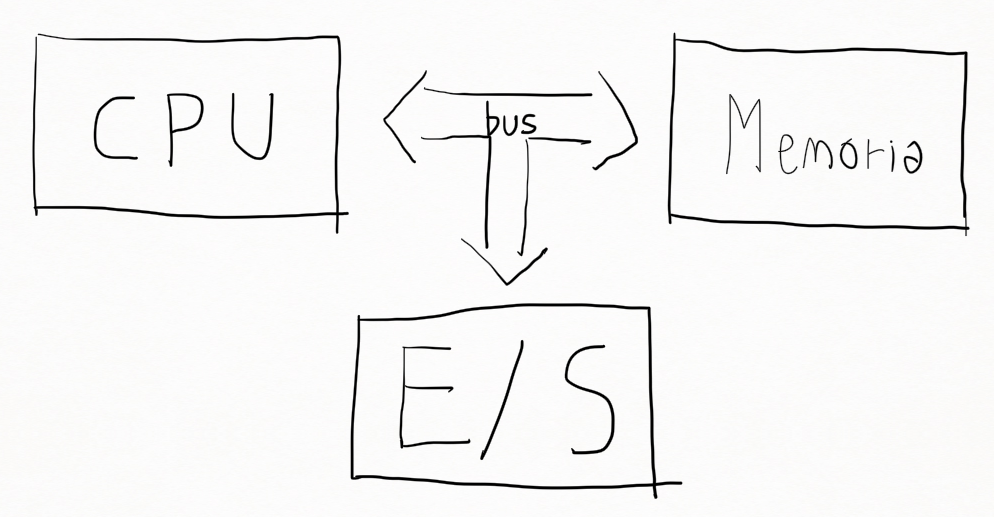
\includegraphics[scale=0.3]{ArqVN.png}
	\caption{Esquema de los componentes de la arquitectura de Von Neumann.}
	\label{fig-ArqVN}
\end{figure}

El procesador tiene tres componentes que cumplen distintas funciones: la unidad de control, la unidad aritmética lógica (ALU) y el banco de registros. La unidad aritmética lógica consta de varios circuitos combinatorios que implementan operaciones básicas, como por ejemplo operaciones lógicas como <<y>>, <<o>> y <<no>>, operaciones aritméticas como suma y multiplicación (para números codificado con una cantidad fija de bits) u operaciones básicas sobre cadenas e bits, como el {\sl shift}, que traslada cada bit un lugar a la derecha o la izquierda. El banco de registros consta de ciertos registros (un tipo de circuito que almacena valores) en general variables que se usan para el funcionamiento de la CPU. Por ejemplo, pueden tener los argumentos de las operaciones que va a realizar la unidad aritmética lógica. También hay un registro de particular importancia llamado {\sl program counter}, que indica la posición de memoria de la siguiente instrucción a ejecutar (es de suma importancia, ya que la idea del CPU es ejecutar secuencias de instrucciones). Finalmente, la unidad de control es un circuito secuencial que se encarga de llevar a cabo las instrucciones, usando la unidad aritmética lógica y el banco de registros. Estos circuitos secuenciales están hechos para que automáticamente se lea e identifique la instrucción que indica el program counter, se carguen nuevos datos en los registros (si es necesario), se realice la operación indicada en la ALU y se guarde el resultado donde corresponda (si hay que hacer alguna operación), y que el program counter avance a la siguiente instrucción, para poder repetir el proceso.

Respecto a la suma, la ALU al ser un circuito combinatorio, es en realidad como una tabla que tiene el resultado para cada combinación de operandos. Las sumas que se realizan directamente por la ALU pueden ser por ejemplo de números representados por uno o dos bytes (donde un byte es por definición una secuencia de 8 bits). Como la cantidad de números representables crece exponencialmente con la cantidad de bits, hacer sumas de números más grandes por la ALU (que lo que hace es tener una tabla con todos los resultados) es extremadamente ineficiente. Lo que se hace para realizar sumas con números más grandes es descomponerlas como una secuencia de instrucciones más sencillas. Esto es como lo que se hace en los algoritmos aritméticos básicos. Pensemos por ejemplo en el producto. Está la tabla de multiplicación que uno se aprende de memoria (lo cual es análogo a lo que está en los circuitos de la ALU) pero luego a partir de eso, siguiendo un algoritmo (secuencia de instrucciones) se puede calcular la multiplicación de números de cualquier cantidad de cifras sin precisar saber nada más de memoria.

La memoria es un dispositivo electrónico capaz de almacenar muchos valores, los cuales pueden ser leídos o modificados. Tiene la estructura de un gran vector de bytes, indizado por secuencias de bits de largo fijo. Por ejemplo, si se usan dos bits para indizar, los lugares de la memoria serían el {\tt 00}, el {\tt 01}, el {\tt 10} y el {\tt 11}, cada uno de los cuales contendría un byte de información. En las computadoras actuales la memoria suele tener del orden de $2^{32}$ lugares de memoria, es decir 4GB ($2^{10}$ bytes es un KB, $2^{20}$ es un MB y $2^{30}$ es un GB). Se trata de la llamada memoria RAM. Actualmente la cantidad de bits que se usa para indizar es 64 (la llamada arquitectura de 64 bits), pero eso no implica que todas las palabras que se puedan formar correspondan a direcciones válidas (en computadoras personales no existe actualmente memoria de $2^{64}$ bytes, que serían como 16 mil millones de gigabytes). Conceptualmente el banco de registros del procesador es como una memoria. El motivo de que existan las dos cosas es que el banco de registros es memoria de mejor calidad y más cara que se reserva para estar dentro de la CPU, mientras que la memoria RAM es más lenta pero más económica para tener en grandes cantidades.

\subsection{Ejemplo de programa}

Hagamos un ejemplo del funcionamiento de una computadora. Supongamos que tenemos 8 registros (enumerados) de un byte cada uno y que las direcciones de memoria son indizadas también por un byte. Supongamos que tenemos las siguientes instrucciones
\begin{itemize}
	\item {\tt LOAD}. Instrucción con dos parámetros: {\tt M} y {\tt R}, que lo que hace es cargar en el registro {\tt R} el contenido de la dirección de memoria {\tt M}.
	\item {\tt SAVE}. Instrucción con dos parámetros: {\tt M} y {\tt R}, que lo que hace es guardar en la dirección de memoria {\tt M} el contenido del registro {\tt R}.
	\item {\tt ADD}. Instrucción con tres parámetros: $\mathtt{R_1}$, $\mathtt{R_2}$ y $\mathtt{R_3}$ que lo que hace es sumar el contenido de los registros $\mathtt{R_1}$ y $\mathtt{R_2}$ y guardar el resultado en el registro $\mathtt{R_3}$.
\end{itemize}


Respecto a la operación {\tt ADD}, como los contenidos de los registros son bytes, o sea 8 bits, se considera que cada secuencia de 8 bits representa en binario un número entre $0$ y $2^8-1$. En caso de que el resultado se salga del rango, se le sustraye $2^8$ al resultado (formalmente, es la suma de $\mathbb{Z}_{2^8}$, es decir aritmética modular).

Por otra parte, cada instrucción está codificada por un byte. Supongamos que el código de {\tt LOAD} es {\tt 00000001}, el de {\tt SAVE} es {\tt 00000010} y el de {\tt ADD} es {\tt 00000011}.

Asumamos también que los tres primeros registros, $\mathtt{R_1}$, $\mathtt{R_2}$ y $\mathtt{R_3}$ se identifican con los bytes {\tt 00000001}, {\tt 00000010} y {\tt 00000011}.

Supongamos que queremos un programa que lo que haga es sumar los contenidos de las direcciones de memoria {\tt 10000001} y {\tt 10000010} y guardar el resultado en la dirercción {\tt 10000011}. Podríamos hacerlo realizando cuatro instrucciones. Primero un {\tt LOAD} para cargar el contenido de la primera dirección de memoria en el registro 1, luego otro {\tt LOAD} para cargar el contenido de la segunda dirección de memoria en el registro 2, luego un {\tt ADD} para sumar los contenidos de los registros 1 y 2 y guardar el resultado en el registro 3 y finalmente una {\tt SAVE} para guardar el contenido del registro 3 en la tercera dirección de memoria. Primero escribamos las instrucciones de un modo un poco más abstracto (para no ir de una a los 0s y 1s).  Definamos las direcciones de memoria {\tt 10000001}, {\tt 10000010} y {\tt 10000011} como $\mathtt{M_1}$, $\mathtt{M_2}$ y $\mathtt{M_3}$, respectivamente. El programa sería lo siguiente.
\begin{align*}
	&\mathtt{LOAD} \quad\mathtt{M_1~R_1}\\
	&\mathtt{LOAD}  \quad\mathtt{M_2~R_2}\\
	&\mathtt{ADD}  \quad\mathtt{R_1~R_2~R_3}\\
	&\mathtt{SAVE}  \quad\mathtt{M_3~R_3}
\end{align*} 
Esto último es lo que se considera como un programa escrito en {\sl assembler}. Es una forma de programar en la que cada línea es una instrucción del procesador, pero se pueden usar los nombres de las instrucciones y nombres de lugares de memoria, en lugar de tener que escribir todo en bits. El mismo programa escrito ahora en código máquina, es decir en bits, exactamente como iría en la memoria, sería:
\begin{align*}
	&\mathtt{00000001} \quad\mathtt{10000001~00000001}\\
	&\mathtt{00000001}  \quad\mathtt{10000010~00000010}\\
	&\mathtt{00000011}  \quad\mathtt{00000001~00000010~00000011}\\
	&\mathtt{00000010}  \quad\mathtt{10000011~00000011}
\end{align*}
La organización en líneas del código es para que sea más fácil de leer, pero el programa de hecho es simplemente 0000000110000001000000010000000110000010000000100000001100 0000010000001000000011000000101000001100000011. Si tenemos en alguna parte de la memoria esa secuencia de bytes y el program counter indicando la dirección donde comienza, la computadora automáticamente lo ejecutará. Esto se ilustra en la figura \ref{fig-ArqVNEjProg}.

Cabe resaltar que este es un ejemplo muy sencillo. Hay otros tipos de instrucciones (por ejemplo las que modifican el program counter y permiten realizar ciclos) y los programas suelen ser mucho más largos. De hecho, cuales son exactamente las instrucciones y cómo se codifican varía de un procesador a otro.

\begin{figure}
	\centering
	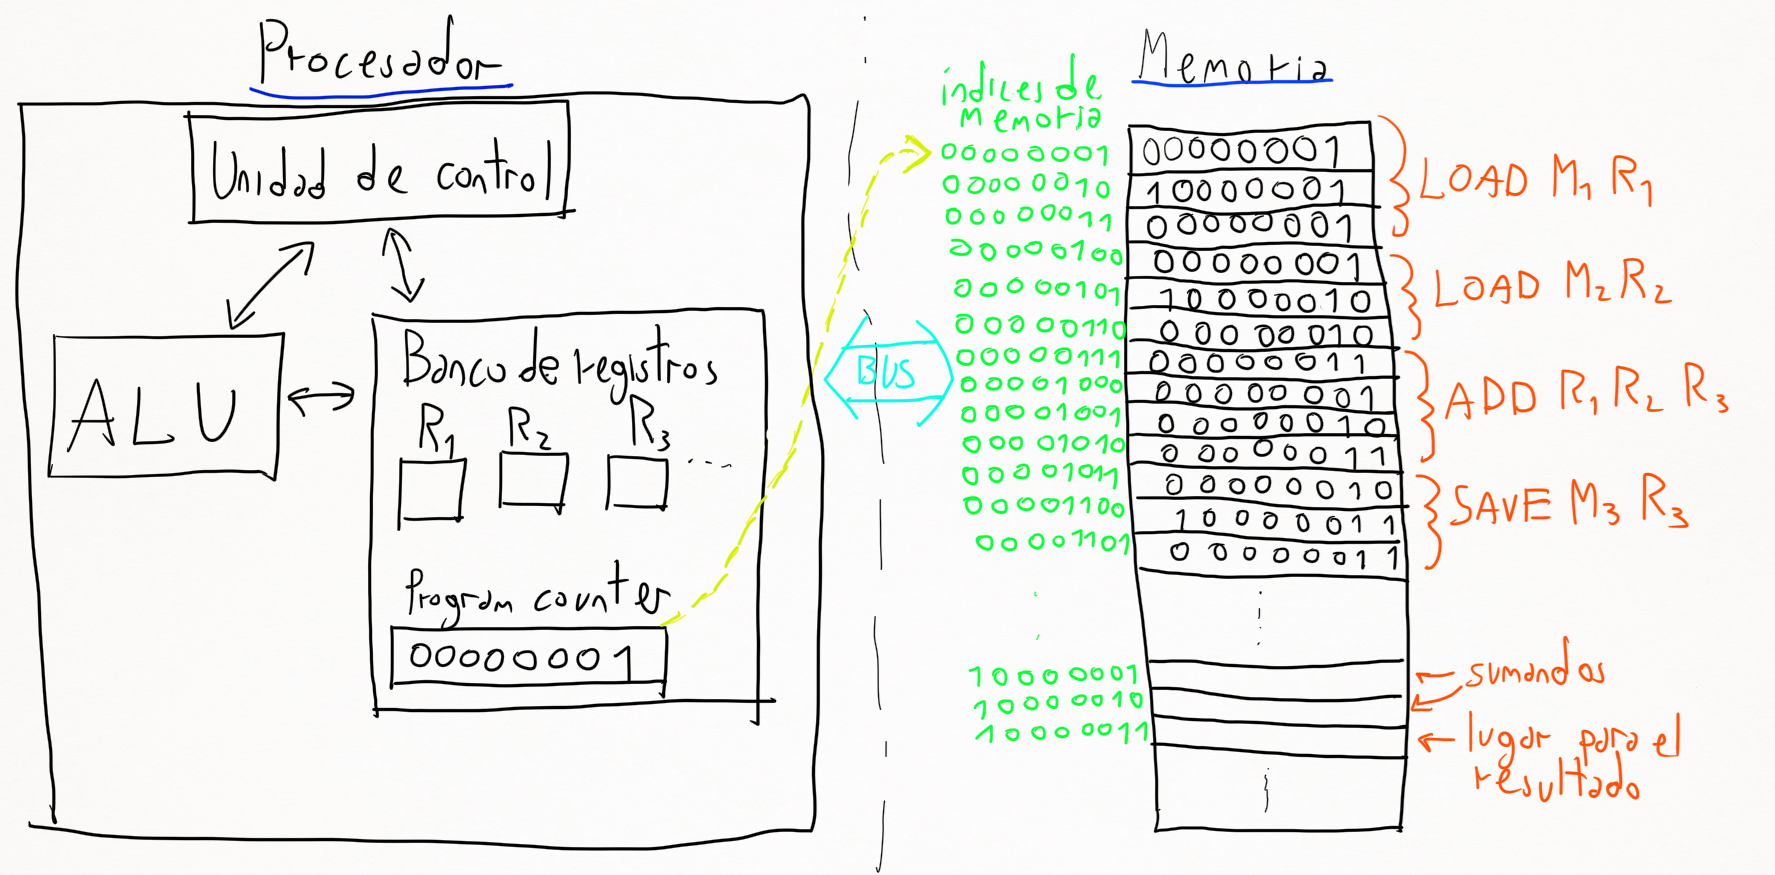
\includegraphics[scale=0.33]{ArqVNEjProg.png}
	\caption{Esquema de una computadora con un programa.}
	\label{fig-ArqVNEjProg}
\end{figure}

\section{Lenguajes de programación y compiladores}

Dada una computadora que sigue la arquitectura de Von Neumann, se puede implementar cualquier función computable con algún programa escrito en código máquina. Sin embargo, hay algunas características poco prácticas.
\begin{itemize}
	\item Es relativamente difícil escribir programas como secuencias de instrucciones de máquina. En general hay muchos más detalles que entran en juego que en el ejemplo dado y hace falta mucho esfuerzo para escribir programas que hagan operaciones complejas.
	\item Distintos procesadores suelen tener distintas instrucciones. Además, incluso cuando la instrucción es la misma puede estar codificada distinto. Por ejemplo, puede que en un procesador {\tt 00000001} sea el código de la suma y en otro sea el código de la operación de cargar en un registro. Por lo tanto, un programa que se escribe para un procesador probablemente no funcione en otro.
\end{itemize}
Estos factores dificultan escribir programas y hacen que solamente lo puedan hacer especialistas. Sin embargo, con el tiempo se desarrolló un concepto que mejora la situación, haciendo que sea más fácil desarrollar un programa y que la curva de aprendizaje sea más corta. Se trata de los {\bf lenguajes de programación}.

Los lenguajes de programación introducen abstracciones que permiten escribir programas sin preocuparse por detalles técnicos de cómo se resuelve con instrucciones del procesador. Por ejemplo, se introduce el concepto de las variables para trabajar con datos sin preocuparse por en qué direcciones de memoria están ni de cómo se utilizan los registros para operaciones. Por ejemplo, se si tenemos tres variables {\tt x, y} y {\tt z}, para sumar los contenidos de las primeras dos y guardarlo en la tarcera, simplemente habría que escribir:
$$\mathtt{z} = \mathtt{x}+\mathtt{y}
$$
sin preocuparse ni por en qué dirección va cada una ni de si hay que usar registros para realizar la suma o no.

Un programa escrito en un lenguaje de programación es un archivo de texto. Se compone por líneas escritas con caracteres comunes que representan operaciones de forma clara (para una persona). Las instrucciones escritas en un lenguaje de programación no pueden ser ejecutadas directamente por un procesador (estos solo entienden ceros y unos). En este punto entran en juego los {\bf compiladores}. Estos son programas cuya función es traducir un programa escrito en un lenguaje de programación a un programa en código máquina. Se los puede pensar como funciones cuya entrada es un programa escrito en un lenguaje de programación y su salida es una secuencia de instrucciones de procesador (lenguaje máquina) que hace lo mismo. El proceso usual al programar es el siguiente: primero se escribe el programa en un lenguaje de programación, luego se usa un compilador para traducirlo a código de máquina y finalmente se lo ejecuta.

Los lenguajes de programación junto con los compiladores solucionan las dos desventajas previamente mencionadas. Por una parte, escribir en un lenguaje de programación es más fácil que en lenguaje máquina. Por otra parte, un lenguaje de programación suele tener compiladores para distintos procesadores, de modo que un mismo programa escrito en este lenguaje puede ser compilado a código máquina de distintos procesadores y por lo tanto ser ejecutado en cada uno de ellos.

Se dice que un lenguaje de programación es de alto o bajo nivel según el nivel de abstracción que hay por sobre el lenguaje de máquina (instrucciones del procesador). Escribir directamente las instrucciones del procesador o código en assembler es de bajo nivel, mientras que usar un lenguaje de programación que incluye abstracciones como variables, estructuras de datos o iteraciones es de alto nivel. Entre los distintos lenguajes de programación hay varios niveles de abstracción.


El lenguaje {\tt c} (así como {\tt pascal}) es un lenguaje de relativamente bajo nivel, pues tiene abstracciones como las previamente mencionadas, pero no está {\sl tan} lejos del lenguaje máquina. Mirando un programa escrito en {\tt c}, para alguien con experiencia no es tan difícil darse cuenta de cómo podrían ser las instrucciones en lenguaje máquina.

Por otra parte, el lenguaje {\tt python}, que es el que usaremos en el curso, es de muy alto nivel. Esto significa que tiene abstracciones muy complejas por sobre el lenguaje máquina, las cuales hacen que se pueda programar en base a razonamientos intuitivos sin saber cómo se haría en lenguaje de máquina. De hecho puede ocurrir que una sola línea de código en {\tt python} corresponda a cientos de instrucciones del procesador, con lo que se resuelven automáticamente detalles técnicos y se le ahorra trabajo al programador. En general usar un lenguaje de programación de alto nivel es más fácil que usar uno de bajo nivel. La desventaja que tienen es que las abstracciones pueden hacer que el programa no sea lo más eficiente posible. En general un programa escrito en {\tt c} es mucho más rápido que uno equivalente en {\tt python} (pero mucho más difícil de escribir).


\chapter{Programación (en python)}\label{cap-prog}


En este capítulo se presentan los conceptos básicos para programar en el lenguaje python. Si bien se trata de un lenguaje específico, los conceptos se aplican de forma muy similar en otros.

Como material complementario, se recomienda el tutorial de la documentación oficial de python: \href{https://docs.python.org/es/3.13/tutorial/index.html}{https://docs.python.org/es/3.13/tutorial/index.html}. Ese tutorial contiene mucho más que lo que se necesita para el curso. Se recomienda ver todo el capítulo 3 y algunos conceptos del 4, pero sin preocuparse por detalles técnicos (hay explicaciones pensadas para gente que ya conoce conceptos de programación por otros lenguajes).

Cabe aclarar que lo que se ve en este curso es solo una pequeña introducción a python. Además, las explicaciones buscan transmitir ideas del lenguaje, sin necesariamente ser totalmente correcto con las definiciones formales de los conceptos o exactamente cómo funciona por dentro. Para esto se recomienda nuevamente la documentación (reiterando que excede los contenidos del curso).

\section{Instalación y ejecución}\label{sec-instalyEjec}

Instalar python es principalmente instalar el compilador que traduce el código en python a lenguaje máquina, de modo que podamos ejecutar lo que programemos. Un detalle técnico es que en lugar de llamársele <<compilador>> se le llama <<intérprete>>. Esto es porque en lugar de pasar todo el programa a lenguaje máquina y luego ejecutarlo, va pasando las líneas de código a lenguaje máquina una por una a la vez que se van ejecutando. Se dice que es un compilador cuando primero se traduce todo a lenguaje máquina y luego se lo ejecuta.

En el sistema operativo linux, en general python ya viene instalado por defecto. Por otra parte, en windows no es el caso (nos enfocaremos en este sistema operativo, ya que quienes utilizan linux es más probable que ya sepan ejecutar python). Una forma de instalarlo es descargando el instalador desde el sitio web de python y ejecutándolo (\href{https://www.python.org/downloads/}{https://www.python.org/downloads/}). Durante la instalación es importante marcar la opción de <<Add python.exe to PATH>> (figura \ref{fig-InstallPython}), por motivos que vermos a contiuación.

\begin{figure}
	\centering
	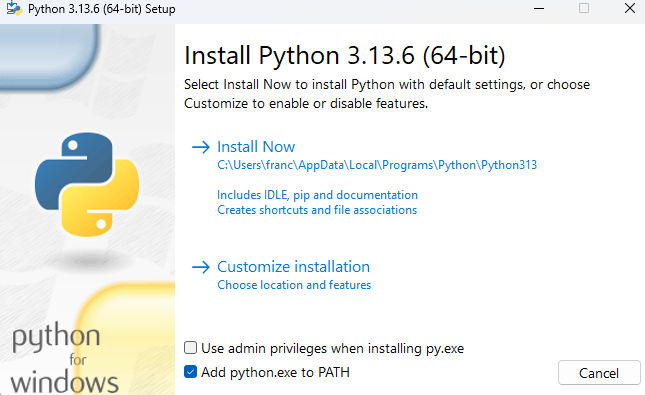
\includegraphics[scale=0.5]{InstallPython.png}
	\caption{Es importante marcar la opción <<Add python.exe to PATH>>.}
	\label{fig-InstallPython}
\end{figure}

Vamos a ejecutar python desde una ventana de comandos (o terminal). Esto es una ventana a través de la cual se le escriben comandos al sistema operativo. En windows se llama Windows PowerShell o símbolo del sistema.

Si hicimos bien la instalación de python, al abrir una ventana de comandos, si se escribe python y se toca enter, comienza a ejecutarse el intérprete, el cual nos permite ir ingresando instrucciones una a una. Los tres símbolos de >~significan que el intérprete está listo para recibir instrucciones. Una primera cosa que se puede hacer es usarlo como calculadora, escribiendo expresiones aritméticas y tocando enter (figura \ref{fig-cmdPython}). Para salir del intérprete se puede escribir {\tt quit()} y tocar enter.

Al escribir python, lo que se hace es ejecutar el intérprete. Para que esto funcione, el sistema operativo debe tener la dirección en la que python está instalado dentro de una cierta lista. Esto es lo que se hace al marcar la opción <<Add python.exe to PATH>> durante la instlación. Luego de haber ejecutado python en la ventana de comandos, el uso del intérprete ocurre dentro de esta misma ventana, sin usarse ninguna interfaz gráfica (a diferencia de la mayoría de los programas que utilizamos). En general no hay necesidad de nada más sofisticado.

\begin{figure}
	\centering
	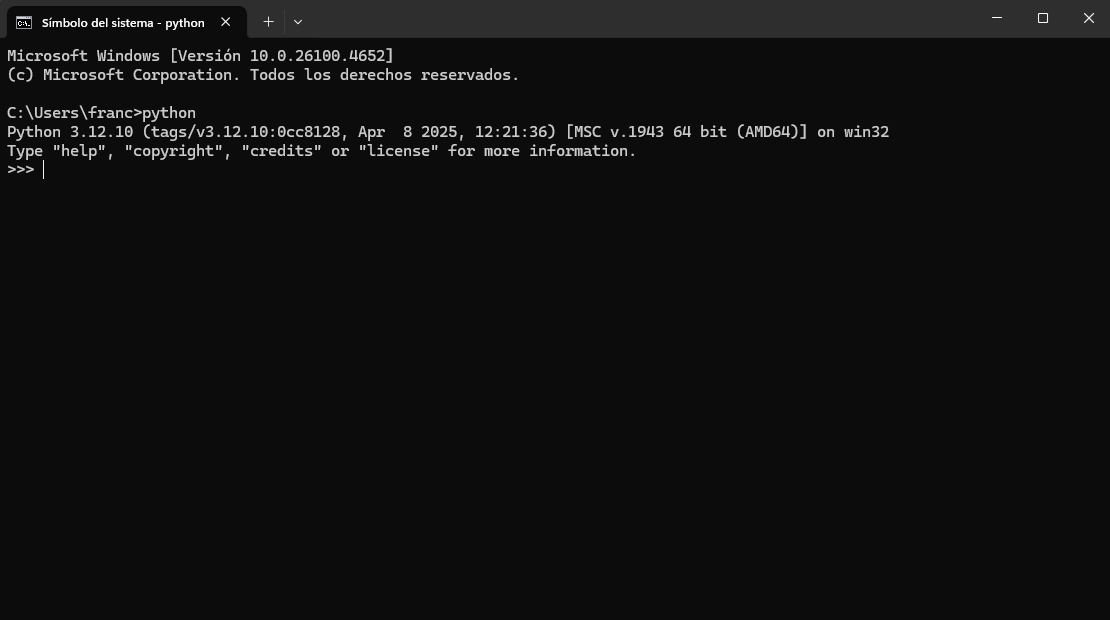
\includegraphics[scale=0.5]{cmdPython.png}
	\caption{Ventana de comandos con el intérprete de python.}
	\label{fig-cmdPython}
\end{figure}

Con la modalidad de uso del intérprete que vimos, se escriben y ejecutan lineas una a una. Por otra parte, se puede escribir un archivo con varias lineas de código y pasárselo al intérprete para que lo ejecute. El código se escribe en un archivo de formato <<.py>>. Para escribir este tipo de archivos se puede usar cualquier editor de texto, pero se recomienda utilizar un editor de código especializado. Uno muy popular actualmente es visual studio code (\href{https://code.visualstudio.com/}{https://code.visualstudio.com/}). Una vez que se escribió el archivo con el código y se lo tiene guardado en una carpeta, hay que abrir una ventana de comandos en esa carpeta (cada ventana de comandos trabaja en alguna carpeta particular) e ingresar <<python>> seguido del nombre del archivo con el <<.py>> incluido. Esto se ejemplifica en la figura \ref{fig-ejecPython}.

Para todo lo que mencionamos en esta sección, buscando en internet (motores de búsqueda como google, o sitios con contenido audiovisual como youtube) se encuentran muchos tutoriales. 

\begin{figure}
	\centering
	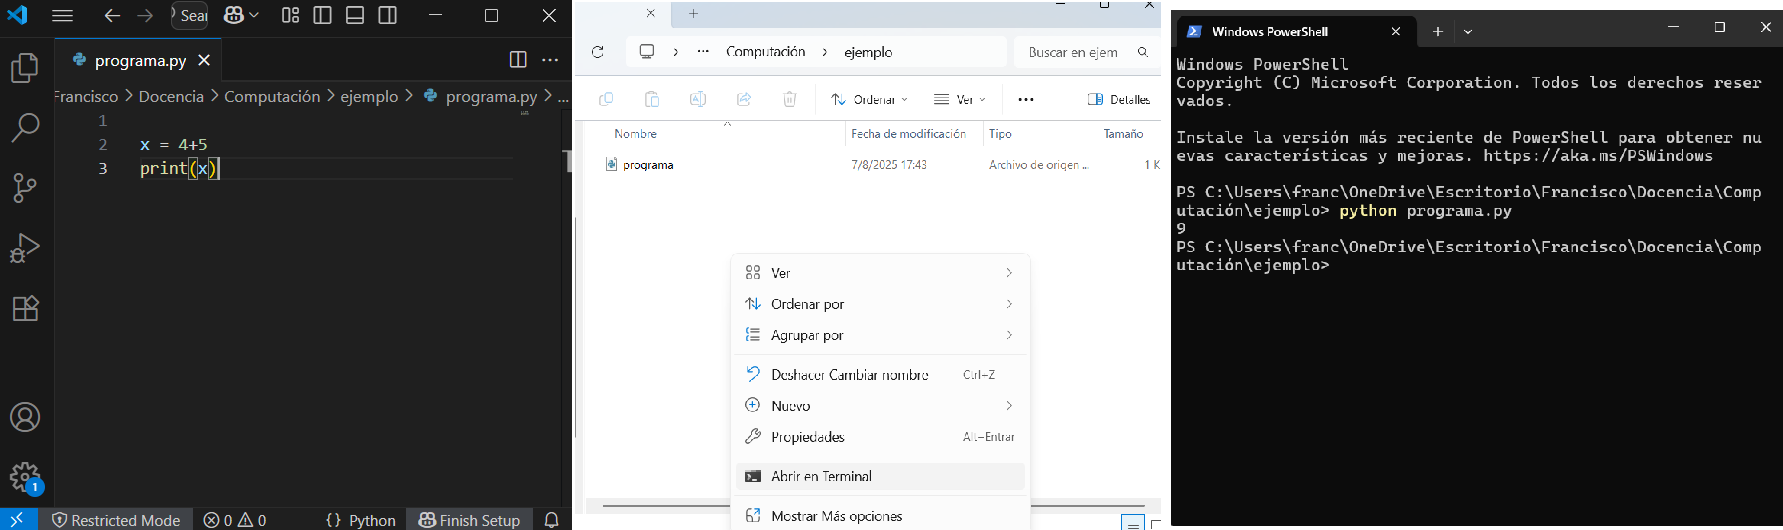
\includegraphics[scale=0.4]{ejecPython.png}
	\caption{A la izquierda visual studio code con el código del archivo llamado programa.py. Al centro se ve la carpeta llamada ejemplo en la que está el archivo. Dentro de esa carpeta se abre la terminal. A la derecha se ve la terminal en la que se escrie <<python programa.py>>. Antes del símbolo >, a la izquierda de <<python>>, se indica la carpeta en la que está la terminal. Si al hacer click derecho en la carpeta no aparece la opción <<abrir en terminal>>, puede aparecer al hacer click derecho manteniendo apretado mayus/shift (recordar que powershell también es una terminal). En todo caso, para problemas como este se recomienda buscar en internet, con lo cual se suele encontrar alguna solución rápidamente. También se puede abrir una terminal en cualquier sitio y cambiar la ubicación con instrucciones específicas, como {\tt cd} (buscar en internet en caso de que haya interés).}
	\label{fig-ejecPython}
\end{figure}
\section{Tipos de datos}

Una de las abstracciones que aportan los lenguajes de programación consiste en los tipos de datos. Se trata de la abstracción de distintos tipos de objetos, como enteros, texto o listas, cada uno de los cuales tiene distintos posibles valores y distintas operaciones que se pueden aplicar. Por supuesto que todos estos objetos se codifican como secuencias de bits, pero poder trabajar pensando en términos de objetos de distinto tipo hace que programar sea más intuitivo. Se puede saber el tipo de datos de un objeto escribiendo {\tt type()} con el objeto entre paréntesis. Veamos algunos de los tipos de datos que tiene python con algunas de las operaciones disponibles. 

\subsection{Booleanos}

Los booleanos conforman un tipo de datos que representa valores de verdad. Tiene solo dos objetos: {\tt True} y {\tt False}. Se tienen las operaciones lógicas básicas: {\tt not}, {\tt and} y {\tt or}. Hay algunos ejemplos en la figura \ref{fig-ejemploBool}. Si aplicamos {\tt type()} a un booleano, retorna {\tt class bool}. En general los booleanos por sí solos no suelen ser de mucha utilidad. Su principal aplicación es en condicionales e iteraciones, que estudiaremos en lo siguiente. 

\begin{figure}
	\centering
	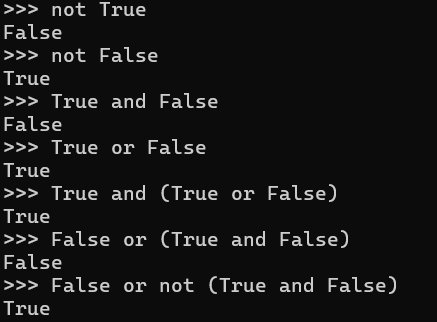
\includegraphics[scale=0.6]{ejemploBool.png}
	\caption{Ejemplos de operaciones con booleanos.}
	\label{fig-ejemploBool}
\end{figure}

\subsection{Enteros}

Se trata de un tipo de datos para representar enteros naturales. Los objetos son {\tt 0}, {\tt 1} {\tt -1}, {\tt 2}, {\tt -2}, etc. Si aplicamos {\tt type()} a un entero, retorna {\tt class int} por {\sl integer}. Tienen las operaciones aritméticas elementales, que se muestran en la figura \ref{fig-ejemploInt}. Notar que la división entera es con dos barras. Una barra sola es otra operación que veremos en la brevedad. Por otra parte se tienen las operaciones de comparación, que reciben dos enteros y retornan un booleano. Se muestran en la figura \ref{fig-ejemploComp}. En el caso de la igualdad, si se escribe un solo símbolo <<=>> es una asignación, lo cual veremos más adelante.

\begin{figure}
	\centering
	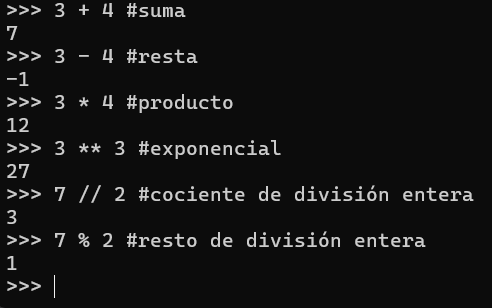
\includegraphics[scale=0.6]{ejemploInt.png}
	\caption{Operaciones aritméticas básicas. Lo que está escrito después de los \# son comentarios. Los comentarios son ignorados por el intérprete, la función que cumplen es de aclaraciones para personas que lo leen.}
	\label{fig-ejemploInt}
\end{figure}

\begin{figure}
	\centering
	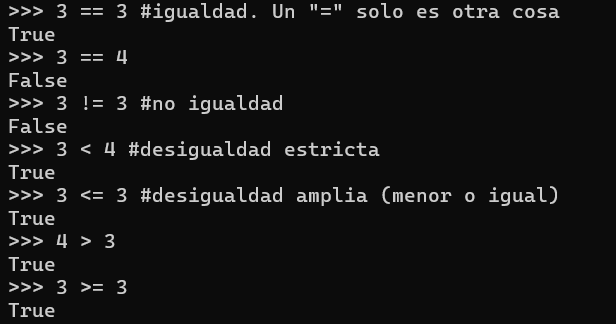
\includegraphics[scale=0.6]{ejemploComp.png}
	\caption{Comparaciones entre enteros. }
	\label{fig-ejemploComp}
\end{figure}

\subsection{Números de punto flotante} \label{sec-float}

Se trata de una representación para operar con números reales usando información finita. De hecho lo que representan es un conjunto finito de números racionales, pero a menos de cierta aproximación se opera con ellos igual que con números reales. Estos números se escriben con la notación usual para números con parte fraccionaria o con notación científica, en ambos casos separando la parte fraccionaria con un punto. Están las mismas operaciones aritméticas y comparaciones, salvo por la división. En punto flotante tenemos el operador / para la división de números reales. Un detalle importante es que si aplicamos la operación / a enteros, el resultado es de punto flotante, independientemente de que la división de exacta o no. Se presentan ejemplos en la figura \ref{fig-ejemploFloat}.

Los números de punto flotante tienen limitaciones debido al hecho de que se pueden representar solo finitos números. Por ejemplo, si a {\tt 1.0} le sumamos un número muy chico, se redondea a {\tt 1.0}, lo cual puede ser problemático en algunas situaciones. Ignoraremos este problema, pero es un tema relevante dentro del área de análisis numérico.

Hay más operaciones sobre punto flotante que se pueden realizar si importamos la biblioteca {\tt math}. Más adelante en el curso nos centraremos más en las bibliotecas, pero por ahora alcanza con saber que es algo que permite extender el lenguaje con más operaciones. Para incluir el contenido de la biblioteca {\tt math} hay que escribir la instrucción {\tt import math}. Después de eso se pueden utilizar las operaciones incluidas en esta biblioteca. Esto se hace escribiendo el nombre de la biblioteca, un punto y el nombre de la operación. Por ejemplo, tiene una operación de raiz cuadrada que se utiliza escribiendo {\tt math.sqrt()}, donde al argumento lo ponemos entre los paréntesis. Por otra parte, está la operación {\tt math.floor()} que retorna el entero más cercano a la izquierda. Esta última función retorna efectivamente un objeto de tipo entero y no un objeto de tipo punto flotante con valor entero. Se presentan ejemplos en la figura \ref{fig-ejemploMath}.

En general se pueden realizar operaciones aritméticas entre enteros y números de punto flotante. En ese caso, el resultado es de punto flotante. Lo que ocurre en estos casos es que (al menos conceptualmente) se convierten automáticamente enteros a punto flotante. Al aplicar / a enteros ocurre lo mismo (al menos conceptualmente): primero los enteros se transforman a punto flotante y luego se aplica la operación. Por otra parte, en general no hay conversión automática de punto flotante a entero, aunque el número no tenga parte fraccionaria.

\begin{figure}
	\centering
	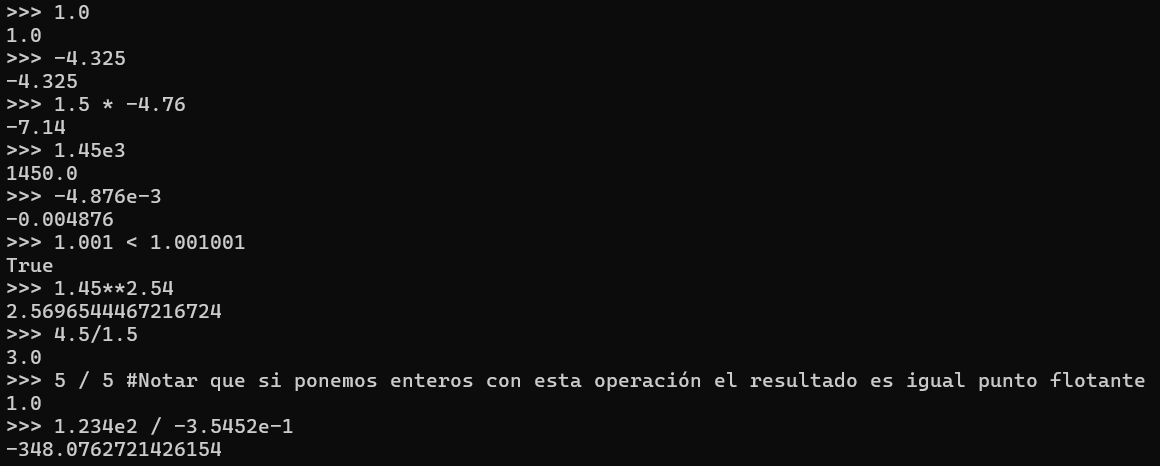
\includegraphics[scale=0.6]{ejemploFloat.png}
	\caption{Ejemplos de números de punto flotante.}
	\label{fig-ejemploFloat}
\end{figure}

\begin{figure}
	\centering
	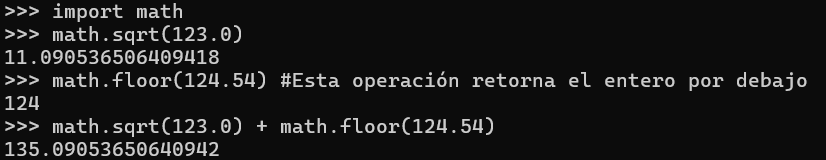
\includegraphics[scale=0.6]{ejemploMath.png}
	\caption{Ejemplos de operaciones de la biblioteca math.}
	\label{fig-ejemploMath}
\end{figure}


\subsection{Texto}

En python se puede representar texto como secuencias de caracteres, denominadas {\sl strings}. Los strings se delimitan con comillas simples o dobles. Si aplicamos {\tt type()} a un string, retorna {\tt class str}. Los caracteres pueden ser por ejemplo letras, dígitos, signos de puntuación, espacios o caracteres especiales para representar cosas como el salto de línea (pasar a la siguiente línea). Algunos ejemplos de strings son ``Hola.'', ``345'', `` '' (espacio)  y ``\hspace{0.1em}'' (string vacío). No hay que confundir, por ejemplo, al string ``345'' con el entero {\tt 345}, pues son objetos de distintos tipos (se lo puede verificar con {\tt type()}). Con el símbolo + se realiza la operación de concatenación, es decir ``Hola.'' + ``345'' da ``Hola.325''. Notar que el símbolo + tiene varios usos. Cual de todos se usa depende del tipo de los argumentos. Por ejemplo, {\tt 12 + 12} da {\tt 24} (los argumentos son enteros, por lo que se los suma), mientras que {\tt ``12'' + ``12''} da {\tt ``1212''} (los argumentos son strings, por lo que se los concatena). Si se ejecuta {\tt 12 + ``12''} da un error por los tipos.

Por otra parte, se pueden realizar con strings las mismas comparaciones que con números. La igualdad {\tt ==} y la desigualdad {\tt !=} determinan si se trata de exactamente el mismo string o no, mientras que las desigualdades usan orden lexicográfico.

\subsection{Listas}

Las listas conforman un tipo de datos compuesto. Cada lista es, como su nombre sugiere, una lista de objetos. Una lista se comienza y se termina con <<[>> y <<]>>. Los distintos elementos se separan con comas. Por ejemplo: {\tt[0,1,4]}, {\tt[``aa'',``a'',``'']}, {\tt [3.5, ``a'']} y {\tt[]}. Las listas pueden tener cualquier cantidad de elementos (a partir de cero) y estos elementos pueden ser de cualquier tipo, incluso otras listas. Por ejemplo {\tt [[],[]]} es una lista con dos elementos, que los dos son la lista vacía. Con + se puede concatenar listas, de modo que {\tt [[],[]] + [1]} da {\tt [[],[],1]}.

Hay una operación de pertenencia, para la que se usa la palabra {\tt in}. La forma de aplicarlo es {\tt <<$x$ in $l$>>}, siendo $x$ un objeto y $l$ una lista. Esta operación retorna un booleano, el cual es {\tt True} si $x$ está en la lista $l$ y {\tt False} en otro caso. Por ejemplo, {\tt 3 in [1,2,3]} da {\tt True} mientras que {\tt 4 in [1,2,3]} da {\tt Fasle}. Para esta operación se piensa a la lista como un conjunto, en el sentido de que el resultado no se ve afectado por el orden de los elementos ni por si aparecen repetidos o no. A modo de ejemplo, {\tt 3 in [1,2,3]} da lo mismo que {\tt 3 in [3,2,1]} y que {\tt 3 in [3,3,2,1,1,3]}.

\subsection{Transformación entre tipos}\label{sec-TransfTipos}

En python hay ciertas operaciones que convierten un objeto a cierto tipo. Por ejemplo tenemos {\tt int()}, {\tt float()} y {\tt str()}, que permiten cambiar un objeto a entero, punto flotante o string, respectivamente.

La operación {\tt int()} se puede aplicar a un número en punto flotante o a un string. En caso de aplicarse a un número en punto flotante, se lo trunca. En caso de aplicarse a un string, si este string representa un entero retorna el entero y en otro caso da un error.

La operación {\tt float()} se puede aplicar a un número entero o a un string. En caso de aplicarse a un string, si este string representa un número en punto flotante, retorna este número y en otro caso da un error.

La operación {\tt str()} convierte el objeto en cuestión a un string y en general se puede aplicar a cualquier tipo. Los siguientes son algunos ejemplos.
\begin{verbatim}
>>> int(1.0)
1
>>> int(1.1)
1
>>> int(0.9)
0
>>> int("34")
34
>>> int("-34")
-34
>>> int("-34d") #da error
Traceback (most recent call last):
File "<stdin>", line 1, in <module>
ValueError: invalid literal for int() with base 10: '-34d'
>>> float(4)
4.0
>>> float("-4.634")
-4.634
>>> str(6)
'6'
>>> str(6.845)
'6.845'
\end{verbatim}

\section{Variables, expresiones y asignaciones}

Las {\bf variables} son objetos sintácticos (es decir elementos del lenguaje) que consisten en un nombre, el cual se puede usar para referenciar distintos objetos de cualquier tipo de datos. Diremos que el objeto referenciado es el valor de la variable. Es una abstracción para usar la memoria de modo intuitivo, en base a un nombre. Durante la ejecución de un programa, el objeto referenciado por una variable puede ir variando. Nombres válidos de variable son secuencias de caracteres alfanuméricos y <<\_>> en los que el primer carácter no es un número, como por ejemplo {\tt x, x1, total} y {\tt altura\_caja}. Hay ciertas palabras reservadas para usos especiales, las cuales no pueden ser usadas como variables, como por ejemplo {\tt if, for} y {\tt while}, cuyos usos veremos más adelante en este capítulo.

Las {\bf expresiones} son objetos sintácticos que se pueden calcular, resultando en un objeto de algún tipo de datos (que puede ser cualquiera). Están definidas en base a los siguientes casos.
\begin{enumerate}
	\item Los valores constantes (llamados {\sl lieterales} en python) de cualquier tipo son expresiones válidas. Por ejemplo, {\tt False}, {\tt 10}, {\tt ``Hola''} y {\tt[1,2,3]}. Estas expresiones al calcularse retornan el valor constante en cuestión.
	\item Una variable es una expresión válida. Al calcularse retorna el valor actual de la variable.
	\item Dada una operación, al aplicarla a ciertas expresiones, da lugar a una nueva expresión más compleja. Por ejemplo, <<{\tt 3+7}>>, <<{\tt 3**(5-2)}>>, <<{\tt x + 10}>>, <<{\tt x*y + z/2}>> y <<{\tt flag and (x<y)}>>. Como en varios de estos ejemplos, se puede aplicar una operación a expresiones que ya tienen operaciones. Al calcular la expresión, se realiza la operación correspondiente. Si {\tt x,y,z} tiene los valores $1,2,3$ respectivamente y {\tt flag} tiene le valor {\tt True}, entonces la expresiones calculan {\tt 10}, {\tt 27}, {\tt 11}, {\tt 3.5} y {\tt True}, respectivamente.
	
	Formalmente, dada una expresión definida por una operación entre otras dos expresiones {\tt exp1 op exp2}, para calcularla primero se calculan {\tt exp1} y {\tt exp2} en objetos $x_1$ y $x_2$ y luego se realiza la operación {\tt op} entre $x_1$ y $x_2$.
	
	\item Una función (elemento que se presenta la sección \ref{sec-funciones}) aplicada a ciertos argumentos (que pueden ser otras expresiones) da lugar a una expresión más compleja. Para calcular la expresión se evalúa la función. Por ejemplo, si tenemos definida una función {\tt f} con dos parámetros, entonces  {\tt f(4,9)}, {\tt f(x,2*(x+y))} y {\tt f(f(x,2),f(1,y))} son ejemplos de expresiones válidas.
	
	Forlamente, dada una expresión del tipo {\tt f(exp1, exp2,\dots,exp$n$)}, para calcularla primero se calculan las $n$ expresiones de los argumentos, dando $n$ objetos, luego se evalúa {\tt f} con estos objetos y lo que retorna {\tt f} es el resultado.
\end{enumerate}

La {\bf asignación} es la instrucción básica de python para dar un valor a una variable. La sintaxis es:
$$\mathtt{var}~=~\mathtt{expr}$$
donde $\mathtt{var}$ es el nombre de la variable a la que queremos asignar un objeto (es decir, hacer que la variable referencia al objeto, o que el objeto sea el valor de la variable) y $\mathtt{expr}$ es una expresión que calcula el objeto a asignar. Es distinto al uso que se le da al símbolo <<$=$>> en matemáticas (en particular, los lados tienen roles distintos), asemejándose más al de <<$:=$>>.



Al ejecutarse una asignación se hacen las siguientes dos cosas.
\begin{enumerate}
	\item Se calcula la expresión de la derecha.
	\item Se asocia ese objeto a la variable de la izquierda
\end{enumerate}
Si en la expresión hay alguna variable que no se ha definido antes o una operación aplicada a objetos de tipo incorrecto (por ejemplo {\tt ``a'' / [1,2] }), se produce un error.

La expresión puede contener la misma variable {\tt var}. En ese caso para evaluarla se usa el valor actual de la variable y luego se le asigna el resultado.

Los siguientes son algunos ejemplos. Lo que se escribe después del \# es un {\bf comentario}: está solo para aclarar algo a la persona que lee; python lo ignora.

\begin{verbatim}
>>> x = 10 #asignamos el valor 10 a la variable x
>>> x #Mostrar el valor actual de la variable x
10
>>> x*2
20
>>> x1 = x**2
>>> x1
100
>>> x = x + 1
>>> x
11
>>> z = 20
>>> z = z + x2 #Usamos una variable x2 que no definimos antes. Da error
Traceback (most recent call last):
File "<stdin>", line 1, in <module>
NameError: name 'x2' is not defined. Did you mean: 'x'?
>>> flag = True
>>> y = flag and x < 20
>>> y
True
>>> lista1 = ["a","b","c"]
>>> lista2 = [1,2,3]
>>> lista3 = lista1 + lista2
>>> lista3
['a', 'b', 'c', 1, 2, 3]
\end{verbatim}
En python las variables no guardan un valor dentro de ellas, sino que en realidad referencian a un objeto que está fuera en otro lado. Esto es un detalle técnico al que volveremos en la sección \ref{sec-memoriaCompartida}.
\section{Indizado y slicing}

En listas y en strings cada lugar tiene un índice, que es un entero no negativo. El primer lugar es el de índice {\tt 0}, el segundo es el de índice {\tt 1} y así sucesivamente. Notar que {\bf el primer luegar tiene índice 0}. Por ejemplo dada la lista {\tt [5,6,7]}, elemento de índice {\tt 0} es {\tt 5}, el de índice {\tt 1} es {\tt 6} y el de índice {\tt 2} es {\tt 7}. No hay elementos de índices mayores a {\tt 2}. Análogamente, dado un string {\tt``Hola''}, el elemento de índice {\tt 0} es {\tt ``H''}, el de índice {\tt 1} es {\tt ``o''}, el de índice {\tt 2} es {\tt``l''} y el de índice {\tt 3} es {\tt ``a''}. No hay elementos de índice mayor a {\tt 3}.

El {\bf indizado} es una operación para acceder al elemento de un índice dado en una lista o un string. La forma de escribirlo es {\tt x[n]}, donde {\tt x} es la lista o string y {\tt n} es el índice. Por ejemplo, si {\tt x} es {\tt [5,6,7]}, entonces {\tt x[0]} da {\tt 5}, {\tt x[1]} da {\tt 6} y {\tt x[2]} da {\tt 7}, mientras que si {\tt y} es {\tt``Hola''}, entonces {\tt y[0]} da {\tt ``H''}, {\tt y[1]} da {\tt ``o''}, {\tt y[2]} da {\tt ``l''}, y {\tt y[3]} da {\tt ``a''}.

Si tenemos una lista de números y le aplicamos indizado, el objeto resultante es un número. Por otra parte, cuando aplicamos indizado a un string, el objeto resultante no es de otro tipo, sino que también es un string, solo que de largo 1, ya que contiene solo el caracter del índice dado.



Tanto para listas como para strings, si el índice se pasa del último elemento, se produce un error. En python se puede usar la función {\tt len()} para determinar el largo de una lista o un string. Por ejemplo, {\tt len([5,6,7])} da 3 y {\tt len(``Hola'')} da 4. Los índices válidos de una lista o string {\tt x}, van desde {\tt 0} hasta {\tt len(x)-1}.

Por otra parte, el {\bf slicing} es una operación para obtener una sublista o un substring a partir de un rango de índices. En python los rangos se escriben con el símbolo <<:>> y se toma la convención de que son con {\bf orden inclusivo a la izquierda y estricto a la derecha}. Es decir, dados dos enteros no negativos $n<m$, tenemos que $n:m$ representa el intervalo cerrado a izquierda y abierto a derecha $[n,m)$. Dada una lista o string {\tt x} y dos enteros no negativos $n<m$, la operación de slicing se escribe {\tt x[$n:m$]} y resulta en la sublista o substring con los objetos de los índices pertenecientes al rango dado. Equivalentemente, da la sublista o substring de todos los elementos con índice $i$ tal que $n\leq i < m$. No hay problemas si nos pasamos del último elemento. El resultado puede ser la lista vacía o el string vacío.

El resultado de el slicing es una lista nueva, cuyos índices están dados por los lugares como con cualquier otra lista, sin tener por qué ser los mismos que en la lista anterior. Por ejemplo, si {\tt x} es la lista {\tt [5,6,7]}, el slicing {\tt x[1:3]} retorna la lista con los elementos de índices {\tt 1} y {\tt 2}, que es {\tt [6,7]}, pero los índices de esta nueva lista son {\tt 0}, para el primer lugar y {\tt 1} para el segundo. El {\tt 6} pasó a tener índice {\tt 0} y el {\tt 7} a tener índice {\tt 1}. Hay que recordar que los índices se definen por los lugares y no por los objetos que hayan. 

En una lista se pueden hacer asignaciones a elementos de cierto índice, modificando el objeto de ese lugar. Por ejemplo, si {\tt x} es la lista {\tt [5,6,7]}, la asignación {\tt x[1]=3} hace que pase a ser {\tt [5,3,7]}. Con strings no se permite hacer esto.

Hasta ahora venimos escribiendo {\tt x[n]} o {\tt x[n:m]}, donde {\tt x} es una variable y {\tt n} y {\tt m} son números específicos, pero cabe aclarar que en el lugar de {\tt n} y {\tt m} se pueden poner variables con valores numéricos, o en general cualquier expresión que calcule un número. De hecho, en el lugar de {\tt x} se puede también poner cualquier expresión que calcule una lista o un string. Por otra parte, como el indizado y el slicing son operaciones, pueden formar parte de expresiones, como por ejemplo {\tt x[n+1] - m}.

Veamos algunos ejemplos.
\begin{verbatim}
>>> x = [1,2,3,4,5]
>>> s = "Hola 1."
>>> x[0]
1
>>> s[1]
'o'
>>> s[4] #Va a retornar un espacio
' '
>>> len(s)
7
>>> s[6]
'.'
>>> s[7]
Traceback (most recent call last):
File "<stdin>", line 1, in <module>
IndexError: string index out of range
>>> x[5]
Traceback (most recent call last):
File "<stdin>", line 1, in <module>
IndexError: list index out of range
>>> x[0:2]
[1, 2]
>>> x[2:5]
[3, 4, 5]
>>> x[2:10]
[3, 4, 5]
>>> x[6:10]
[]
>>> x[1]=40
>>> x
[1, 40, 3, 4, 5]
>>> x[3*5-11]
5
>>> n = 3
>>> x[n]
4
>>> x[n-1] + 2
5
\end{verbatim}

Con listas de listas se puede concatenar indizados. Es decir, si {\tt l} es una lista cuyos elementos son listas, {\tt l[i][j]} es el {\tt j}ésimo elemento de la {\tt i}ésima lista. Los paréntesis implícitos van de la siguiente forma: {\tt (l[i])[j]}, pues {\tt l[i]} es una lista a la cual se aplica el índice {\tt j}. A modo de ejemplo:
\begin{verbatim}
>>> l = [[1,2],[3,4],[5,6]]
>>> len(l) #Tiene 3 elementos que son las listas de adentro
3
>>> l[0] # Retorna la primera lista
[1, 2]
>>> l[1] # Retorna la segunda lista
[3, 4]
>>> l[2] # Retorna la tercera lista
[5, 6]
>>> l[3] # Produzcamos un error de índice
Traceback (most recent call last):
File "<stdin>", line 1, in <module>
IndexError: list index out of range
>>> len(l[0]) #Largo de la lista [1,2]
2
>>> l[0][0] #Elemento 0 de lista 0
1
>>> l[0][1] #Elemento 1 de lista 0
2
>>> l[1][0] #Elemento 0 de lista 1
3
\end{verbatim}
En general de hecho, en caso de que {\tt l[i]} sea una lista, se puede hacer con ella lo mismo que con una lista que esté dada por una variable. Por ejemplo, también se puede hacer slicing con {\tt l[i][n:m]}, lo cual dará la sublista de {\tt l[i]} correspondiente, o determinar su largo con {\tt len(l[i])}. Por otra parte, también se puede asignar {\tt l[i]} a una variable nueva y luego trabajar con ella. Por ejemplo, hacer {\tt y = l[i]} y luego {\tt y[j]}, {\tt y[n:m]} o {\tt len(y)}, dando iguales resultados que {\tt l[i][j]}, {\tt l[i][n:m]} y {\tt len(l[i])}, respectivamente.
\subsection{Referencias múltiples}\label{sec-memoriaCompartida}

Vamos a tratar un detalle un poco técnico. La mayoría de las veces no es relevante, pero a veces puede ser fuente de errores inesperados.

Recordar que las variables no contienen los objetos, sino que los referencian. Esto es particularmente importante con listas porque estas se pueden modificar, entonces si dos variables referencian la misma lista y desde una la modificamos, esto se reflejará en la otra variable. Veamos un ejemplo.
\begin{verbatim}
>>> l1 = [1,2,3]
>>> l2 = l1
>>> l2[0] = 0
>>> l1
[0, 2, 3]
\end{verbatim}
Esto ocurrió porque la asignación {\tt l2=l1} lo que hizo es que la variable {\tt l2} referencie la misma lista que {\tt l1}. Para que la lista de {\tt l2} sea una lista distinta a la de {\tt l1} pero con los mismos valores, habría que escribir {\tt l2 = l1.copy()}.

Con números una asignación de una variable a otra también hace que referencie al mismo objeto, pero no surgen problemas. Por ejemplo:
\begin{verbatim}
>>> x=3
>>> y = x
>>> y = 0
>>> x
3
\end{verbatim}
La primera instrucción liga la variable {\tt x} al objeto {\tt 3}. La segunda instrucción liga la variable {\tt y} al mismo objeto. Sin embargo, la tercara instrucción lo que hace es ligar la variable {\tt y} a un nuevo objeto {\tt 0}, sin alterar el objeto {\tt 3} preexistente.

De hecho los dos ejemplos que presentamos son muy distintos. La asignación {\tt y=0} modifica a qué está asignada la variable {\tt y}; se podría decir que modifica la variable. Por otra parte, la operación {\tt l2[0]=0} modifica la lista referenciado por la variable {\tt l2}, sin cambiar el hecho de que esta variable está ligada a esa lista; se podría decir que modifica al objeto ligado a la variable y no a la variable. Ver la figura \ref{fig-ejemploVarMem}.

\begin{figure}
	\centering
	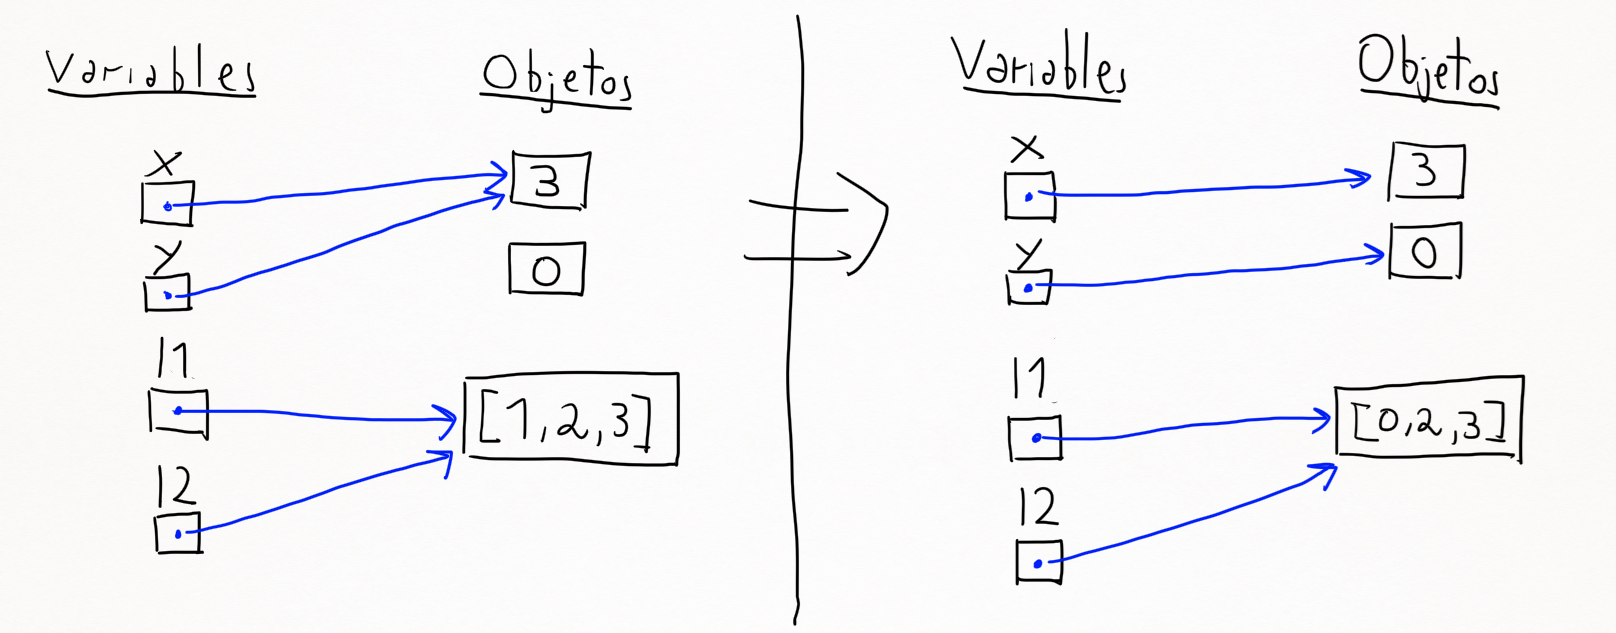
\includegraphics[scale=0.3]{ejemploVarMem.png}
	\caption{Ilustración de ejemplo presentado en la sección \ref{sec-memoriaCompartida}}
	\label{fig-ejemploVarMem}
\end{figure}

Los números son objetos {\bf inmutables}: no se pueden modificar. Las listas, por otra parte, son objetos {\bf mutables}, lo cual significa que pueden ser modificadas. Un ejemplo es cuando se modifica uno de sus elementos, como al ejecutar {\tt l2[0]=0}. Esta distinción de mutable o inmutable se aplica a los objetos de python en general. Los strings por ejemplo también son inmutables.



\section{Programas e instrucciones}

Digamos que programa en python es una secuencia de instrucciones que se almacena en un archivo de formato <<{\tt .py}>>. Un ejemplo básico de instrucción es la asignación, que ya vimos. Por otra parte, cuando escribimos una expresión o una variable en el intérprete y damos enter para que imprima el valor, también se trata de una instrucción. Estas últimas en general se usan solamente haciendo experimentos sencillos en el intérprete; no es común incluirlas en programas.

Al ejecutar un programa (ver figura \ref{fig-ejecPython}) se ejecutan las instrucciones en el orden que están escritas, es decir, de la primera línea en adelante, o desde arriba hacia abajo. No obstante, veremos que hay instrucciones de tipo condicional y de iteraciones, que adentro permiten hacer bifurcaciones (en base a alguna condición, lo que se ejecuta puede cambiar) o ciclos en la ejecución, respectivamente.

Digamos que las instrucciones pueden ser simples o compuestas. No es una distinción general, pero la introduzco porque me parece pedagógicamente útil en este punto. Las instrucciones simples son las que se escriben en una línea y representan una acción específica, mientras que las compuestas son instrucciones con cierta estructura que contienen adentro otras instrucciones. Las asignaciones son instrucciones simples y en esta sección presentamos algunas otras. En secciones posteriores presentaremos algunas instrucciones compuestas que son los condicionales y las iteraciones: {\tt if}, {\tt for} y {\tt while}.

Además de asignaciones, utilizaremos las siguientes instrucciones simples.
\begin{itemize}
	\item {\tt print()}. Se trata de una instrucción que imprime en la consola lo que se le pasa como parámetro. Es la instrucción por excelencia para mostrar algo en la consola. Si se le pasa un valor directamente imprime ese valor, mientras que si se le pasa una variable imprime el contenido de la variable. Por ejemplo, la instrucción {\tt print("Hola")} imprime <<Hola>>, mientras que {\tt print(x)} imprime el valor de la variable {\tt x} (y si esta variable no tiene ningún valor, da error).
	
	\item {\tt append()}. Esta instrucción es para agregar un elemento al final de una lista. A diferencia de las anteriores, es formalmente lo que se llama un {\sl método} de las listas. Dada una lista {\tt l} y un objeto $x$ que queremos agregar al final, la instrucción es {\tt l.append($x$)}. Se escribe el nombre de la lista, un punto y luego {\tt append()} con lo que queramos agregar adentro de los paréntesis.
	
	\item {\tt insert()} Permite agregar un elemento en un lugar particular de una lista. Al igual que {\tt append}, es un método. Dada una lista {\tt l}, un índice {\tt i} y un objeto $x$, la instrucción {\tt l.insert(i,$x$)} agrega al objeto $x$ en la posición de índice {\tt i} de la lista, moviendo a todos los elementos posteriores (en caso de que los haya) un índice adelante (por ejemplo, el {\tt i}-ésimo pasa a ser el nuevo {\tt(i+1)}-ésimo). A modo de ejempo, si {\tt l = [5,6,7]}, entonces si hacemos {\tt l.insert(1,0)} pasa a ser {\tt l = [5,0,6,7]}.
	
	\item {\tt del}. Permite (entre otras cosas) quitar el elemento de cierto índice de una lista. Dada una lista {\tt l}, la instrucción {\tt del l[i]} quita el elemento de índice {\tt i}. Si hay elementos después del {\tt i}ésimo, sus índices se decrementan (por ejemplo, el {\tt i+1} pasa a ser el nuevo {\tt i}). A modo de ejempo, si {\tt l = [5,6,7]}, entonces si hacemos {\tt del~l[1]} pasa a ser {\tt l = [5,7]}.
\end{itemize}

Además de estas instrucciones hay algunas operaciones (me refiero a instrucciones que más que algo, retornan un valor que se puede usar para algo más) que junto con asignaciones forman instrucciones útiles, en particular para obtener datos del usuario. Son las siguientes.

\begin{itemize}
	\item {\tt input()}. Se trata de una operación que espera a que el usuario escriba algo en la terminal y luego retorna eso como un string. Es una herramienta rudimentaria para hacer programas interactivos. Lo que se escribe entre paréntesis es un texto que se le muestra al usuario antes de esperar a que este escriba algo. Una forma de uso común es  {\tt x=input()}. De este modo, lo que escriba el usuario se guarda como un string en la variable {\tt x}. Al llegar a una instrucción de este tipo, la ejecución del programa se detiene hasta que el usuario escriba algo y presione enter.
	
	\item {\tt int()} y {\tt float()}. Estas operaciones (ya presentadas en la sección \ref{sec-TransfTipos}), respectivamente, al aplicarse a un string $x$ que representa un entero o un número de punto flotante, retornan este entero o número en punto flotante. Por ejemplo, {\tt int(``-1")} retorna el entero {\tt -1}. En general usaremos estas funciones junto con el comando {\tt input()}, como en el ejemplo que viene a continuación, para convertir el string que ingresa el usuario a un número. En caso de que el string no represente un objeto válido del tipo de dato, como por ejemplo al ejecutar {\tt int("123a")}, se produce un error.
\end{itemize}

En todas las operaciones e instrucciones anteriores que llevan algo dentro de paréntesis, lo que se ingresa puede ser un objeto constante o una expresión. De hecho en este sentido son como las funciones que veremos en la sección \ref{sec-funciones}.

Existen muchas otras instrucciones en python, pero no es el foco del curso aprender una gran cantidad. En general hay muchas que hacen cosas que con un poco de trabajo se pueden realizar utilizando otras.

Además de las instrucciones, se pueden agregar comentarios, los cuales no afectan el funcionamiento del programa, sino que están para quienes leen el código. El compilador, al traducir el código a instrucciones de máquina, ignora totalmente los comentarios. En python se escriben usando el símbolo <<{\tt\#}>>. Todo lo que hay después de ese símbolo en esa línea es un comentario; al pasar a la siguiente línea el comentario se termina y en caso de querer que siga hay que ingresar otro <<{\tt\#}>>. Los comentarios en general se usan para dejar aclaraciones de lo que hace el código, de modo que si alguien más lo lee (o uno mismo después de un tiempo) sea más fácil entenderlo.

También se pueden dejar líneas en blanco, lo cual no afecta el comportamiento del programa pero puede ayudar a que el código quede más fácil de leer.

Veamos un ejemplo de programa en el que se usan las herramientas de entrada/salida ({\tt input} y {\tt print}) presentadas.
\begin{verbatim}
print("Hola.")
x = input("Ingrese su numero favorito por favor: ")
print("Su numero favorito es " + x) #Notar que x es un string.

xNum = int(x) #Con esta instruccion, el string x se convierte en un entero.
print("El doble de su numero favorito es", 2*xNum)
#Se puede imprimir mas de una cosa separando con comas.
\end{verbatim}
Estas líneas son el contenido de un archivo llamado <<ejemplo1.py>>. Al ejecutarlo en la terminal e ingresar <<5>> al momento del input, ocurre lo siguiente:
\begin{verbatim}
PS C:\Users...\Computación\Programas\ejemplo1> python ejemplo1.py
Hola.
Ingrese su número favorito por favor: 5
Su número favorito es 5
El doble de su número favorito es  10
\end{verbatim}
La ejecución del programa se detuvo después de mostrar <<{\tt Ingrese su número favorito por favor: }>>. Luego escribí <<5>>, presioné enter y ahí continuó. Si escribiera algo que no sea un entero válido, la operación {\tt int(x)} fallaría. En ese caso se imprime en la terminal una explicación del error y la ejecución se corta en ese punto.

Recomiendo ejecutar este ejemplo por uno mismo. Alcanza con copiar y pegar el código escrito arriba en un archivo y ejecutarlo.

Veamos algunos ejemplos de las instrucciones de listas mencionadas. Notar en particular como los índices de los elementos cambian si se insertan o eliminan elementos en la mitad de la lista.
\begin{verbatim}
>>> l = [10,20,30]
>>> l[2] # el elemento de índice 2 es 30
30
>>> l.append(40) # Agrega 4 al final de la lista
>>> l
[10, 20, 30, 40]
>>> l.insert(2,9) # Inserta 9 en el lugar de índice 2 (tercero)
>>> l
[10, 20, 9, 30, 40]
>>> l[3] #Notar que ahora el elemento de índice 3 es 30
30
>>> del l[1] #Elimina el elemento de índice 1
>>> l
[10, 9, 30, 40]
>>> l[2] # 30 volvió a ser el elemento de índice 2 
30
\end{verbatim}

\subsection{Más sobre print}

La instrucción print puede tener varios argumentos separados por comas, los cuales se imprimen uno tras otro. Es decir, si escribimos {\tt print($x_1$,$x_2$,\dots,$x_n$)} se imprimen $x_1$, luego $x_2$ y así sucesivamente hasta $x_n$.

Después de imprimir los argumentos en pantalla, la instrucción {\tt print} realiza un salto de línea. Esto hace que si escribimos otro {\tt print} después, el resultado esté en la línea siguiente. Esto se puede cambiar usando {\tt print} con un parámetro particular que es {\tt <<end=>>}, el cual indica lo que se pone después imprimir los argumentos {\tt print}. Lo que se pasa a este parámetro debe ser un string, como por ejemplo ``,'' o `` '' (espacio) o ``\hspace{0.1em}'' (string vacío). Si escribimos {\tt print(4, end=``,'')}, se imprime un $4$ en la terminal y luego en vez de hacer un salto de línea se pone una coma. Si luego imprimimos algo más con otro {\tt print}, irá en la misma línea después de la coma. A modo de ejemplo,
\begin{verbatim}
print(4, end=",")
print(5, end=" ")
print("seis")
print("Programar es divertido.")
\end{verbatim}
produce la siguiente salida:
\begin{verbatim}
PS C:\Users\...\ejemplo> python programa.py
4,5 seis
Programar es divertido.
\end{verbatim}

Por otra parte, {\tt print(``\hspace{0.1em}'')}  es una forma sencilla de hacer un salto de línea sin imprimir nada más. Esto es porque el argumento es el string vacío, pero de todos modos se realiza el salto de línea.

\section{Condicionales}

Con lo que tenemos hasta ahora, la secuencia de instrucciones que se ejecuta en un programa es algo estático. Independientemente de lo que ocurra, las instrucciones se ejecutan de la primera hasta la última. Las instrucciones condicionales, por otra parte, permiten escribir código que se ejecute o no en función de cierta condición. La sintaxis (es decir, la estructura de cómo se escribe) es la siguiente:
\begin{lstlisting}[language=python]
if cond:
    code
\end{lstlisting}
Se escribe la palabra clave <<if>>, luego se escribe una condición, que es cualquier expresión que se evalúe en un booleano, luego se escribe un símbolo <<:>> y abajo, con una sangría de 4 espacios, se escribe el código que debe ejecutarse en caso de que la condición se cumpla, el cual se denomina {\sl cuerpo} del if. Al ejecutarse el if ocurre lo siguiente.
\begin{enumerate}
	\item Se evalúa la expresión que conforma la condición, llegándose a un valor booleano.
	\item En caso de que el resultado de evaluar la condición haya sido {\tt True}, se ejecuta el cuerpo. En caso de que haya sido {\tt False}, no se lo ejecuta.
\end{enumerate}

El cuerpo del if es una secuencia de una o más instrucciones. No hay restricciones respecto al tipo de estas instrucciones, pudiendo ser simples o compuestas. Es decir, en el cuerpo del if pueden haber otros if o iteraciones (las cuales veremos en la siguiente sección).

La sangría es muy importante, pues delimita el cuerpo. Ejemplifiquemos esto. En el siguiente código:
\begin{verbatim}
if cond:
    instr1
instr2
instr3
\end{verbatim}
el cuerpo del if es solamente {\tt instr1}. En caso de que se cumpla {\tt cond}, se ejecuta {\tt instr1}. Después de eso, independientemente de la condición, se ejecutan {\tt instr2} e {\tt instr3}. Por otra parte, consideremos ahora:
\begin{verbatim}
if cond:
    instr1
    instr2
instr3
\end{verbatim}
Ahora el cuerpo del if consta de {\tt instr1} y {\tt instr2}. En este caso, si se cumple {\tt cond}, entonces se ejecutan {\tt instr1} e {\tt instr2}. Después de eso, independientemente de la condición se ejecuta {\tt instr3}.

La instrucción {\tt if} se puede extender con más cosas. Estas extensiones no nos permiten hacer nada que no pudiéramos hacer solamente con ifs, pero ayudan a escribir código más claro. Por ejemplo, se puede agregar una cláusula {\tt else} para algo que se ejecute en caso de que no se cumpla la condición. Con esto la instrucción queda:
\begin{verbatim}
if cond:
    instr1
else:
    instr2
\end{verbatim}
De esta forma, si se cumple {\tt cond} se ejecuta {\tt instr1} y si no, se ejecuta {\tt instr2}. Es equivalente a:
\begin{verbatim}
if cond:
    instr1
if not cond:
    instr2
\end{verbatim}

La otra extensión común es con {\tt elif}. Esto es como un {\tt else if}. Es para poner algo que se haga en caso de que la condición anterior no se cumpla pero otra condición sí se cumpla. Después de un {\tt if} se pueden poner tantos {\tt elif} como se desee. Por ejemplo, podemos escribir
\begin{verbatim}
if cond1:
    instr1
elif cond2:
    instr2
elif cond3:
    instr3
else:
    instr4
\end{verbatim}
que es equivalente a:
\begin{verbatim}
if cond1:
    instr1
else:
    if cond2:
        instr2
    else:
        if cond3:
            instr3
        else:
            instr4
\end{verbatim}
Notar que en este caso tenemos instrucciones condicionales dentro del cuerpo de otras.

A modo de ejemplo, podemos escribir el siguiente programa que pide un entero al usuario y le dice si este entero es negativo, cero o positivo.
\begin{verbatim}
x = int(input("Ingrese un entero "))
#De una leemos lo que escribe el usuario y lo convertimos en un entero
if x < 0:
    print("El número es negativo")
elif x == 0:
    print("El númemro es cero")
else:
    print("El número es positivo")
print("Gracias.") #Esto siempre se ejecuta al final.
\end{verbatim}

\begin{ejercicio}
	Escribir la siguiente instrucción usando cuatro ifs seguidos (sin meter un if adentro del cuerpo de otro).
\begin{verbatim}
if cond1:
    instr1
elif cond2:
    instr2
elif cond3:
    instr3
else:
    instr4
\end{verbatim}

\end{ejercicio}

\section{Iteraciones}

Los distintos tipos de iteraciones son tal vez la herramienta más fuerte en la programación. Una computadora tiene la capacidad de ejecutar millones de instrucciones por segundo, pero escribir millones de instrucciones no es viable. La forma de aprovechar esta capacidad es con los ciclos, o iteraciones, que nos permiten decir a la computadora que repita algo muchas veces. De esta forma, con una cantidad razonable de lineas de código podemos hacer que la computadora ejecute muchas instrucciones. Veremos dos tipos de iteraciones: el {\tt for} y el {\tt while}.

El {\tt for} (en python) nos permite iterar en orden a travez de los elementos de una lista y hacer algo con cada uno de ellos. La sintaxis es:
\begin{lstlisting}[language=python]
for x in lista:
    code
\end{lstlisting}
donde {\tt lista} es la lista a recorrer, {\tt x} es una variable nueva que irá recorriendo los elementos de esta lista y {\tt code} (el cuerpo) es el código que se ejecuta para cada elemento de la lista. Al igual que con los {\tt if}, el cuerpo es una secuencia de instrucciones que pueden ser de cualquier tipo, incluso {\tt if}, otros {\tt for} o {\tt while} (que veremos a continuación). Nuevamente la sangría del código es importante para delimitar las instrucciones que se iteran. Dentro del código se puede usar la variable {\tt x}, cuyo contenido va variando por los elementos de la lista de modo ordenado. El for termina luego de haber ejecutado el cuerpo una vez para cada elemento de la lista.

Si el contenido de la lista es $[a_1,a_2,\dots,a_n]$, entonces lo que ocurre es lo siguiente. Primero {\tt x} toma el valor $a_1$ y se ejecuta {\tt code}. Después {\tt x} toma el valor $a_2$ y se vuelve a ejecutar {\tt code}. Sigue así sucesivamente hasta que {\tt x} toma el valor $a_n$ y se ejecuta {\tt code} por última vez.

A modo de ejemplo:
\begin{verbatim}
lista = [1,2,3,4,5]
for x in lista:
    print(x)
print("Fin.")
\end{verbatim}
imprime los elementos de la lista en orden y luego un <<Fin.>>.

Una funcionalidad de python que se suele usar conjuntamente es la función {\tt range()}. Se puede pensar que {\tt range($n$)} es la lista de enteros que comienza en $0$ y termina en $n-1$. Internamente se representa distinto, pero conceptualmente es eso. También se lo puede pensar como el intervalo $[0,n)$. Con dos parámetros se puede elegir también el comienzo. Los elementos de {\tt range($a,b$)} son los~$i$ tales que $a\leq i<b$, es decir $[a,b)$. En general en python los intervalos son cerrados a izquierda y abiertos a derecha (lo mismo pasa con el slicing {\tt l[a:b]}). Escribamos un programa que sume todos los números menores a cierto $n$, es decir que calcule $\sum_{i=0}^{n-1}i$.
\begin{verbatim}
n = int(input("Elija el n: "))
suma = 0 #Variable "acumuladora" para la suma
for i in range(n): #range(n) es [0,1,2,...,n-1]
    suma = suma + i #En cada paso agregamos el número i a la suma
print(suma)
\end{verbatim}
Este código ilustra dos usos distintos de variables que se dan muy comúnmente en iteraciones. Suelen haber algunas que van iterando entre distintos valores, como en este caso {\tt i} y otras que se usan para ir calculando algo de forma acumulativa, como en este caso {\tt suma}. Es muy común que en este sentido hayan variables {\sl iteradoras} y {\sl acumuladoras}.
\begin{ejercicio}
	Escribir un programa que pida dos entradas $a$ y $b$ y retorne la suma de todos los números $n$ tales que $a\leq n\leq b$. Notar que queremos incluir a $b$ en la suma. Luego de escribir el programa hacer algunas pruebas para ver si anda bien (una buena práctica que se suele llamar {\sl testing}). Recomiendo en general hacer pruebas, independientemente de que se pida en la letra o no.
\end{ejercicio}

Se puede usar un {\tt for} para recorrer un string, por ejemplo iterando en los índices válidos. Supongamos que dado un string {\tt s} queremos contar la cantidad de veces que aparece el carácter <<a>>. Lo hacemos creando una variable para llevar la cuenta {\tt cont} y usaremos un for para iterar por los índices válidos de {\tt s}, sumando uno a la variable contadora ({\tt cont}) cada vez que encontremos una <<a>>. Como los índices válidos de {\tt s} son desde {\tt 0} hasta {\tt len(s)-1}, podemos recorrerlos con un {\tt for i in range(len(s))}, donde en cada ciclo podemos usar {\tt s[i]} para acceder carácter {\tt i}ésimo. El código es el siguiente.
\begin{verbatim}
s = "Hola. Hola, hola" # por ejemplo
cont = 0
for i in range(len(s)):
    if s[i]=="a": # nos fijamos si el caracter i-ésimo es "a"
        cont = cont + 1
print(cont)
\end{verbatim}

Veamos un ejemplo en el que se usa un {\tt for} adentro de otro. Ahora queremos un programa dada una lista de listas, imprima los elementos de modo que cada lista de adentro quede en una línea separada con los elementos separados por espacios. Es decir, si la lista de listas es {\tt [[1,2],[3,4]]}, lo que queremos es que en la primera línea se imprima {\tt 1 2} y en la segunda se imprima {\tt 3 4}.
\begin{verbatim}
lista = [[1,2,3],[4,5],[6,7,8,9]] # Lista de listas
for listita in lista:
    # listita es una de las listas pertenecientes a lista
    # Hay que imprimir los elementos de listita en una línea
    # y luego hacer un salto de línea para la siguiente
    for x in listita: # Iteramos en los elementos de listita
        print(x, end=" ") # El end=" " es para que queden en la
                          # misma línea separados por espacios
                          # queda un espacio de más después del 
                          # último, pero como no se ve, lo dejamos
    print("") # Esto es para hacer un salto de línea después de
              # haber imprimido todos los elem de listita 
\end{verbatim}
La salida del programa es la siguiente:
\begin{verbatim}
PS C:\Users\...\ejemplo> python programa.py
1 2 3
4 5
6 7 8 9
\end{verbatim}

Pasamos ahora a los ciclos {\tt while}. En este caso, el ciclo está definido por una condición booleana y se repite el contenido hasta que esta condición sea falsa. La sintaxis es:
\begin{lstlisting}[language=python]
while cond:
    code
\end{lstlisting}
donde {\tt cond} es una expresión que se evalúa a un valor booleano (igual que en los {\tt if}) y {\tt code} (el cuerpo) es lo que queremos que se ejecute mientras la condición se cumpla. Nuevamente, es una secuencia de instrucciones que pueden ser de cualquier tipo, incluso {\tt if}, {\tt for} u otros {\tt while}.

La ejecución es como sigue. Primero se evalúa la condición. Si esta es falsa, termina la ejecución del while. Si es verdadera, se ejecuta {\tt code}, luego se vuelve a evaluar la condición y se vuelve a tomar la misma disyuntiva, así sucesivamente hasta que la condición sea falsa.

La iteración solo se detiene si la condición es falsa. En caso de que nunca se haga falsa, la ejecución entra en un bucle infinito.

El while es una herramienta muy poderosa, porque nos permite hacer iteraciones que a priori no sabemos la cantidad de veces que se van a ejecutar (en un for es el largo de la lista), pero introduce el riesgo de que nuestro programa no termine nunca. En la computación, esto es algo con lo que hay que convivir, prestando atención al escribir los programas.

Veamos un ejemplo que determina si un número $n\geq 2$ es primo o no. El razonamiento es el siguiente. Vamos a ir recorriendo números menores a $n$ para ver si encontramos un divisor. La idea es ir probando con números sucesivos hasta que encontremos un divisor o lleguemos a $n$.
\begin{verbatim}
n = int(input("Introduzca un entero mayor a 1: "))
puede_ser_primo = True
potencial_divisor = 2
while puede_ser_primo and potencial_divisor < n:
    if n % potencial_divisor == 0: #Es un divisor de n
        puede_ser_primo = False
    potencial_divisor = potencial_divisor + 1
if puede_ser_primo:
    print("Es primo")
else:
    print("No es primo")
\end{verbatim}
Podría hacerse también con un for, haciendo que se recorra todo {\tt range(2,n)} y para cada elemento se determine si es un divisor o no. La ventaja de hacerlo con el while es que una vez que encontramos un divisor, dejamos de iterar. Si por otra parte usamos el for, aunque en seguida encontraramos un divisor y ya sepamos que no es primo, seguiriamos iterando hasta llegar a $n$.

\begin{ejercicio}
	Escribir un programa para determinar si un número es primo que use for (independientemente de la desventaja que acabamos de mencionar).
\end{ejercicio}

Los {\tt while} también se pueden usar para hacer iteraciones en rangos de números del mismo modo que se hace con {\tt for} y {\tt range}. Esto se puede hacer de la siguiente forma.
\begin{verbatim}
i = 0
while i < n:
    algo...
    i = i + 1
\end{verbatim}
lo cual es equivalente a:
\begin{verbatim}
for i in range(n):
    algo...
\end{verbatim}
La versión con el {\tt while} en realidad es mucho más versátil. Por ejemplo, si queremos que {\tt i} solamente itere por números pares, alcanza sustituir la última línea por {\tt i = i + 2}. También podemos variar más la forma de ir actualizando la variable, como en el siguiente ejemplo.

Supongamos que dado un string {\tt s} que representa un texto formado solamente por letras y espacio, queremos determinar la cantidad de palabras. En el texto pueden haber más de un espacio entre una palabra y la siguiente y además pueden haber espacios antes de la primera palabra y después de la última.

La idea es ir recorriendo el texto hasta que encontramos una letra. En ese momento incrementamos un contador y avanzamos hasta que esa palabra se termine, lo cual puede ocurrir porque lleguemos a un espacio o porque se termine el string. Después repetimos el procedimiento hasta que se termina el string. Como después de encontrar una letra queremos avanzar hasta el final de la palabra, una iteración con {\tt for} que va avanzando siempre de a uno no nos sirve, pero sí una iteración con {\tt while}.
\begin{verbatim}
s = "  Hola   aquí  hay alguna   cantidad de  palabras  "

cont = 0
i = 0
while i < len(s): #iteramos mientras no se termina el string
    if s[i] == " ": # estamos en un espacio
        i = i + 1 # simplemente avanzamos al siguiente lugar
    else:
        cont = cont + 1
        j = i + 1 # usaremos esta variable para determinar dónde
                  # termina la palabra
        while j < len(s) and s[j] != " ": # la palabra todavía no terminó
            j = j + 1
        i = j # en este punto j es el primer espacio después de la palabra
              # o es el final de la lista. Continuamos ahí
print(cont)       
\end{verbatim}
Hay una aclaración a hacer sobre la línea {\tt while j < len(s) and s[j] != `` ''}. En python cuando se calcula un {\tt and}, no siempre se evalúan ambos lados. Esto se llama {\bf evaluación de circuito corto}. Lo que ocurre es que primero se evalúa el lado izquierdo y solo en caso de que este de {\tt True}, luego se evalúa el derecho. El motivo es que si el lado izquierdo da {\tt False}, sabemos que el resultado del {\tt and} será {\tt False}, independientemente del valor del otro lado. Esta característica es importante para que este código funcione bien. Notar que si {\tt j} vale {\tt len(l)}, entonces si intentamos evaluar {\tt s[j]} ocurre un error de índice, pues el último índice válido es {\tt len(l)-1}. Debido a la evaluación de circuito corto, cuando {\tt j} vale {\tt len(l)}, como la parte izquierda {\tt j < len(l)} da {\tt False}, la parte derecha no se evalúa y por lo tanto se evita el error.

Otro uso de los while es el de hacer un programa que pueda repetirse tantas veces como el usuario quiera. Para esto lo que podemos hacer es:
\begin{verbatim}
continuar = True
while continuar:
   programa... #Aquí está el programa que debe repetirse
               #hasta que el usuario decida lo contrario
   respuesta = input("Si desea repetir ingrese 1, sino ingrese 0: ")
   if respuesta == 0:
       continuar = False
\end{verbatim}
\begin{ejercicio}
	Aplicar esto último con alguno de los programas que determinan si un número es primo.
\end{ejercicio}


\section{Funciones}\label{sec-funciones}


En programación se le llama función a un fragmento de código separado del resto que puede recibir parámetros y retornar valores. Proviene del concepto matemático de función. No permiten hacer nada que no se pudiera hacer con lo que ya vimos, pero son útiles para que los programas queden más fáciles de entender y para reutilizar código. Esto último es porque una función se define una sola vez y se puede utilizar cualquier cantidad de veces como parte de uno o varios programas. La sintaxis es la siguiente:
\begin{lstlisting}[language=python]
def nombre_fun(p_1,...,p_n):
    code	
\end{lstlisting}
Se escribe la palabra reservada {\tt def}, luego el nombre de la función, luego una secuencia de parámetros (cero o más), que son nombres de variables, luego un <<:>> y luego cierto código con sangría, el cual es denominado {\sl cuerpo} de la función. En el cuerpo se puede usar la instrucción especial {\tt return} para que la función retorne un valor. La idea es que en términos matemáticos es una función que se aplica a los parámetros y su imagen es lo que se indica con {\tt return}.

La sintaxis de la instrucción {\tt return} es {\tt return expr}, donde {\tt expr} es una expresión que indica lo que se debe retornar. Al ejecutarse esa instrucción se evalúa la expresión y la función termina, retornando el valor calculado, independientemente de si luego haya más código o no.

Luego de que una función ha sido definida, se la puede llamar asignando distintos valores a los parámetros. Para evaluar una función se escribe el nombre de la función con una expresión para cada parámetro: {\tt nombre\_fun(expr1,\dots,expr$n$)}. Al ejecutarse esto, primero se evalúan todas las expresiones y luego se ejecuta la función asignando a los parámetros los resultados de las evaluaciones, en el orden correspondiente. La evaluación de una función es en sí una expresión que se puede usar por ejemplo en asignaciones o para crear expresiones más complejas.

A modo de ejemplo, la función valor absoluto se puede escribir de la siguiente forma:
\begin{verbatim}
def val_abs(x):
    if x >= 0:
        return x
    else:
        return -x
\end{verbatim}
Si en un programa ponemos solamente la definición de la función y no escribimos nada más después, ese programa no calcula nada. Por otra parte, después de la definición podemos ejecutarla en un argumento $x$ escribiendo {\tt val\_abs($x$)}. 

\begin{verbatim}
def val_abs(x):
    if x >= 0:
        return x
    else:
        return -x
valor1 = val_abs(0)
valor2 = val_abs(3+3)
valor3 = val_abs(-46)
print(valor1, valor2, valor3)
\end{verbatim}
Si se ejecuta este programa lo que se ve en consola es que imprime <<0 6 46>>. Notar que escribimos la función una vez y pudimos ejecutarla para tres argumentos distintos; en esto radica la utilidad de las funciones.

Si una función tiene varios parámetros, al ejecutarla el orden de los argumentos es el mismo. Por ejemplo, si escribimos una función {\tt f(x,y)} y luego ejecutamos {\tt f(1,2)}, entonces {\tt x} será 1 y {\tt y} será 2.

Hagamos un ejemplo un poco más complejo vinculado con números primos. A partir del código que ya hicimos en la sección de iteraciones podemos escribir una función que reciba como parámetro un número y retorne un booleano que diga si es primo o no. Por otra parte, esta vez en lugar de buscar divisores hasta $n-1$, buscaremos hasta $\sqrt{n}$. Es un ejercicio de aritmética verificar que con eso alcanza.
\begin{verbatim}
def es_primo(n):
    if n<2:
        return False
    puede_ser_primo = True
    potencial_divisor = 2
    while puede_ser_primo and potencial_divisor <= n**(1/2):
        if n % potencial_divisor == 0: #Es un divisor de n
            puede_ser_primo = False
        potencial_divisor = potencial_divisor + 1
    return puede_ser_primo
\end{verbatim}
Recordar que cuando se ejecuta un {\tt return} la función termina, independientemente de que después haya más código o no. Veamos varios ejemplos de usos para esta función. Primero, para hacer lo mismo que antes alcanza con después escribir:
\begin{verbatim}
n = int(input("Introduzca un entero mayor a 1: "))
if es_primo(n):
    print("Es primo")
else:
    print("No es primo")
\end{verbatim}
Por otra parte, podemos hacer una función que pida dos números e imprima todos los primos comprendidos entre ellos.
\begin{verbatim}
min = int(input("Introduzca el extremo inferior: "))
max = int(input("Introduzca el extremo superior: "))
for n in range(min, max+1): #Incluyo max
    if es_primo(n):
        print(n, end=",") #Lo de end es para que queden en la misma línea
                          #separados por comas
\end{verbatim}
Por último escribamos un programa que dado un $n$ nos diga cual es el primer primo mayor a $n$. Como los primos son infinitos, sabemos que el programa termina para cualquier entrada.
\begin{verbatim}
n = int(input("Introduzca un entero: "))
while not es_primo(n):
    n = n + 1
print("El mínimo primo mayor o igual es", n)
\end{verbatim}
Notar como dato interesante que la terminación de este programa para cada entrada es de hecho equivalente a la existencia de infinitos primos. La cuestión de si un programa termina o no puede un problema difícil. No siempre se puede resolver empíricamente, sino que en general hay que hacer una demostración. El motivo de esto es que si lleva mucho tiempo sin terminar, no tenemos forma de saber si es que no va a terminar nunca o que sí va a terminar pero más adelante.

El valor que retorna la función puede ser de cualquier tipo de datos, incluyendo listas. Esto es útil, por ejemplo, cuando queremos hacer una función que retorne más de una cosa. Por ejemplo, podríamos querer escribir una función que determine si un número $n$ mayor a $1$ es primo y que en caso de que no lo sea nos de dos números mayores a $1$ que multiplicados nos den $n$. Esto lo podríamos hacer con una función que a partir de un $n$ retorne una lista cuyo primer elementos sea un booleano que indica si es primo o no y que en caso de que no lo sea, tenga otros dos elementos que sean números mayores a $1$ que multiplicados den $n$. Un ejemplo de tal función es la siguiente.
\begin{verbatim}
def primo(n):
    if n<2:
        return [False,0,0] #Este caso no interesa. Es para n > 1
    puede_ser_primo = True
    potencial_divisor = 2
    while puede_ser_primo and potencial_divisor <= n**(1/2):
        if n % potencial_divisor == 0: #Es un divisor de n
            puede_ser_primo = False
        else: #Para que si encontramos un divisor no se cambie
            potencial_divisor = potencial_divisor + 1
    if puede_ser_primo:
        return [True]
    else:
        return [False, potencial_divisor, n//potencial_divisor]
\end{verbatim}
Podemos probar la función ingresándola en un archivo, digamos {\tt programa.py} y luego ejecutándolo de la terminal con la {\sl flag} {\tt -i}, es decir {\tt python -i programa.py}. Esto hace que luego de ejecutarse el código (lo cual deja la función definida), pasemos al modo interactivo del intérprete.
\begin{verbatim}
PS C:\Users\...\ejemplo> python -i programa.py
>>> primo(2)
[True]
>>> primo(3)
[True]
>>> primo(4)
[False, 2, 2]
>>> primo(5)
[True]
>>> primo(6)
[False, 2, 3]
>>> primo(12)
[False, 2, 6]
>>> primo(13)
[True]
>>> primo(14)
[False, 2, 7]
\end{verbatim}
Por otra parte, en el código podemos llamar (evaluar) la función, guardar la lista resultante en una variable y luego acceder a sus elementos.
\begin{verbatim}
n = int(input("Ingrese un número: "))
resultado = primo(n)
if resultado[0]: # resultado[0] indica si es primo o no
    print("Es primo")
else:
    print("No es primo. Producto de:", resultado[1], resultado[2])
\end{verbatim}


Una función puede no tener parámetros y también puede no retornar nada. En los casos en los que no retorna nada (simplemente hace ciertas cosas), lo cual se aparta mucho del concepto matemático de función, en algunos lenguajes se les llama procedimientos. En python se les llama igual funciones porque en realidad retornan un valor trivial que no se muestra (detalle formal). Un ejemplo de función que no tiene parámetros ni retorna nada sería:
\begin{verbatim}
def bienvenida():
    t = input("Hola, ¿cómo te llamas? ")
    print("Bienvenid@,",t)
\end{verbatim}
Se trata de una función que le da la bienvenida al usuario. Dentro de un programa podría ejecutarse al principio, poniendo <<{\tt bienvenida()}>> como primera línea y no afectaría en nada para el resto del programa.

Una función puede llamarse a ella misma dentro de su cuerpo. En este caso es lo que se llama una {\bf función recursiva}. Esto será profundizado en el capítulo siguiente.

\subsection{Variables locales y globales}
Veamos un par de detalles técnicos sobre nombres de variables y funciones. Primero, las variables que se definen dentro de una función se llaman {\bf locales} y solo están definidas dentro del cuerpo de la función. Esto es para que el funcionamiento interno de la función sea bastante independiente al resto del código. En general la idea es que la función interactúa con el resto del programa solamente (o principalmente) mediante los parámetros y el valor que retorna. Veamos un ejemplo.
\begin{verbatim}
def f(n):
    x = 10
    return n + x
y = f(3)
print(x) #Esto da error porque x solo está definida adentro de la función
\end{verbatim}

Por otra parte, las variables que se definen antes de la definición de la función pueden usarse dentro de esta y también siguen definidas después. A estas variables se les llama {\bf globales}. Por ejemplo:
\begin{verbatim}
x = 10
def f(n):
    return n + x #Usamos la variable x definida antes
y = f(3)
print(x) #Ahora acá no da error
\end{verbatim}
Sin embargo, este comportamiento se da si solamente leemos el contenido de la variable sin modificarla. En caso de que hagamos una asignación a {\tt x}, no la realizará con la variable global, sino que creará una variable local con el mismo nombre que dentro de la función remplazará a la variable global. Por lo tanto, los cambios que se hagan no se reflejarán afuera. Por ejemplo:
\begin{verbatim}
x = 5 #Variable global
def f(n):
    x= 10 #Asigna 10 a una nueva variable local sin modificar la global
    return n + x #Acá x es la variable local, no la global
y = f(3) #el valor de f(3) es 13
print(x) #Imprime 5, que es el valor de la variable global
\end{verbatim}

Por último, una función que se define antes que otra puede usarse en la segunda. El vínculo de esto con lo que venimos viendo es que el nombre de la primera función es como una variable global para la segunda.
\begin{verbatim}
def f1(n):
    return n + 5
def f2(x):
    return 5*f1(x)
\end{verbatim}

\section{Metodología de resolución de problemas}

Cuando tenemos un problema complejo no suele ser una buena idea ir directamente a programar. De hecho, en general el desarrollo de software tiene muchas etapas, en varias de las cuales no se programa. Veamos una metodología sencilla, la cual se recomienda usar para resolver problemas en el curso. De hecho, de modo más abstracto puede ser útil para resolver problemas en general, no necesariamente de programación. La metodología consta de cuatro etapas: análisis, diseño, implementación y verificación.
\begin{itemize}
	\item Análisis. Se trata de estudiar el problema a resolver, asegurándose de entender qué es exactamente lo que se debe hacer. Es importante entender los conceptos y definiciones pertinentes al contexto donde está el problema. Esta etapa puede ser de las más complejas en aplicaciones de software en la vida real. Imaginarse por un momento hacer un programa para ser usado en medicina; primero habría que entender qué cosas se hacen exactamente, junto con mucha terminología específica del rubro. En problemas como los que veremos en el curso no suele hacer falta mucho trabajo en esta etapa, pero si no se hace correctamente (o sea, si no se entiende bien lo que se debe hacer), independientemente del esfuerzo que se haga después, el resultado no será correcto.
	
	\item Diseño. Se trata de diseñar una solución al problema, pensando a grandes rasgos la estrategia que se utilizará, sin meterse aún a programar nada. En general la estrategia incluye descomponer al problema como una secuencia de subproblemas más fáciles.
	
	\item Implementación. Se programa la solución al problema, siguiendo la estrategia que se definió en la etapa de diseño.
	
	\item Verificación. Es común que se use la palabra en inglés: {\sl testing}. Se hacen pruebas para verificar si la solución tiene el comportamiento esperado. No se trata de una demostración formal de que el programa funciona, sino que de experimentos puntuales que aseguran solamente que el programa funciona en ciertos casos. La verificación no es infalible, pero si se hace bien, hay buenas chances de que en caso de que haya un error lo detectemos, así que es recomendable hacerlo.
\end{itemize}

Claramente el análisis y el diseño deben ser lo primero que se hace. Por otra parte, cuando la estrategia tiene varias etapas, es recomendable ir intercalando implementación y verificación, es decir, escribir una parte del programa, hacer pruebas para ver si está bien (en caso de que hayan errores corregirlos) y recién después de tener cierta certeza de esto, pasar a la siguiente etapa.

Para la verificación se pueden hacer casos concretos ingresados a mano o un programa que chequee automáticamente muchos casos para los que sabemos la respuesta. En el ejemplo que viene ahora haremos ambas cosas (y hay un ejercicio de esto en el práctico 1, titulado {\sl testing automático}).

\subsection{Ejemplo}

Veamos un ejemplo (bastante artificial), para le cual aplicaremos la metodología. Supongamos que un cliente nos pide un programa que resuelve el siguiente problema.

{\it Sea {\tt l} una lista de enteros positivos. Determinar si la cantidad de números $n\in\mathtt{l}$ tales que su cantidad de dígitos también está en {\tt l} es un número primo.}

{\bf Análisis}. Hay que asegurarnos de entender bien lo que se pide. En caso de que algo no esté claro, habría que consultar al cliente (salvo que sea evidente que sea irrelevante). Después de haber leído {\sl bien} la consigna, puede ser una  buena idea pensar en algunos ejemplos. La lista {\tt [10,11,12,2]} cumple la propiedad, porque la cantidad es $3$, mientras que la lista {\tt [1,2,3,4]} no la cumple, porque la cantidad es $1$. Que en la segunda lista sea $1$ es porque la cantidad de dígitos de $1$ es $1$ mismo, el cual está en la lista. Sin embargo, esta característica de $1$ ¿será la idea considerarlo o no? Por otra parte, a priori la lista podría tener números repetidos. ¿En ese caso los contamos varias veces o no? Hacemos las preguntas al cliente y nos responde lo siguiente.

{\it Primero, está bien que $1$ cuente. Segundo, de hecho la lista no tiene números repetidos.}

Ahora que resolvimos esas dudas, parece ser una buena idea pasar a la siguiente etapa, aunque si llegáramos a darnos cuenta de algún otro detalle, podríamos volver a preguntarle al cliente.

{\bf Diseño}. La idea es determinar subproblemas más sencillos tales que si los resolvemos a todos, tenemos una solución al problema original. Por ejemplo, podemos considerar los siguientes:
\begin{enumerate}
	\item Determinar la cantidad de dígitos de un número.
	\item Determinar si un número está en una lista.
	\item Determinar si un número es primo.
\end{enumerate}
Juntando los items 1 y 2, podemos determinar si la cantidad de dígitos de un número está en la lista. Podemos entonces iterar a lo largo de la lista y para cada número determinar si su cantidad de dígitos está o no, llevando la cuenta de cuántos son. Finalmente, determinamos si ese número es primo.

{\bf Implementación y verificación}. Escribamos funciones para cada una de los tres items de arriba. Después de cada función, haremos algo de verificación antes de continuar. Para la parte de determinar si un número es primo usamos la función que ya tenemos de antes.

\begin{verbatim}
	def es_primo(n):
	    if n<2:
	        return False
	    puede_ser_primo = True
	    potencial_divisor = 2
	    while puede_ser_primo and potencial_divisor <= n**(1/2):
	        if n % potencial_divisor == 0: #Es un divisor de n
	            puede_ser_primo = False
	        potencial_divisor = potencial_divisor + 1
	    return puede_ser_primo
\end{verbatim}

Ingresamos esta función en un archivo llamado {\tt programa.py} y hacemos algunas pruebas desde la terminal (ejecutar python con {\tt-i} permite que luego de ejecutar el programa, lo cual en este caso define la función, pasemos a la terminal de modo interactivo).
\begin{verbatim}
PS C:\Users\...\Ejemplo metodología> python -i programa.py
>>> es_primo(1)
False
>>> es_primo(2)
True
>>> es_primo(3)
True
>>> es_primo(4)
False
>>> es_primo(5)
True
>>> es_primo(12)
False
>>> es_primo(41)
True
>>> es_primo(49)
False
\end{verbatim}
Hasta ahí parece estar andando bien. Para pruebas automáticas podríamos ver por ejemplo si para todos los pares entre $4$ y $100$ retorna falso. Escribimos por ejemplo el siguiente programa.
\begin{verbatim}
pasa_test = True
for i in range(2,101):
    if es_primo(2*i):
        pasa_test = False
if pasa_test:
    print("Pasa el test")
else:
    print("No pasa el test.")
\end{verbatim}
Agregamos ese programa al final del archivo {\tt programa.py} y lo ejecutamos. Obtenemos la siguiente salida.
\begin{verbatim}
PS C:\Users\...\Ejemplo metodología> python programa.py
Pasa el test
\end{verbatim}
Por lo tanto, el test fue satisfactorio. Nos quedamos conformes con esto y seguimos con el resto (qué tanto testing hacer es a decisión de cada uno). Borramos del archivo {\tt programa.py} este caso de prueba, o lo guardamos en otro archivo distinto.

Escribamos ahora una función para determinar la cantidad de dígitos de un número. Podemos hacer lo siguiente.
\begin{verbatim}
# la entrada es un entero positivo.
# retorna la cantidad de dígitos del número escrito en base 10.
def cant_digitos(n):
    cant = 1
    q = n // 10
    while q > 0:
        cant = cant + 1
        q = q // 10
    return cant
\end{verbatim}
Notar que arriba de la función escribimos un comentario que aclara lo que hace. Esto es una muy buena práctica que se recomienda aplicar en general (aunque aquí lo hacemos solo con esta función). Si bien ahora tenemos claro lo que hace, si volvemos a mirar la función dentro de un tiempo (o si la mira otra persona), el comentario puede ser útil. Agregamos esta función al archivo {\tt programa.py} y hacemos pruebas del mismo modo que con la función anterior. Hacemos algunas pruebas a mano. Para testing automático podemos verificar por ejemplo que para cada $a$ entre $1$ y $9$ y para cada $n$ menor a $100$, la función retorna $n+1$.
\begin{verbatim}
pasa_test = True
for a in range(1,10):
    for n in range(100):
        if cant_digitos(a*10**n) != n+1:
            pasa_test = False
if pasa_test:
    print("Pasa el test")
else:
    print("No pasa el test.")
\end{verbatim}
Verificamos que se pasa el test y continuamos con la siguiente. Vamos a escribir una función que diga si un número está en una lista. Podríamos usar la operación {\tt in} de listas, pero hagámoslo {\sl a mano}.
\begin{verbatim}
def pertenece(n,l):
    for i in l:
        if i == n:
            return True
    return False #Si llega acá es porque no está
\end{verbatim}
Queda como ejercicio hacer un poco de testing para esta función.

Finalmente, usando lo anterior como dijimos en la etapa de diseño podemos escribir una función que resuelva el problema.
\begin{verbatim}
def problema(l):
    cant = 0
    for n in l:
        if pertenece(cant_digitos(n),l):
            cant = cant + 1
    return es_primo(cant)
\end{verbatim}
Notar que al haber separado el problema en subproblemas, la función final quedó muy sencilla. Finalmente el contenido del archivo {\tt programa.py} es:

\begin{verbatim}
def es_primo(n):
    if n<2:
        return False
    puede_ser_primo = True
    potencial_divisor = 2
    while puede_ser_primo and potencial_divisor < n:
        if n % potencial_divisor == 0: #Es un divisor de n
            puede_ser_primo = False
        potencial_divisor = potencial_divisor + 1
    return puede_ser_primo
    
# la entrada es un entero positivo.
# retorna la cantidad de dígitos del número escrito en base 10.
def cant_digitos(n):
    cant = 1
    q = n // 10
    while q > 0:
        cant = cant + 1
        q = q // 10
    return cant

def pertenece(n,l):
    for i in l:
        if i == n:
            return True
    return False #Si llega acá es porque no está

def problema(l):
    cant = 0
    for n in l:
        if pertenece(cant_digitos(n),l):
            cant = cant + 1
    return es_primo(cant)
\end{verbatim}

Lo siguiente son algunas pruebas.
\begin{verbatim}
PS C:\Users\...\Ejemplo metodología> python -i programa.py
>>> l = [1,2,3] 
>>> problema(l) #Hay 3
True
>>> l.append(4)
>>> problema(l) # Hay 4
False
>>> l.append(10) # Hay 5
>>> problema(l)
True
>>> l.append(123123123) 
>>> problema(l) #El número nuevo no afecta
True
\end{verbatim}
Queda como ejercicio para quien quiera hacer pruebas automatizadas. Si fuera un problema real claramente habría que verificar bien a la función final.


\chapter{Funciones recursivas}


Veremos una nueva forma de definir funciones que se piensa muy distinto a lo visto en el capítulo \ref{cap-prog}. Esta forma de definir funciones está fuertemente vinculada con la inducción completa y de hecho podremos analizar las funciones resultantes utilizando inducción de modo muy natural.

Una función recursiva es una función que se define de modo cíclico a partir de ella misma, de un modo tal que el ciclo termina (no entra en un ciclo infinito). Veamos un primer ejemplo.

El factorial se define como la función $f:\N\to\N$ denotada por $f(n)=n!$ tal que para $0$ da $1$ y para los otros números es el producto de todos los menores o iguales. Por ejemplo, $1!=1$, $2! = 2\times 1$, $3!=3\times 2 \times 1$, etcétera. El modo formal de definirlo en matemática es a partir de las siguientes reglas, que conforman una definición recursiva.
\begin{align*}
	0!&=1\\
	n!&= n\times (n-1)!\quad\te{si }n>0
\end{align*}
Escrito en términos de función $f$, es que $f(0)=1$ y para todo $n>0$, se cumple que $f(n)=nf(n-1)$. Notar que estas dos reglas nos permiten calcular $n!$ para cualquier $n\in\N$. A modo de ejemplo calculemos $4!$. Por la segunda regla tenemos que $4!=4\times 3!$, por lo que pasamos a calcular $3!$. Por la segunda regla nuevamente, $3!=3\times 2!$, por lo que pasamos a calcular $2!$. Por la segunda regla nuevamente, $2!=2\times 1!$, por lo que pasamos a calcular $1!$. Por la segunda regla nuevamente, $1!=1\times 0!$, por lo que pasamos a calcular $0!$. Ahora por la primera regla $0!=1$, por lo que volviendo para atrás, como $1!=1\times 0!$, tenemos que $1! = 1$; como  $2!=2\times 1!$,  tenemos que $2!=2$; como $3!=3\times 2!$, tenemos que $3! = 6$ y como $4!=4\times 3!$, tenemos que $4!=24$.

Como vimos en el ejemplo anterior, a partir de la definición recursiva podemos calcular el factorial de forma que parece automatizable. En los lenguajes de programación efectivamente se puede definir funciones recursivas y la máquina las calcula sola, de modo similar al del ejemplo anterior. En python la función factorial se puede escribir de la siguiente forma.
\begin{verbatim}
def fact(n):
    if n == 0:
        return 1
    else:
        return n*fact(n-1)
\end{verbatim}
Notar que en la última línea, que se ejecuta en caso de que $n>0$, se llama la misma función {\tt fact} pero con argumento {\tt n-1}. Esto se denomina una llamada recursiva. Como estamos llamando la función con un argumento más chico, en algún momento se llega al {\tt 0}, caso en el que se entra en el cuerpo del {\tt if} y la función retorna sin hacer más llamadas recursivas. Estamos suponiendo que la función se ejecuta solo con $n\in\N$. En caso de ejecutarla con un número negativo, entraría en un ciclo infinito.

Comenzamos con un repaso de inducción y una presentación más formal del concepto de recursión, mostrando como el razonamiento inductivo sirve para diseñar estas funciones y para demostrar propiedades. Veremos funciones recursivas con enteros (como el factorial) y también con listas.

\section{Inducción y recursión}\label{sec-IndyRec}

El principio de inducción completa sirve para demostrar que una propiedad se cumple para todos los números naturales, es decir, dada un propiedad $P(n)$, en la que $n$ es un número natural, demostrar que $\forall n\in\N~P(n)$. El enunciado es el siguiente.

\vspace{0.5em}
{\bf Principio de inducción completa}. Sea $P(n)$ una propiedad sobre números naturales. Si se cumplen:
\begin{enumerate}
	\item $P(0)$, es decir la propiedad en $n=0$. 
	\item $\forall n>0,~P(n-1)\Ra P(n)$, es decir, para todo número natural $n>0$, si se cumple $P(n-1)$ entonces también se cumple $P(n)$. 
\end{enumerate} 
Entonces la propiedad $P(n)$ se cumple para todo $n\in\N$, es decir, tenemos $\forall n\in\N~P(n)$.

\vspace{0.5em}
Para aplicar el principío de inducción completa, hay que probar que se cumple $P(0)$, lo cual se llama {\bf paso base} y luego dado un $n>0$ genérico, probar $P(n-1)\Ra P(n)$, es decir, que $P(n-1)$ implica $P(n)$, lo cual se llama {\bf paso inductivo}. En el paso inductivo, tenemos la {\bf hipótesis inductiva}, que es $P(n-1)$ y la {\bf tesis inductiva}, que es $P(n)$. Lo que hay que hacer es demostrar la tesis inductiva pudiendo hacer uso de la hipótesis inductiva. Si logramos hacer tanto el paso base como el inductivo, por inducción completa concluimos que $\forall n\in\N~P(n)$.

El principio de definición de funciones por recursión está fuertemente vinculado con el de inducción completa. Se trata de el siguiente.

\vspace{0.5em}
{\bf Definición de función por recursión}. Queremos definir una función $f:\N\to\N$. Si:
\begin{enumerate}
	\item Definimos $f(0)$, es decir, el valor de $f$ en $n=0$.
	\item Para una natural $n>0$ cualquiera, asumiendo que $f(n-1)$ ya está definido, definimos $f(n)$ pudiendo usar $f(n-1)$.
\end{enumerate}
entonces la función $f$ queda definida para todos los números naturales.

\vspace{0.5em}
Se le puede llamar {\bf caso base} a la parte de definir $f(0)$ y {\bf caso recursivo} a la parte de definir $f(n)$ pudiendo usar $f(n-1)$.
El factorial como lo presentamos es un ejemplo de función definida por recursión.

Hay otra variante de inducción completa, llamada inducción fuerte. La diferencia es que en el paso inductivo, en lugar de asumir que la propiedad se cumple en $n-1$ para probarla en $n$, se asume que la propiedad se cumple en todos los $k<n$ y se utiliza esto para demostrar que también se cumple en $n$. El enunciado es el siguiente.

{\bf Principio de inducción fuerte}. Sea $P(n)$ una propiedad sobre números naturales. Si se cumplen:
\begin{enumerate}
	\item $P(0)$, es decir la propiedad en $n=0$. 
	\item Para cualquier natural $n$,  $(\forall k<n,~P(n))\Ra P(n)$, es decir, para todo número natural $n$, si se cumple $P(k)$ para todo $k<n$, entonces también se cumple $P(n)$. 
\end{enumerate} 
Entonces la propiedad $P(n)$ se cumple para todo $n\in\N$, es decir, tenemos $\forall n\in\N~P(n)$.

En algunos casos puede convenir utilizar el principio de inducción fuerte en lugar del de inducción completa. Además, el principio de inducción fuerte tiene asociado un mecanismo de definición de funciones por recursión que al momento de definir la función en $n$, permite usar la función en todos los $k<n$, en lugar de solamente $n-1$.

{\bf Variación de recursión}. Queremos definir una función $f:\N\to\N$. Si:
\begin{enumerate}
	\item Definimos $f(0)$, es decir, el valor de $f$ en $n=0$.
	\item Para una natural $n>0$ cualquiera, asumiendo que $f(k)$ ya está definido para todo $k<n$, definimos $f(n)$ pudiendo usar $f(k)$ para cualquier $k<n$.
\end{enumerate}
entonces la función $f$ queda definida para todos los números naturales.

Muchas veces se le llama inducción a secas tanto a la inducción completa como a la inducción fuerte y recursión a secas a cualquiera de los dos tipos de recursiones.

Si bien enunciamos el principio de definición por recursión para funciones $f:\N\to\N$, el único que si o si debe ser $\N$ es el dominio. El codominio puede ser otro conjunto $X$ (por ejemplo un conjunto de listas o de strings) y el principio se puede aplicar para justificar la existencia de una función $f:\N\to X$. Esto es relevante porque podemos querer aplicarlo para definir funciones que dado un número retornan un string o una lista.

\section{Funciones recursivas en python}\label{sec-funRecPython}

Definamos lo que son las funciones recursivas dentro de la programación y veamos algunos ejemplos. Posteriormente nos enfocaremos más en cómo pensarlas y estudiar sus propiedades.

En el contexto de la programación, una función recursiva es una función que se llama a ella misma en su cuerpo, es decir, algo como:
\begin{verbatim}
def f(n):
    cuerpo
\end{verbatim}
donde dentro de {\tt cuerpo} aparece {\tt f(k)} con algún otro argumento {\tt k}. También podría tener más parámetros, como en ejemplos que veremos más adelante.

En general las funciones recursivas se definen basándose en algún principio de definición por recursión como los vistos en la sección \ref{sec-IndyRec}. Esto permite tener seguridad de que la función recursiva efectivamente termina sin entrar en un ciclo infinito. Lo más común es separar el caso  base del recursivo con un {\tt if}. Si aplicamos la primera forma de recursión vista en la sección anterior, la estructura puede ser la siguiente. El paso base se aplica si el argumento es $0$ y en otro caso se aplica el recursivo.
\begin{verbatim}
def f(n):
    if n == 0:
        #Caso base. Definimos el valor de f(0)
        return ...
    else:
        #Caso recursivo. Definimos f(n) pudiendo usar f(n-1)
        rec = f(n-1) # Llamada recursiva
        return ...(acá usamos rec)...
\end{verbatim}
Un ejemplo de esto es el factorial que ya vimos al principio del capítulo, donde la definición conceptual por recursión es
\begin{align*}
	0!&=1\\
	n!&= n\times (n-1)!\quad\te{si }n>0
\end{align*}
y la función computacional se puede escribir como
\begin{verbatim}
def fact(n):
    if n == 0:
        return 1
    else:
        rec = fact(n-1)
        return n*rec
\end{verbatim}
Aquí al final en vez de escribir una única línea {\tt return n*fact(n-1)}, lo separamos en dos para que la llamada recursiva esté en su propia línea, lo cual es equivalente.

Notar la similitud entre el concepto de inducción completa, el de definición de función por recursión y las funciones recursivas escritas en el lenguaje de programación. Debido a esta cercanía entre los conceptos, suelen poderse hacer de modo bastante natural pruebas por inducción sobre propiedades de estos programas, lo cual haremos más adelante.

Se puede escribir funciones recursivas que no necesariamente sigan ninguno de los principios anteriores, pero que por algún otro argumento sepamos que terminan. Consideremos por ejemplo la siguiente función.
\begin{verbatim}
def g(n):
    if n < 10:
        return n
    else:
        q = n // 10
        return g(q)
\end{verbatim}
En el cuerpo del {\tt if} definimos el valor de la función cuando $n<10$, y en el del {\tt else} hacemos una llamada recursiva con el cociente de dividir $n$ entre $10$ como argumento. No se corresponde con el principio anterior de definir para $n=0$ y luego en el caso recursivo usar el valor en $n-1$ para definir el de $n$, pero de todos modos podemos ver que la función termina. Si $n<10$ entonces termina directamente. Por otra parte, que si $n\geq 10$, la llamada recursiva es con $q$ que cumple que $q<n$, por lo que en algún momento se llega a un argumento $<10$ y termina.

Lo que hace esta función es retornar el primer dígito en base $10$ del número {\tt n}. La idea es que si $n<10$ entonces es un solo dígito y en otro caso, dividir entre $10$ lo que hace es quitar el último dígito, por lo que podemos hacer la llamada recursiva con el cociente.

También se pueden hacer funciones recursivas con objetos de otros tipos de datos, como listas. Para las listas, lo que se suele hacer es definir el caso base con la lista vacía y en el caso recursivo utilizar una lista más chica que la original, lo cual asegura que el algoritmo termina. Para este tipo de programas, luego se suele poder probar propiedades por inducción sobre el tamaño de la lista.

Por ejemplo, supongamos que queremos hacer un programa por recursión que suma los elementos de una lista de números. Una posibilidad es la siguiente.
\begin{verbatim}
def suma(lista):
    if len(lista) == 0:
        #La lista es vacía, por lo tanto la suma es 0
        return 0
    else:
        # Comenzamos separando guardando el primer elemento en una variable
        # y el resto de la lista en otra variable
        x = lista[0]
        resto = lista[1:len(lista)]
        # como el resto es una lista más chica, hacemos recursión
        suma_resto = suma(resto)
        # la suma de toda la lista, es x más la suma del resto
        return x + suma_resto
\end{verbatim}
De modo más compacto, puede escribirse como:
\begin{verbatim}
def suma(lista):
    if len(lista) == 0:
        return 0
    else:
        return lista[0] + suma(lista[1:len(lista)])
\end{verbatim}
Si la lista es vacía, la función termina en una etapa. En otro caso, se hace un llamado recursivo con la lista que tiene un elemento menos (se quita el primero), por lo que en algún momento se llega a la lista vacía y la ejecución termina.

Análogamente a como se definen funciones recursivas con listas, se pueden definir también con strings, por ejemplo haciendo el caso base con el string vacío y luego el caso recursivo llamando con un substring más chico. La siguiente es una función que cuenta la cantidad de veces que aparece el caracter {\tt``a''}.
\begin{verbatim}
def contar(s):
    if len(s) == 0:
        return 0
    else:
        # la llamada recursiva es con s[1:len(s)] que es
        # el resto de la lista que queda después del elemenso s[0]
        resto = s[1:len(s)]
        if s[0] == "a":
            return contar(resto) + 1
        else:
            return contar(resto)
\end{verbatim}

Las funciones recursivas no tienen por qué tener un único argumento. Por ejemplo, a partir de la función {\tt g} que reotrna el primer dígito en base $10$, podemos agregarle un nuevo parámetro $b$ y que retorne el primer dígito en base $b$. La función resultante es la siguiente.
\begin{verbatim}
def g(n, b):
    if n < b:
        return n
    else:
        q = n // b
        return g(q,b)
\end{verbatim}
En esta función hacemos recursión en {\tt n}. El argumento {\tt b} se mantiene igual en las llamadas recursivas.

\subsection{Límite de recursión}

Ejecutar una función requiere cierto espacio de memoria. En particular, en una función recursiva, cada llamada sucesiva precisa más memoria y esto implica que hay un límite en la cantidad que se pueden hacer dado por la memoria disponible y no solo por el tiempo que lleve la ejecución.

En python hay un límite fijado de al rededor de 1000 llamadas recursivas sucesivas. En caso de que esto se exceda, se produce un error y el programa termina.

En este sentido, las funciones recursivas tienen un límite que puede ser mucho más restrictivo que con las funciones escritas por iteraciones. Por ejemplo, la función de suma de todos los elementos de una lista por recursión solo funciona para listas de hasta 1000 elementos, mientras que una función escrita iterativamente (es decir, con un {\tt for} por ejemplo) podría perfectamente usarse para listas con millones de elementos.

Como suele pasar, hay situaciones en las que la recursión es una buena opción y situaciones en las que no lo es. Tiene la ventaja de que para ciertos problemas permite hacer algoritmos sencillos basados en un razonamiento inductivo. Por otra parte, el límite de recursión es para llamadas recursivas sucesivas. Hay algoritmos que por la forma como organizan las llamadas, el tamaño de los objetos con los que se pueden usar depende exponencialmente del límite de recursión. En otras palabras, si el límite es $1000$, se pueden ejecutar en teoría en objetos de tamaño hasta $2^{1000}$, por ejemplo. Uno de estos algoritmos es la búsqueda binaria en listas, que veremos en la sección \ref{sec-busqueda}.

\section{Diseño y estudio de funciones recursivas}

La forma de pensar para escribir una función recursiva que resuelve un problema es muy distinta a la forma de pensar para escribir una iterativa. Es mucho más parecido al razonamiento que se usa al demostrar propiedades por inducción. En una prueba por inducción tenemos que demostrar el caso base y el caso inductivo, mientras que en una función recursiva tenemos que escribir el caso base y el caso recursivo. Veamos cómo se hace con números y listas. El caso de strings es análogo al de listas, pensando al string como una lista de caracteres.

\subsection{Recursión con números naturales}

Una función recursiva con números en general tiene la siguiente forma.
\begin{verbatim}
def f(n):
    if n == 0:
        caso base
    else:
        caso recursivo
\end{verbatim}

En el paso base simplemente tenemos que retornar lo que deba dar la función para $n=0$. Qué valor es exactamente depende del problema.

En el paso recursivo tenemos que retornar lo que vale la función para un $n>0$ pero con la posibilidad de utilizar la función en valores $k<n$ asumiendo que para esos valores la función resuelve el problema bien. Al pensar esta parte, hay que ver cómo podemos usar valores de la función en números anteriores para calcular el valor en $n$. Muchas veces el valor anterior que se utiliza es $k=n-1$, caso en el que se corresponde con el razonamiento con inducción completa.

Una vez que hicimos las dos cosas, la función recursiva queda completa y para estudiarla se usan razonamientos inductivos, que comúnmente resultan ser muy parecidos a lo que se hace para pensarla.

La estructura puede flexibilizarse, por ejemplo haciendo que el caso base no sea solamente con $n=0$, como en la función {\tt g} definida en la sección \ref{sec-funRecPython}.

\vspace{0.5em}
{\bf Ejemplo}. escribamos una función que dado $n$ calcula $f(n)=\sum_{i=0}^ni$. Usamos $f$ para la función matemática y {\tt f} para la función programa.

Para el caso base debemos retornar $f(0)$, que es $\sum_{i=0}^0i=0$. Por lo tanto, será solamente {\tt return 0}.

Pensemos ahora el caso recursivo. Dado $n>0$ tenemos que calcular $f(n)=\sum_{i=0}^ni$, pudiendo usar $f(k)$ para valores $k<n$, asumiendo que para esos valores $\mathtt{f}(k)$ ya calcula la sumatoria correspondiente. Es decir, para cada $k<n$, si escribimos $\mathtt{f}(k)$ eso da $\sum_{i=0}^ki$ y lo podemos usar para calcular $f(n)$, lo cual es la ventaja de usar recursión.

En particular, si escribimos $\mathtt{f}(n-1)$ esto dará $\sum_{i=0}^{n-1}i$, pero observamos que para ser $\sum_{i=0}^{n}i$ solamente le falta sumar un $n$, es decir,  se cumple $n+\sum_{i=0}^{n-1}i=\sum_{i=0}^{n}i$. En base a esto, para calcular $f(n)$ podemos hacer $n + \mathtt{f}(n-1)$.

En base al razonamiento anterior, la función recursiva es la siguiente.
\begin{verbatim}
def f(n):
    if n == 0:
        return 0
    else:
        return n + f(n-1)
\end{verbatim}
Hagamos una demostración por inducción completa de que $\forall n\in\N ~\mathtt{f}(n)=\sum_{i=0}^ni$. La propiedad que usaremos para la inducción es $P(n)~:~\mathtt{f}(n)=\sum_{i=0}^ni$. Cuando decimos que $\mathtt{f}(n)=x$ nos referimos a que la función {\tt f} al evaluarse en $n$ retorna $x$. Hay que probar el paso base y el paso inductivo.

Para el paso base, hay que probar $P(0)$, lo cual es que $\mathtt{f}(0)=\sum_{i=0}^0i$. Tenemos que $\sum_{i=0}^0i=0$ y por el código $\mathtt{f}(0)=0$, por lo que el paso base se cumple.

Hagamos ahora el paso inductivo. La hipótesis es que $\mathtt{f}(n-1)=\sum_{i=0}^{n-1}i$, que es $P(n-1)$, mientras que la tesis es que $\mathtt{f}(n)=\sum_{i=0}^{n}i$, que es $P(n)$. Hay que demostrar la tesis pudiendo usar la hipótesis. El razonamiento es el siguiente. Por el código tenemos que $\mathtt{f}(n) = n + \mathtt{f}(n-1)$. Juntando eso y la hipótesis inductiva tenemos que:
$$\mathtt{f}(n) = n + \mathtt{f}(n-1) = n + \sum_{i=0}^{n-1}i=\sum_{i=0}^{n}i
$$
por lo tanto concluimos que se cumple la tesis inductiva y terminamos el paso inductivo.

Habiendo probado el paso base y el paso inductivo, concluimos que $\forall n\in\N ~\mathtt{f}(n)=\sum_{i=0}^ni$, es decir, que la función que escribimos efectivamente calcula lo que queríamos.

Observar que para el caso recursivo usamos la propiedad que tiene la función que queríamos calcular de que $f(n)=n+f(n-1)$, pensando en $f$ como la función matemática y no como el programa. Es común que lo que escribimos en el paso recursivo venga de una propiedad que tiene la función matemática que vincula su valor en $n$ con su valor en algún número anterior (como $n-1$, en este caso).

\subsection{Recursión con listas}

Las funciones recursivas con números se suelen basar en alguno de los principios de recursión presentados en la sección \ref{sec-IndyRec} o similares. Por otra parte, la definición de funciones recursivas con listas se suele basar en principios como el siguiente.

{\bf Principio de recursión en listas}. Denotemos $L$ al conjunto de las listas. Supongamos que queremos definir una función $f:L\to L$. Si:
\begin{enumerate}
	\item Definimos $f(\te{\tt []})$, es decir, el valor de $f$ en la lista vacía.
	\item Para una lista $l\in L$ de largo {\tt len($l$)>0} cualquiera, asumiendo que $f(s)$ ya está definido para toda lista $s$ con {\tt len($s$)<len($l$)}, definimos $f(l)$ pudiendo usar los valores de $f(s)$ para las listas lista $s$ con {\tt len($s$)<len($l$)}.
\end{enumerate}
entonces la función $f$ queda definida para todas las listas.

El paso base se hace con la lista vacía y el recursivo se hace pudiendo usar la misma función para listas más chicas.

La justificación de este principio de recursión en listas es por inducción en el largo de la lista.

Dijimos que el conjunto $L$ es el de las listas, pero no tiene por qué ser el conjunto de todas las listas. Puede ser también el conjunto de las listas de números enteros, el de las listas de strings, etc. La mayoría de los ejemplos van a ser con listas de números enteros.

Al igual que con números, lo que importa es que el dominio de la función (o sea, el conjunto de las entradas) sea el de las listas. El codominio (o sea, el conjunto de las salidas) en realidad puede ser cualquier conjunto $X$, dando lugar a funciones $f:L\to X$. Esto es útil porque podemos querer usar el principio para hacer funciones que a partir de una lista calculen un número o un string.

Pasemos a la programación. Una función recursiva con listas en general tiene la siguiente forma.

\begin{verbatim}
def f(l):
    if len(l) == 0:
        caso base
    else:
        caso recursivo
\end{verbatim}

En el paso base tenemos que retornar lo que da la función para la lista vacía. Notar que la condición {\tt len(l)==0} solo se cumple con la lista vacía.

En el paso recursivo tenemos que retornar lo que vale la función para una lista {\tt l} de largo {\tt len(l)>0}, es decir, que tiene al menos un elemento, pero con la posibilidad de utilizar la función en listas {\tt lp} de largo {\tt len(lp)=k<n} asumiendo que para esas listas la función resuelve el problema bien. Al pensar esta parte, hay que ver cómo podemos usar valores de la función en listas más chicas para calcular el valor en la lista {\tt l}. Muchas veces la que se usa es {\tt lp = l[1:len(l)]}, la lista que consiste en los elementos de {\tt l} desde el segundo en adelante. Notar que esta lista tiene largo {\tt len(l)-1}.

La función resultante se puede estudiar utilizando inducción en el largo de la lista, es decir, si queremos probar que una propiedad $Q(l)$ se cumple para toda lista $l$, hacemos inducción con $P(n):$ <<se cumple $Q(l)$ para toda lista $l$ de largo $n$>>.

La estructura se puede flexibilizar, por ejemplo haciendo el caso base con listas de largo $1$.

\vspace{0.5em}
{\bf Ejemplo}. Escribamos una función recursiva que dada una lista {\tt l}, retorne otra lista que sea {\tt l} invertida, es decir, con los mismos elementos en el orden contrario.

En el caso base debemos resolverlo para el caso de la lista vacía. Claramente la lista vacía invertida es también la lista vacía, así que hacemos {\tt return []}.

En el caso recursivo, tenemos {\tt l} una lista de largo {\tt len(l)>0}. Debemos calcular la función para {\tt l} pudiendo hacer llamadas recursivas para cualquier lista {\tt lp} con {\tt len(lp)<len(l)}, asumiendo que para esas listas la función hace lo que tiene que hacer (retorna su inversión). Vamos a aplicar recursión con la lista {\tt resto=l[1:len(l)]}, a la que llamamos de esa forma porque es el resto de {\tt l} después de el primer elemento. Notar que {\tt len(resto)=len(l)-1}. Supongamos que {\tt l} es $[x_1,x_2,\dots,x_n]$. En este caso, {\tt resto} es $[x_2,\dots x_n]$. Por recursión, podemos asumir que {\tt f(resto)} ya calcula lo que debe calcular, es decir, que da $[x_n,\dots x_2]$. Por lo tanto, para obtener la inversión de {\tt l}, lo único que hay que hacer es agregar $x_1$ al final de {\tt f(resto)}, lo cual se puede hacer con la instrucción {\tt append}.

En base al razonamiento anterior, escribimos la siguiente función.
\begin{verbatim}
def inv(l):
    if len(l) == 0:
        return []
    else:
        resto = l[1:len(l)]
        rec = inv(resto) # llamada recursiva en resto
        rec.append(l[0]) # agregar el primer elemento de l al final
        return rec
\end{verbatim}

Hagamos una demostración por inducción completa de que la función es correcta. Al igual que en el caso de la función con enteros, el razonamiento será muy similar al que hicimos para escribir la función recursiva. La propiedad de inducción es $P(n):$ <<para cualquier lista {\tt l} de largo $n$, se cumple que {\tt inv(l)} retorna la inversión de {\tt l}>>.

Para el paso base hay que probar $P(\te{{\tt[]}})$. Como la inversión de la lista vacía es la lista vacía, hay que justificar que {\tt inv([])} retorna la lista vacía. Como {\tt len([])==0} da {\tt True}, se entra en el cuerpo del {\tt if} y la función retorna efectivamente la lista vacía.

Para el paso inductivo, dado $n>0$, asumimos que se cumple $P(n-1)$ y debemos probar $P(n)$. La hipótesis inductiva lo que nos dice es que para toda lista {\tt lp} de largo $n-1$ se cumple que {\tt inv(lp)} retorna la inversión de {\tt lp}. Para probar la tesis, tomamos {\tt l} $=[x_1,x_2,\dots x_n]$ una lista cualquiera de largo $n$ y debemos probar que {\tt inv(l)} retorna la inversión de {\tt l}, es decir $[x_n,\dots,x_2,x_1]$. Como $\te{{\tt len(l)}}=n>0$, se entra al cuerpo del {\tt else}. Tenemos que  {\tt resto} es $[x_2,\dots x_n]$ y tiene largo $n-1$, así que por hipótesis inductiva, {\tt inv(resto)} da $[x_n,\dots,x_2]$ y {\tt rec} queda con ese valor. Al hacer el {\tt append}, como {\tt l[0]} vale $x_1$, la lista {\tt rec} pasa a valer $[x_n,\dots,x_2,x_1]$. Por lo tanto, se retorna $[x_n,\dots,x_2,x_1]$ que es la inversión de {\tt l}, así que la tesis se cumple.

Como probamos el paso base y el inductivo, por el principio de inducción completa concluimos $\forall n\in\N~P(n)$, lo cual por la definición de $P(n)$ nos dice que para todo largo~$n$, la función retorna lo que tiene que retornar para todas las listas de largo $n$. Por lo tanto, la función retorna lo que tiene que retornar para cualquier lista.

\vspace{0.5em}
Veamos dos ejemplos más. Para estos dos, se presenta el código con algunos comentarios y queda como ejercicio hacer el razonamiento detallado del mismo modo que con el ejemplo anterior.

La primera es una función para resolver el problema de dada una lista ordenada y un elemento nuevo, insertarlo de modo ordenado. La función es {\tt insert(x,l)}. El parámetro {\tt x} es un entero y el parámetro {\tt l} es una lista de enteros que está ordenada. Lo que hace la función es insertar {\tt x} ordenadamente en {\tt l}, es decir, de modo que siga siendo una lista ordenada, y retornar esta lista resultante.

Tener en cuenta que la función asume que el segundo argumento es una lista ordenada. No tenemos que preocuparnos por lo que pasa si no lo es, porque no es parte de lo que se supone que esta función hace.
El argumento con el que aplicaremos recursión es {\tt l}.
\begin{verbatim}
def insert(x,l):
    if len(l) == 0:
        # la lista es vacía, así que el resultado tiene solo a x
        return [x]
    else:
        # la lista tiene al menos un elemento
        if x <= l[0]:
            # en este caso x es menor al primer elemento,
            # por lo que va al principio
            return [x] + l # concatenación de listas para agregar
                           # x al comienzo
            # en este caso no fue necesario hacer llamada recursiva
        else:
            # en es te caso x es mayor al primer elemento,
            # así que por recursión lo insertamos en el resto
            resto = l[1:len(l)]
            rec = insert(x,resto)
            # rec tiene el x insertado en el lugar que le corresponda
            # del resto de la lista.
            # solo falta agregarle l[0] al comienzo
            return [l[0]] + rec
\end{verbatim}

La siguiente función es una que ordena listas de enteros. La definimos como {\tt ordenar(l)}. El parámetro {\tt l} es una lista de enteros. La función retorna una lista con los mismos elementos que {\tt l} pero en orden. Para escribir esta función utilizaremos la que ya programamos.
\begin{verbatim}
def ordenar(l):
    if len(l) == 0:
        return []
    else:
        resto = l[1:len(l)]
        rec = ordenar(resto)
        # por recursión, rec es la lista con todos los elementos
        # menos el primero ya ordenados
        # solo resta insertar al primer elemento en dónde vaya,
        # lo cual podemos hacer con la función anterior.
        return insert(l[0],rec)
        # recordar que la función insert funciona si la lista
        # del segundo parámetro está ordenada,
        # pero por recursión, sabemos que rec está ordenada
\end{verbatim}

\section{Eficiencia de algoritmos}

Distintos algoritmos para resolver un problema pueden tener distintas propiedades y en algunos casos decimos que uno es más eficiente que otro. Hay distintos tipos de eficiencia, como por ejemplo la eficiencia temporal y la eficiencia en uso de memoria. Vamos a estudiar algoritmos del punto de vista de eficiencia temporal, es decir, analizando el tiempo que requiere la ejecución.

Para estudiar el tiempo que requiere la ejecución de un algoritmo, vamos a contar la cantidad de operaciones que deben realizarse. Hay otros factores que en la práctica afectan para la eficiencia temporal de un algoritmo, como el aprovechamiento de la memoria {\sl cache} (cierta memoria de acceso rápido que tiene la computadora) o la posibilidad de paralelizar las operaciones y utilizar varios procesadores a la vez. No obstante, para una primera aproximación nos limitaremos a estudiar la cantidad de operaciones.

Dada una función {\tt f(l)} cuyo parámetro de entrada es una lista, vamos a estudiar cómo depende la cantidad de operaciones que se realiza en función del largo de la lista, {\tt $n$~=~len(l)}. Por ejemplo, si la cantidad de operaciones no depende de $n$, decimos que es de orden constante, lo cual se denota $O(1)$. Si la cantidad de operaciones es proporcional a~$n$, diremos que el algoritmo es de orden lineal, lo cual se denota $O(n)$. Si es proporcional a $n^2$, diremos que el algoritmo es cuadrático, lo cual se denota $O(n^2)$. Para otras funciones se usa la misma notación con la $O$. En general si la cantidad de operaciones es proporcional a $f(n)$, decimos que el algoritmo es $O(f(n))$, lo cual se lee <<orden $f(n)$>>. Hay algunos otros órdenes que tienen nombres concretos. Por ejemplo $O(n^3)$ es cúbico y $O(\mathtt{log}(n))$ es logarítmico.

El concepto de orden no se aplica solamente para algoritmos en listas. Es en general cómo depende la cantidad de operaciones del tamaño de la entrada. En caso de listas o strings, el tamaño suele ser el largo del objeto, mientras que en caso de números, puede usarse tanto el número en sí o como su cantidad de dígitos, dando lugar a distintos valores de los órdenes.

La definición formal de orden es la siguiente. Dada una función $f(n)$ y otra función $g(n)$ (en nuestro caso $g(n)$ siempre es la función que a partir de un $n$ nos dice cuantas instrucciones hace el algoritmo con entradas de tamaño $n$), decimos que $g(n) = O(f(n))$ si se cumple que $\exists n_0\in\N\,\exists C>0\,\forall n > n_0,~|g(n)| \leq Cf(n)$.

Para estudiar el orden de algoritmos iterativos hay que contar la cantidad de iteraciones que se realizan. Por ejemplo, consideremos el siguiente algoritmo que suma todos los elementos de una lista.
\begin{verbatim}
def suma(l):
    cont = 0
    for i in l:
        cont = cont + i
    return cont
\end{verbatim}
Como el cuerpo del {\tt for} se ejecuta una vez para cada elemento de la lista, si la lista tiene largo $n$, la cantidad de operaciones es aproximadamente $n$. Contando la asignación del principio y el {\tt return} serían $n+2$, pero como lo que importa es el orden, el $2$ se desprecia. En conclusión, el algoritmo es lineal, o escrito de otra forma, $O(n)$.

Para estudiar el orden de algoritmos recursivos, en general primero se determina una recurrencia para la sucesión $(a_n)_{n\in\N}$ de la cantidad de operaciones en función de $n$ (es decir, la sucesión tal que $a_n$ es la cantidad de operaciones con entrada de tamaño $n$). Luego, esa recurrencia se resuelve, obteniendo una fórmula para $a_n$. Finalmente, determinamos el orden de $a_n$ (con la notación de arriba de $g(n)=O(f(n))$, aquí $a_n$ es la $g(n)$). La recurrencia en general consiste en un valor inicial que se deduce del caso base y una ecuación que vincula $a_n$ con valores anteriores, como $a_{n-1}$, la cual se deduce del caso recursivo.

Consideremos el algoritmo recursivo que invierte la lista.
\begin{verbatim}
def inv(l):
    if len(l) == 0:
        return []
    else:
        resto = l[1:len(l)]
        rec = inv(resto) # llamada recursiva en resto
        rec.append(l[0]) # agregar el primer elemento de l al final
        return rec
\end{verbatim}
Definimos $(a_n)_{n\in \N}$ como la sucesión que indica la cantidad de instrucciones que se ejecutan con una lista de tamaño $n$. Determinemos la recurrencia que se deduce del código. Esto consiste de un valor inicial que proviene del caso base y una regla para calcular un valor a partir del anterior la cual proviene del caso recursivo.

A partir del caso base deducimos que con listas de tamaño $0$ la función realiza una sola instrucción, por lo que $a_0=1$.

A partir del caso recursivo, vemos que si $n>0$, entonces se llama recursivamente la función y se hacen otras 3 instrucciones. Por lo tanto, la cantidad total de instrucciones es 3 más la cantidad de instrucciones que se hacen en la llamada recursiva. Como esta llamada recursiva es con una lista de largo $n-1$, la cantidad de instrucciones que se hacen ahí es por definición $a_{n-1}$. Por lo tanto, llegamos a que $a_n = 3 + a_{n-1}$ si $n>0$.

En conclusión la recurrencia que tenemos es:
\begin{align*}
	a_0 &= 1\\
	a_n &= 3 + a_{n-1}\quad \te{si $n>0$}
\end{align*}
Empieza en $1$ y en cada paso se suma $3$. De esto deducimos que $a_n=1+3n$, fórmula que se puede demostrar más formalmente por inducción. Podemos ver que $a_n=O(n)$, es decir, que el algoritmo es de orden lineal.

En algunos casos la cantidad de instrucciones que se realizan puede variar para distintas entradas del mismo tamaño. Es decir, pueden haber dos lista {\tt l1} y {\tt l2} con el mismo tamaño y que la cantidad de instrucciones sea distinta para estas. En este caso un enfoque que puede utilizarse es el de considerar la cantidad de instrucciones en el peor caso, es decir, para cada $n$ contabilizar la mayor cantidad de instrucciones que pueden haber con una lista de largo $n$. Consideremos a modo de ejemplo el algoritmo de inserción ordenada.
\begin{verbatim}
def insert(x,l):
    if len(l) == 0:
        return [x]
    else:
        if x <= l[0]:
            return [x] + l
        else:
            resto = l[1:len(l)]
            rec = insert(x,resto)
            return [l[0]] + rec
\end{verbatim}
Notar que en el caso de que la lista tiene largo $n>0$, si $x$ es menor que el primer elemento, entonces termina con una sola instrucción. Sin embargo, en otro caso se hace la llamada recursiva y dos instrucciones más, lo que da una cantidad distinta de instrucciones. Con el enfoque de peor caso, lo que hacemos es suponer que siempre se entrará en el segundo {\tt else}, que es lo que da lugar a más instrucciones. De hecho esto es lo que pasa si el elemento $x$ va en el último lugar de la lista. Con esta suposición llegamos a la siguiente recurrencia.
\begin{align*}
	a_0 &= 1\\
	a_n &= 2 + a_{n-1}
\end{align*}
Por lo tanto, resulta $a_n = 1 + 2n$ y $a_n = O(n)$. Concluimos que el algoritmo es en peor caso de orden lineal.

Hay una cierta arbitrariedad en cómo se cuentan las instrucciones, lo cual puede cambiar la expresión exacta de la sucesión $a_n$ pero no el orden.
Por ejemplo, en el último algoritmo podemos contabilizar la evaluación de las condiciones de los {\tt if} como instrucciones, llegando a la recurrencia distinta $a_0=2$ y $a_n = 4 + a_{n-1}$. Sin embargo, esto solamente cambia constantes de la fórmula final que no afectan el orden, pues queda $a_n = 2 + 4n$ que también es $O(n)$.

En base a la observación anterior, lo que nos importa es el orden de la sucesión $a_n$ y no su expresión exacta.

Por otra parte, por simplicidad asumimos que todas las instrucciones básicas de python cuentan como una sola instrucción (suponiendo de fondo que tardan lo mismo), pero esto no tiene por qué ser el caso. Por ejemplo, las operaciones de indizado y slicing en listas, puede que en realidad el tiempo que requieran aumente con el largo de la lista. Sin embargo, nosotros contaremos una linea como {\tt y = l[k]} como una sola instrucción.

\subsection{Búsqueda}\label{sec-busqueda}

Veamos algo de algoritmos de búsqueda en listas. La consigna es que dada una lista {\tt l} cuyos elementos son enteros y un entero particular {\tt x}, queremos determinar si {\tt x} está en {\tt l} o no. Nos intereza analizar la eficiencia en términos de $n=\te{{\tt len(l)}}$.

En general la forma de resolverlo es con una búsqueda directa en la lista, la cual de modo iterativo se puede hacer de la siguiente forma.
\begin{verbatim}
def busqueda(l,x):
    esta = False
    for i in l:
        if i == x:
           esta = True
    return esta
\end{verbatim}
Como se recorre toda la lista una sola vez, el tiempo de ejecución es $O(n)$. Usando un {\tt while}, se podría hacer que deje de recorrer la lista en caso de encontrar a {\tt x}, lo cual haría que en algunos casos la función termine antes. Notar que el orden de ejecución en peor caso seguiría siendo $O(n)$. Este peor caso se da por ejemplo {\tt x} no está en {\tt l}, o también cuando {\tt x} está pero solamente en el último lugar.

Sin hacer ninguna suposición sobre {\tt l}, lo mejor que se puede hacer es algoritmos de orden lineal. Agreguemos ahora la suposición de que los elementos de {\tt l} están ordenados de menor a mayor. ¿Esto nos permite hacer un algoritmo mejor? Puede ser un buen ejercicio pensarlo un poco.

La respuesta es que sí: si la lista está ordenada se puede hacer un algoritmo con orden de ejecución mejor que lineal. El razonamiento de fondo es el siguiente. Sea {\tt y} el elemento del medio de {\tt l} (es importante que sea el del medio). Si {\tt y} es {\tt x}, tenemos que {\tt x} está en la lista, pero en otro caso, mediante la comparación entre {\tt x} y {\tt y}, usando que la lista está ordenada podemos descartar una mitad. Es decir, si {\tt x<y}, como la lista está ordenada, sabemos que si {\tt x} está, necesariamente debe estar a la izquierda de {\tt y}, mientras que en el otro caso es a la derecha. Esto nos permite hacer el siguiente algoritmo recursivo, que se llama búsqueda binaria.
\begin{verbatim}
def busqueda_binaria(l,x):
    if len(l) == 0:
        return False
    elif len(l) == 1:
        return l[0] == x
        # retorna True solamente si el elemento es x
    else:
        medio = len(l) // 2
        y = l[medio]
        if x == y:
            return True
        elif x < y:
            # si x está, debe ser a la izquierda de y
            # la sublista a la izquierda de y es l[0:medio]
            return busqueda_binaria(l[0:medio],x)
        else:
            # si x está, debe ser a la derecha de y
            return busqueda_binaria(l[medio:len(l)],x)
\end{verbatim}
Lo que hace a este algoritmo muy eficiente es el hecho de que las llamadas recursivas se hacen con listas cuyo largo es $n/2$. Suponiendo el peor caso de que no se encuentra el elemento hasta el final, la recurrencia queda lo siguiente:
\begin{align*}
	a_0 &= 1\\
	a_1 &= 1\\
	a_n &= 2 + a_{\frac{n}{2}}
\end{align*}
Como en cada paso el $n$ se divide a la mitad, la cantidad de pasos necesarios para llegar al caso base es del orden de {\tt log(n)}, siendo {\tt log} el logaritmo en base $2$. En conclusión, este algoritmo de búsqueda es $O(\log(n))$, es decir, de orden logarítmico, lo cual es mucho mejor que lineal.

Hagamos una justificación más formal para el caso particular en el que $n$ es una potencia de dos (en general es más técnico, pero vale el mismo resultado). Tenemos que $n = 2^k$. Hacemos un cambio de variable para trabajar en función de $k$. A la sucesión con~$k$ le llamamos $b_k$, es decir, $b_k = a_{2^k}$. Como $n/2 = 2^{k-1}$, la recurrencia se convierte en $b_k = 2 + b_{k-1}$. Del caso de base deducimos $b_0=0$. Por lo tanto, tenemos que $b_k = 2k$. Deshaciendo el cambio de variable, llegamos a $a_n = 2\log(n)$, lo cual es $O(\log(n))$.

\subsection{Ordenamiento}

Veamos ahora algoritmos de ordenamiento de listas. Comenzamos analizando el algoritmo que ya vimos.
\begin{verbatim}
def ordenar(l):
    if len(l) == 0:
        return []
    else:
        resto = l[1:len(l)]
        rec = ordenar(resto)
        return insert(l[0],rec)
\end{verbatim}
Veamos cual es el orden en el peor caso. Usaremos que ya sabemos que el orden de {\tt insert(x,l)} es lineal. Esto nos permite asumir que con una lista de largo $n$, {\tt insert} realiza $n$ instrucciones. Formalmente sería algo $\leq Cn$ para una cierta constante $C$, pero poner la $C$ o no, con el razonamiento que haremos no afectará el orden del resultado final.

Por el paso base sabemos que $a_0=1$. Por otra parte, en el caso recursivo se hace una asignación, la llamada recursiva con una lista de largo $n-1$ y se utiliza la función {\tt insert} con esta lista. Como {\tt insert} es lineal, podemos asumir que la cantidad de instrucciones que realiza con la lista {\tt rec} es $n-1$ (ya que ese es el largo de la lista). Por lo tanto, $a_n = 1 + a_{n-1} + n-1 = n + a_{n-1}$. La recurrencia es:
\begin{align*}
	a_0 &= 1\\
	a_n &= n + a_{n-1}
\end{align*}
En este caso la solución es $a_n = 1 + \sum_{i=1}^{n}i = 1 + n(n+1)/2 = O(n^2)$. Por lo tanto, concluimos que el algoritmo es cuadrático.

La mayoría de los algoritmos que surgen más intuitivamente para ordenar listas son cuadráticos, pero usando recursión ingeniosamente se puede obtener un orden mucho mejor. Para esto antes debemos introducir el algoritmo de mezcla, o {\sl merge}, de listas ordenadas.

La mezcla de dos listas ordenadas consiste en juntar sus elementos en una lista que también esté ordenada. Por ejemplo, si una lista es {\tt[1,4,7]} y la otra es {\tt [4,5]}, el resultado debe ser {\tt[1,4,4,5,7]}. Esta es una función con dos listas como parámetros, {\tt merge(l1,l2)}, que retorna una lista. Un posible algoritmo es el siguiente.
\begin{verbatim}
def merge(l1,l2):
    # los casos base son cuando alguna es vacía
    # simplemente se retorna la otra
    if len(l1) == 0:
        return l2
    elif len(l2) == 0:
        return l1
    else:
        # las dos tienen al menos un elem
        x = l1[0]
        y = l2[0]
        if x <= y:
            # primero va x y luego mergeo el resto de l1 con l2
            return [x] + merge(l1[1:len(l1)],l2)
        else:
            # simétrico a lo anterior
            return [y] + merge(l1,l2[1:len(l2)])
\end{verbatim}
El funcionamiento del algoritmo (en términos de las llamadas recursivas) es que se va quitando el elemento más chico de los primeros de ambas listas hasta que una quede vacía. Notar que al ir haciendo esto, si los largos de las listas son $n_1$ y $n_2$, necesariamente se llega a un paso base en a lo sumo $n_1 + n_2$ etapas. Por lo tanto, el orden de este algoritmo en peor caso es $O(n_1+n_2)$, o $O(n)$ si definimos $n$ como la suma de los largos de las dos listas.

En base a esto podemos hacer el algoritmo de ordenamiento de listas por recursión llamado {\sl merge sort}. El truco es separar la lista a la mitad, llamar recursivamente en cada una de las dos mitades, lo cual retorna dos listas ordenadas, y finalmente mergear estas dos mitades ordenadas para obtener la lista original ordenada.
\begin{verbatim}
def merge_sort(l):
    if len(l) <= 1:
        return l
    else:
        medio = len(l) // 2
        rec1 = merge_sort(l[0:medio])
        rec2 = merge_sort(l[medio:len(l)])
        return merge(rec1,rec2)
\end{verbatim}
Analicemos un poco el orden en tiempo de ejecución. Las llamadas recursivas son con listas de la mitad del largo, por lo que tienen $a_{n/2}$ instrucciones cada una y las listas resultantes también son de largo $n/2$. Como la cantidad de instrucciones de {\tt merge} es la suma de los largos de las listas, tenemos que el {\tt merge(rec1,rec2)} hacer $n/2+n/2=n$ instrucciones. En conclusión, tenemos $a_n = 2a_{n/2} + n$.

Vamos a resolverlo nuevamente cuando $n=2^k$ haciendo el cambio de variable. Obtenemos $b_k = 2b_{k-1} + 2^k$. Aquí es un poco más difícil, pero la solución es $b_k = k2^k$. Se puede verificar que esto cumple la recurrencia. Deshaciendo el cambio de variable llegamos a que $a_n = n\log(n)$, por lo que el merge sort es $O(n\log(n))$. Notar que esto es mucho mejor que $O(n^2)$, por ejemplo, si $n = 1.000.000$, entonces $n^2= 1.000.000.000.000$, mientras que $n\log(n)\sim30.000.000$.

\section{Algoritmos exponenciales}

Decimos que un algoritmo es exponencial en tiempo de ejecución si su orden es una función exponencial, por ejemplo $O(2^n)$ o $O(3^n)$. Por otra parte, cuando un algoritmo tiene un orden $O(n^e)$ para algún $e\in\N$, decimos que es polinomial. Como criterio general, un algoritmo polinomial es aplicable en la práctica, mientras que uno exponencial no lo es.


\subsection*{Primer ejemplo ingenuo}

Al escribir funciones recursivas, si el código tiene más de una llamda recursiva, existe el riesgo de que el algoritmo sea exponencial. A modo de ejemplo, consideremos el siguiente algoritmo que dado $n$ calcula $2^n$, basándose en la propiedad de que $2^n = 2^{n-1}+2^{n-1}$.
\begin{verbatim}
def expo(n):
    if n == 0:
        return 1
    else:
        return expo(n-1) + expo(n-1)
\end{verbatim}
veamos la recurrencia del tiempo que lleva la ejecución. Por el caso base tenemos que $a_0 = 1$. Por otra parte, en el paso recursivo, se llama dos veces {\tt expo(n-1)}, por lo que podríamos escribir $a_n = 2a_{n-1}$. Como la recurrencia multiplica por $2$ en cada paso, tenemos que $a_n = 2^n$ y por lo tanto el algoritmo es $O(2^n)$, por lo que es exponencial.

Si se prueba en la computadora, para valores chicos de $n$ termina en seguida, pero desde al rededor de $20$ en adelante (dependiendo de la computadora) empieza a tardar un poco y al seguir aumentando tarda cada vez más. Puede estar bueno ver como al aumentar el $n$ de a $1$, el tiempo que tarda más o menos se duplica. Este tipo de aumento en el tiempo de ejecución es lo que caracteriza los algoritmos exponenciales. Con un valor de $n=50$ la ejecución ya podría tardar días.

Es importante entender que en un algoritmo como este, en el paso recursivo, la función {\tt expo(n-1)} se ejecuta dos veces, en lugar de hacerse una vez sola y luego usar dos veces el resultado, como uno intuitivamente podría pensar (la computadora no piensa, simplemente ejecuta las instrucciones). Es equivalente a si escribiéramos el programa así:
\begin{verbatim}
def expo(n):
    if n == 0:
        return 1
    else:
        rec1 = expo(n-1)
        rec2 = expo(n-1)
        return rec1 + rec2
\end{verbatim}
Se hace recursión para calcular {\tt rec1} y luego al calcular {\tt rec2}, se vuelve a hacer exactamente lo mismo, sin reutilizar lo que ya se calculó. Para que sí reutilice lo calculado en {\tt rec1} para el valor de {\tt rec2}, habría que escribir el código de modo correspondiente, por ejemplo:
\begin{verbatim}
def expo(n):
    if n == 0:
        return 1
    else:
        rec1 = expo(n-1)
        rec2 = rec1
        return rec1 + rec2
\end{verbatim}
En este caso el algoritmo deja de ser exponencial.

\subsection{Funciones con un parámetro. Ejemplo Fibonacci}

En el ejemplo anterior fue sencillo evitar el carácter exponencial. En un caso como ese, las formas exponenciales de escribirlo se puede considerar como un error que alguien haría solamente si no sabe que se está ejecutando dos veces exactamente lo mismo. Sin embargo, hay otros algoritmos recursivos exponenciales en los que no es tan sencillo evitar el carácter exponencial. Consideremos por ejemplo un algoritmo que calcula la sucesión de Fibonacci, que se define como $(f_n)_{n\in\N}$ tal que $f_0=f_1=1$ y $f_n = f_{n-1} + f_{n-2}$ si $n>1$.
\begin{verbatim}
def fibo(n):
    if n == 0 or n == 1:
        return 1
    else:
        return fibo(n-1) + fibo(n-2)
\end{verbatim}
En este caso, la recurrencia que queda para la cantidad de instrucciones es (un poco graciosamente) la misma sucesión de Fibonacci: $a_0 = a_1 = 1$ y $a_n = a_{n-1}+a_{n-2}$, la cual tiene un crecimiento exponencial.

También podemos observar que a lo largo de las llamadas recursivas se repiten cálculos. Para la explicación supongamos que el algoritmo hace {\tt x = fibo(n-1)}, luego {\tt y = fibo(n-2)} y luego {\tt return x + y}, lo cual es equivalente al código de arriba. Si $n>2$, al ejecutar {\tt x = fibo(n-1)}, para calcular {\tt fibo(n-1)} se deben calcular {\tt fibo(n-2)} y {\tt fibo(n-3)}, sin embargo, al ejecutar {\tt y = fibo(n-2)}, se vuelve a calcular {\tt fibo(n-2)}, lo cual ya había aparecido en el cálculo de {\tt fibo(n-1)}. Cuando aparecen cálculos repetidos en funciones recursivas como en este caso, es común que el algoritmo resulte ser exponencial.

Veamos dos formas de resolver esto, la primera es calculando un vector y la segunda es usando una lista de valores ya calculados. En ambos casos la idea de fondo es la función recursiva anterior. Ambas soluciones logran que no se repitan cuentas y el algoritmo sea de orden polinomial.

{\bf Solución con vector}. En lugar de partir del valor $n$ e ir aplicando la recursión con valores más chicos, vamos a ir llenando iterativamente un vector con valores de la sucesión, partiendo desde $0$, hasta llegar a $n$. Es decir, en lugar de ir desde $n$ hacia atrás hasta llegar a los casos base, partimos desde los casos base y basándonos en el caso recursivo vamos llenando el vector desde ahí hasta llegar a $n$. Nuestro vector es una lista de $n+1$ elementos. El algoritmo es el siguiente. Los comentarios explican qué se va haciendo.
\begin{verbatim}
def fibo_vector(n):
    if n == 0 or n == 1:
        return 1
    else:
        # creamos el vector de n+1 elementos
        # que al principio es una lista de ceros
        vector = []
        for i in range(n+1):
            vector.append(0)
        # ahora vector es un vector con n+1 0s.
        # La idea es que cada entrada del vector se
        # corresponda con un término de Fibonacci,
        # es decir, que vector[i] sea f_i
        # de modo que al final f_n sea vector[n] y retornar eso.
        
        #primero hagamos que los dos primeros lugares sean 1,
        #de acuerdo al los casos base
        vector[0] = 1
        vector[1] = 1
        
        #ahora, vamos calculando los otros términos del vector,
        #basándonos en el caso recursivo.
        #Comenzamos desde el de índice 2.
        for i in range(2,n+1):
            vector[i] = vector[i-1] + vector[i-2]
        
        #con esto hicimos que cada entrada de vector sea el
        #término correspondiente de la sucesión de Fibonacci.
        # es decir, vector = [f_0,f_1,...,f_n]
        
        return vector[n]
\end{verbatim}
Si bien la idea proviene del algoritmo recursivo anterior, notar que este es iterativo. La idea de esta estrategia de solución en general es la siguiente:
\begin{enumerate}
	\item Creamos una lista {\tt v} de $n+1$ elementos, al principio llena de ceros, con el objetivo de luego hacer que para cada $i\leq n$, se tenga que {\tt v[$i$]} es $f_i$.
	\item De acuerdo al caso base, hacemos que {\tt v[0]} y {\tt v[1]} valgan $1$.
	\item De acuerdo al caso recursivo, vamos iterando desde $i=2$ hasta $i=n$ haciendo que {\tt v[i]} sea {\tt v[i-1]+v[i-2]}. Esto funciona porque en cada iteración, debido a los casos base y las iteraciones previas, en los lugares {\tt i-1} e {\tt i-2} el vector ya tiene los valores correctos de la sucesión de Fibonacci.
	\item Luego de la iteración se cumple que {\tt v[$i$]} es $f_i$ para cada $i\leq n$, por lo que en particular {\tt v[n]} vale $f_n$, que es lo que se debía calcular.
\end{enumerate}

{\bf Solución con lista de valores ya calculados}. Otra alternativa, que sigue usando recursión, es utilizar una lista de valores ya calculados. La lista de valores calculados va a ser una lista de pares $[[n_1,v_1], [n_2,v_2],\dots, [n_k,v_k]]$, donde sabemos que con entrada $n_i$ el resultado es $v_i$. La idea del algoritmo es que si la entrada está en la lista, usamos el valor sin volver a calcularlo y en otro caso, lo calculemos y lo agregamos a la lista. La función va a tener dos parámetros: {\tt n} y {\tt calculados}, donde el primero es el valor en el que queremos calcular la sucesión y el segundo es una lista de entradas para las que ya sabemos el resultado. La salida va a ser una lista con dos cosas, {\tt [valor, calculados]}, donde {\tt valor} es el valor de la sucesión en $n$ y {\tt calculados} es la lista de calculados, que puede estar igual que como vino o tener también nuevas entradas.
\begin{verbatim}
def fibo_lista(n, calculados):
    # si n está en la lista de valores conocidos,
    # no lo volvemos a calcular
    for x in calculados:
        # x es [a,b]
        if x[0] == n:
            # retornamos el valor de la sucesión y la lista de
            # calculados, que no cambió
            return [x[1], calculados]
    
    # si llegamos hasta acá, quiere decir que n no está en la
    # lista de calculados. Hay que calcular el valor en n,
    # agregarlo a la lista y retornar ambas cosas
    if n == 0 or n == 1:
        #agregamos que vale 1 a la lista de calculados
        calculados.append([n,1])
        return [1, calculados]
    else:
        rec1 = fibo_lista(n-1, calculados)
        valor1 = rec1[0]
        calculados = rec1[1] # pueden haberse calculado nuevos valores
        
        rec2 = fibo_lista(n-2, calculados)
        valor2 = rec2[0]
        calculados = rec2[1]
        
        #el valor en n es el siguiente
        valorn = valor1 + valor2
        
        #agregamos el valor en n a la lista de calculados
        calculados.append([n,valorn])
        return [valorn, calculados]
\end{verbatim}
Para utilizar esta función, se comienza con una lista vacía de valores calculados, dejando que se vaya llenando a lo largo de la ejecución. Luego, lo que retorna es una lista cuyo primer elemento es el valor en el $n$ que pasamos.
\begin{verbatim}
>>> calculados = []
>>> res = fibo_lista(5,calculados)
>>> res[0]
8
\end{verbatim}

Tanto la solución con vector como la solución con lista de valores ya calculados son polinomiales. Sin embargo, puede haber una diferencia de orden. La solución con el vector, como simplemente lo recorre una vez, es de orden lineal, mientras que la solución por lista de valores ya calculados puede ser de orden cuadrático, ya que en cada llamada recursiva debe hacer una búsqueda en una lista, lo cual puede llevar tiempo lineal.

\subsection{Funciones con dos parámetros. Ejemplo combinaciones}

Veamos ahora un ejemplo con una función recursiva que calcula combinaciones. En este caso ocurre una situación muy similar a la de la sucesión de Fibonacci, pero ahora con dos parámetros.

Recordamos que las combinaciones entre $n$ y $k$, denotadas $C^n_k$, denotan la cantidad de formas de elegir $k$ elementos de un conjunto de $n$ sin repetir y sin importar el orden. Si $k>n$, $C^n_k=0$ por definición. Cuando $k\leq n$, se cumple la siguiente fórmula:
$$C^n_k = \frac{n!}{(n-k)!k!}
$$
Esta fórmula no es muy práctica para calcular las combinaciones automáticamente, pues tanto el numerador como el denominador pueden ser números muy grandes. Muchas veces puede pasar que varios términos se cancelen y el resultado sea chico, pero que si calculamos el numerador y el denominador sin cancelar nada, tengamos que trabajar con números muy grandes. Un ejemplo es $C^{100}_1$, lo cual da $100$, pero si usamos la fórmula sin cancelar nada, para el numerador debemos calcular $100!$.

Hay una conocida recurrencia, llamada regla de Stiffel, que para $n,k>0$ dice lo siguiente:
$$C^n_k = C^{n-1}_k+C^{n-1}_{k-1}
$$
Teniendo en cuenta que si $C^n_0=1$ para todo $n$ y que $C^0_k=0$ si $k>0$, que son cosas que sirven como casos base, podemos hacer el siguiente algoritmo.
\begin{verbatim}
def combinaciones(n,k):
    if k == 0:
        return 1
    elif n == 0:
        return 0
    else:
        return combinaciones(n-1,k) + combinaciones(n-1, k-1)
\end{verbatim}
Al igual que ocurre en el caso de la sucesión de Fibonacci, este algoritmo es exponencial. Se puede ver que aquí también hay casos en los que algunas cuentas se repiten. Por otra parte, si ejecutamos con $n=k$ aumentándolos, el tiempo de ejecución crece de modo exponencial.

Vamos a aplicar las mismas soluciones que para la sucesión de Fibonacci, con la diferencia que en el primer enfoque en lugar de utilizar un vector usaremos una matriz, ya que ahora tenemos dos parámetros.

{\bf Solución con matriz}. La idea ahora es crear una matriz de $n+1$ filas y $k+1$ columnas e irla llenando de modo que cada entrada $(i,j)$ quede con el valor $C^i_j$ y por lo tanto, en particular, la entrada $(n,k)$ valga $C^n_k$. La estrategia es la misma. Creamos la matriz, inicializamos los lugares que se deducen de los casos base y luego vamos iterando según el caso recursivo.

El punto que se vuelve un poco más complejo es el del orden para ir iterando. Lo importante es utilizar un orden en el que cuando vamos a calcular la entrada $(i,j)$, tanto la $(i-1,j)$ como la $(i-1,j-1)$, que son las que aparecen en la recurrencia, ya se hayan calculado. Una forma de hacer esto es ir calculando las filas de arriba a abajo, cada una de izquierda a derecha, es decir primero usar $i=1$ y calcular toda la fila con $j$ creciente: $(1,1)$, $(1,2)$, ..., $(1,k)$; luego poner $i=2$ y calcular toda la fila con $j$ creciente: $(2,1)$, $(2,2)$, ..., $(2,k)$; así sucesivamente hasta llegar a $i=n$ y $j=k$. Notar que se comienza con $i=1$ y $j=1$ porque la fórmula de Stiffel requiere que sean mayores a $0$. Las entradas en los que alguno es $0$ se completan al principio según el caso base.
\begin{verbatim}
def combinaciones_vector(n,k):
    if k == 0:
        return 1
    elif n == 0:
        return 0
    else:
        #creamos la matriz, que es una lista de listas
        matriz = []
        #va a tener n+1 filas
        for i in range(n+1):
            #creamos la fila iésima, que debe tener k+1 lugares
            fila = []
            for j in range(k+1):
                fila.append(0)
            #agregamos la fila a la matriz
            matriz.append(fila)
        #la matriz queda con todas las entradas valiendo 0
        #se accede a la entrada (i,j) con matriz[i][j],
        #pues es una lista de listas
        
        #usando el caso base, inicializamos los lugares
        #con i=0 o con j=0
        for i in range(n+1):
            # caso k==0 del algoritmo recursivo
            matriz[i][0] = 1
        for j in range(1,k+1):
            # caso n==0 del algoritmo recursivo.
            # notar que no se aplica cuando k es 0
            matriz[0][j] = 0
        
        #Ahora llenamos el resto de la matriz según el
        #caso recursivo, siguiendo el orden explicado
        #en el párrafo previo
        for i in range(1,n+1):
            for j in range(1,k+1):
                matriz[i][j] = matriz[i-1][j] + matriz[i-1][j-1]
        
        #retornamos el valor del lugar (n,k)
        return matriz[n][k]
\end{verbatim}
Un factor importante a tener en cuenta al hacer esto es que en la matriz las filas sean objetos lista distintos, incluso al principio tengan los mismos valores (ver sección \ref{sec-memoriaCompartida}). Como lo hicimos en este caso está bien, porque para cada fila de la matriz armamos una lista nueva a partir de la lista vacía. Por otra parte, si pensando en el hecho de que todas las filas de la matriz son iguales hiciéramos lo siguiente:
\begin{verbatim}
matriz = []

#creamos una única fila con k+1 ceros
fila = []
for j in range(k+1):
    fila.append(0)
    
#agregamos esa fila n+1 veces a la matriz
for i in range(n+1):
    matriz.append(fila)
\end{verbatim}
entonces quedaría una matriz de $n+1$ filas y $k+1$ columnas en las que todas las entradas valen $0$, pero en realidad todas las filas, además de ser iguales, serían \emph{la misma lista}. Si modificáramos una de estas, la misma modificación ocurriría con todas las otras.

{\bf Solución con lista de valores ya calculados}. Aquí la diferencia es que como la función tiene dos parámetros, las entradas de la lista de valores ya calculados serán de la forma $[[n,k],v]$. Aparte de eso, la idea es la misma.
\begin{verbatim}
def combinaciones_lista(n,k,calculados):
    for x in calculados:
        # x es [[a,b],c]
        if x[0][0] == n and x[0][1] == k:
            return [x[1], calculados]
    
    if k == 0:
        calculados.append([[n,k],1])
        return [1, calculados]
    elif n == 0:
        calculados.append([[n,k],0])
        return [0, calculados]
    else:
        rec1 = combinaciones_lista(n-1,k,calculados)
        valor1 = rec1[0]
        calculados = rec1[1]
        
        rec2 = combinaciones_lista(n-1,k-1,calculados)
        valor2 = rec2[0]
        calculados = rec2[1]
        
        valor = valor1 + valor2
        calculados.append([[n,k],valor])
        return [valor, calculados]
\end{verbatim}


\chapter{Modularidad}

Un motivo muy importante por el que la computación ha avanzado es el enfoque de utilizar programas ya implementados, sin necesidad de tener presentes los detalles de cómo se hicieron, para programar otros más complejos. A este principio se le llama {\bf modularidad}. Un ejemplo de esto es la definición de funciones, que luego se pueden utilizar como parte de distintos programas. El beneficio que esto da es que después de que la función está definida, se la puede usar sabiendo para qué sirve, sin necesidad de preocuparse por los detalles de cómo está implementada.

Si bien las funciones permiten reutilizar código, cuando el programa es muy complejo conviene además definir distintos {\bf módulos}. Esto lo que permite es separar las distintas partes del programa en distintos archivos, en lugar de tener todo junto en uno solo. Esto puede ser deseable por una parte para evitar trabajar con archivos demasiado extensos y por otra para tener por separado partes del código que conceptualmente cumplen distintas funciones.

La modularidad, además de permitir que uno ordene mejor su código, abre la posibilidad de utilizar cosas hechas por otras personas en programas propios. Las {\bf bibliotecas} son módulos programados por otras personas o por organizaciones que contienen funcionalidades con algún fin específico y que se pueden incluir en los programas propios. Hay por ejemplo bibliotecas para trabajar con datos temporales, para procesar datos audiovisuales o para hacer álgebra lineal.

En general las bibliotecas tienen cierta documentación oficial en internet, que explica las funcionalidades. En varios casos esta documentación está solamente en inglés.

Las principales bibliotecas de python son proyectos de código abierto, o {\sl open source}. Esto significa que además de que se la pueda usar gratuitamente, el código interno se puede descargar gratuitamente y modificarlo a gusto (aunque en general hay que entender muy bien el funcionamiento para poder hacer esto último). Estos proyectos se basan en gran parte en aportes voluntarios de programadores de distintas partes del mundo.

\section{Algunos otros elementos de python}

Hay elementos de python que no se introdujeron en el capítulo \ref{cap-prog} pero que se utilizan comúnmente. En esta sección se presentan brevemente algunos de ellos. Los otros que vayan surgiendo se irán presentando sobre la marcha. Cuando sea necesario, se recomienda complementar buscando información en internet, ya sea en la documentación oficial de python o en otras fuentes de información que se encuentren. Por lo general la documentación oficial es lo más preciso pero difícil de leer, por lo que suele ser buena idea usar ambas cosas.

\subsection{Tuplas y diccionarios}

Las tuplas y los diccionarios son otras estructuras de datos compuestas, al igual que las listas. Con las listas se puede hacer todo, pero en algunas situaciones es más fácil o intuitivo usar estos otros tipos de datos.

Las {\bf tuplas} representan vectores de objetos, como $(x_1,\dots x_n)$ y la notación es exactamente esa. Para hacer una tupla con dos objetos {\tt x} e {\tt y} se escribe {\tt (x,y)}. Con más objetos es análogo. Se puede usar indizado para acceder a los elementos, pero no se los puede cambiar. En este sentido las tuplas son un tipo de objeto inmutable.
\begin{verbatim}
>>> x = (1,2)
>>> type(x)
<class 'tuple'>
>>> x[0]
1
>>> x[1]
2
>>> x[0] = 2 # No se puede
Traceback (most recent call last):
File "<stdin>", line 1, in <module>
TypeError: 'tuple' object does not support item assignment
\end{verbatim}
También se pueden crear tuplas sin poner los paréntesis, solamente separando con las comas.
\begin{verbatim}
>>> x = 1, 2
>>> type(x)
<class 'tuple'>
>>> x[0]
1
>>> x[1]
2
\end{verbatim}

Un uso común de las tuplas (escritas sin paréntesis) es el de hacer asignaciones múltiples. Consideramos el siguiente ejemplo:
\begin{verbatim}
>>> x, y = 4, 5
>>> x
4
>>> y
5
\end{verbatim}

Otro uso común de las tuplas, también omitiendo los paréntesis, es el de una función que retorne varios objetos, haciendo que en realidad retorne una tupla. En el capítulo \ref{cap-prog} hicimos esto retornando listas, pero con tuplas queda escrito de una forma más sencilla. Por ejemplo podemos hacer una función que retorna un número y el doble:
\begin{verbatim}
def f(n):
    return n, 2*n
\end{verbatim}
y luego para llamar la función y obtener los dos resultados se hace de la siguiente forma:
\begin{verbatim}
>>> x, y = f(5)
>>> x
5
>>> y
10
\end{verbatim}

Los {\bf diccionarios} son otro tipo de datos compuesto. En este caso son pares de clave y valor, donde cada valor está indizado por su clave. La sintaxis es {\tt \{clave1:valor1, clave2:valor2,\dots, claven:valorn\}}. Los valores pueden ser de cualquier tipo, mientras que las claves deben ser inmutables (por ejemplo números, strings o tuplas, pero no listas).
\begin{verbatim}
>>> d = {1:"aaa", 2:"bbb", "hola":5, (2,3):9}
>>> type(d)
<class 'dict'>
>>> d[1]
'aaa'
>>> d["hola"]
5
>>> d[(2,3)]
9
>>> d[0] #Si accedemos por una clave que no está, da error
Traceback (most recent call last):
File "<stdin>", line 1, in <module>
KeyError: 0
>>> d[0] = "ccc" #Pero podemos agregar algo con esa clave
>>> d[0] #Ahora sí está
'ccc'
\end{verbatim}
\begin{ejercicio}
	Investigar cómo se hace para iterar por un diccionario.
\end{ejercicio}

\subsection{Funciones como objetos y expresiones lambda}

En python las funciones se pueden utilizar como objetos. De hecho son un tipo de datos, al igual que los enteros o los strings. Si ejecutamos lo siguiente:
\begin{verbatim}
def f(n):
    return n

print(type(f))
\end{verbatim}
la salida es {\tt \textless class \lq function\rq \textgreater}. Se puede asignar una función a una variable, por ejemplo:
\begin{verbatim}
def f(n):
    return n

x = f
\end{verbatim}
Después de eso, dado un {\tt n}, podemos escribir {\tt x(n)} y hará lo mismo que {\tt f(n)}.

Se puede también pasar una función como parámetro a otra función. Por ejemplo, la siguiente es una función que dada otra función y un valor, retorna la otra función compuesta con ella misma aplicada al valor.
\begin{verbatim}
def comp(g,x):
    return g(g(x))
\end{verbatim}
Notar que el primer parámetro, {\tt g}, se usa como una función. En caso de que se pase otra cosa, dará un error.

Supongamos que definimos las siguientes otras dos funciones:
\begin{verbatim}
def f1(n):
    return n + 2

def f2(n):
    return 2*n
\end{verbatim}
En caso de hacer {\tt comp(f1,n)}, se retornará el resultado de aplicar dos veces {\tt f1} a {\tt n}, mientras que al hacer {\tt comp(f2,n)} ocurrirá lo mismo pero con {\tt f2}. Por ejemplo:
\begin{verbatim}
>>> comp(f1,2)
6
>>> comp(f2,2)
8
\end{verbatim}

Por otra parte, están las expresiones lambda que permiten definir una función en una sola línea. Se basa en el cálculo lambda (\href{https://es.wikipedia.org/wiki/C%C3%A1lculo_lambda}{página de wikipedia}). En cálculo lambda, se escribe un $\lambda$, la variables de la función, o las variables, luego un punto y luego lo que retorna la función. Por ejemplo, la función que dado $x$ retorna $x+1$ se escribe como $\lambda x.\,x+1$. En python en lugar del $\lambda$ se escribe {\tt lambda} (que es una palabra especial, al igual que por ejemplo {\tt if} o {\tt for}) y en lugar del punto va un \lq\lq:\rq\rq. Por ejemplo, definamos en una línea una función que duplica un número y utilicémosla.
\begin{verbatim}
>>> f = lambda n: 2*n
>>> f(4)
8
>>> comp(f,4)
16
\end{verbatim}
Si queremos definir una función con más de un parámetro, ponemos las variables separadas por comas.
\begin{verbatim}
>>> g = lambda x, y: x+y
>>> g(3,3)
6
\end{verbatim}

Por otra parte, las expresiones lambda se pueden usar para pasar una función como parámetro, sin necesariamente guardarla antes en una variable. Por ejemplo se puede hacer:
\begin{verbatim}
>>> comp(lambda n: 2*n, 4)
16
\end{verbatim}
Que es equivalente a lo que se hizo en el ejemplo de arriba, en el que la función que duplica se guarda en una variable {\tt f} antes de pasarla a {\tt comp}.

\subsection{Manejo básico de archivos}

En python se tiene la función {\tt open()} que permite abrir un archivo y utilizarlo, ya sea para leer sus contenidos o escribirle cosas. El primer parámetro que se pasa es el nombre del archivo a abrir, incluyendo la extensión ({\tt .txt}, {\tt .jpg}, {\tt .py}, etc). El segundo parámetro, que es opcional, indica si vamos a leer o escribir el archivo, entre otras posibilidades. Para leer se pone {\tt \lq\lq r\rq\rq} y para escribir {\tt\lq\lq w\rq\rq}. Si este parámetro no se ingresa, por defecto se abre en modo lectura. Luego de terminar de usar el archivo, hay que cerrarlo con el método (función del archivo) {\tt close()}.

En caso de archivo abierto en modo lectura, podemos obtener el contenido con el método {\tt read()}. En caso de escritura, podemos escribir su contenido (borrando lo que había antes) con {\tt write(contenido)}.

Supongamos que tenemos un archivo {\tt texto.txt}, el cual queremos abrir para leer sus contenidos e imprimirlo en la terminal. Lo podemos hacer así:
\begin{verbatim}
archivo = open("texto.txt")
# Se abre por defecto en modo lectura,
# igual que con open("texto.txt", "r")

# la función read retorna el contenido del archivo
contenido = archivo.read()

print(contenido)

# cerramos el archivo
archivo.close()
\end{verbatim}

ahora supongamos que queremos escribir el archivo. Lo podemos hacer de la siguiente forma.
\begin{verbatim}
archivo = open("texto.txt", "w")
archivo.write("Nuevo contenido del archivo.")
archivo.close()
\end{verbatim}
Tener en cuenta que esto sobrescribe el contenido anterior del archivo. En caso de que no exista un archivo con ese nombre, se lo crea.

Para más información, se puede consultar la documentación de python u otras fuentes en internet, como por ejemplo \href{https://www.w3schools.com/python/python_file_handling.asp}{www.w3schools.com/python/python\_file\_handling.asp}.
\section{Módulos}\label{sec-modulos}

Un módulo es en realidad un archivo de python con terminación <<{\tt .py}>>, como los que venimos escribiendo hasta ahora. Los contenidos del módulo son las cosas que se definen adentro, como por ejemplo funciones o variables.

Cada módulo tiene un nombre, que es el nombre del archivo excepto por el <<{\tt .py}>>. Para utilizar el módulo en un programa escrito en otro archivo, o desde la terminal, se utiliza la instrucción {\tt import} seguida del nombre del módulo. Después de eso, los contenidos definidos dentro del módulo se pueden acceder agregándoles antes el nombre del módulo y un punto.

A modo de ejemplo, supongamos que tenemos el siguiente código dentro de un archivo llamado {\tt miModulo.py}, el cual está en una carpeta llamada {\tt Módulo}.
\begin{verbatim}
	# es_par(n) retorna True si es par y False si es impar.
	def es_par(n):
	    return n % 2 == 0
	
	#una variable que vale 3
	aprox_pi = 3
\end{verbatim}
Para importarlo como módulo ejecutando python desde una terminal en esa carpeta hay que escribir {\tt import miModulo} y luego podemos acceder a la función y la variable con {\tt miModulo.es\_par} y {\tt miModulo.aprox\_pi}. Por ejemplo:
\begin{verbatim}
PS C:\Users\...\Módulo> python
>>> import miModulo
>>> miModulo.es_par(6)
True
>>> miModulo.aprox_pi
3
\end{verbatim}
Por otra parte, dentro de la misma carpeta podemos escribir otro programa que importe el módulo. El contenido del programa podría ser el siguiente:
\begin{verbatim}
	import miModulo
	
	def no_es_par(n):
	    return not miModulo.es_par(n)
	
	print(no_es_par(miModulo.aprox_pi))
\end{verbatim}

Si además de las definiciones hay instrucciones dentro del módulo, al importarlo estas instrucciones se ejecutan. De hecho, la definición de variables dentro del módulo se puede considerar como un caso particular de esto.

Cuando un módulo es importado se genera una carpeta {\tt \_pycache\_}, en la que se guarda el módulo compilado. Esto permite ahorrar tiempo si se lo vuelve a importar.

La instrucción {\tt import} se puede usar también de las siguientes formas.
\begin{enumerate}
	\item {\tt import modulo as nombre}. Esta forma permite cambiar el identificador del módulo dentro del programa, es decir, lo que se debe escribir antes del punto para acceder a los contenidos. Por ejemplo, si ejecutamos {\tt import miModulo as miM}, luego para acceder a los contenidos escribiríamos {\tt miM.es\_par()} y {\tt miM.aprox\_pi}.
	\item {\tt from modulo import x1,\dots,xn}. Esta sintaxis permite importar ciertas cosas del módulo y no necesariamente todos sus contenidos. Además, los elementos importados se referencian directamente por su nombre, sin tener que poner el nombre del módulo antes. Por ejemplo, si hacemos {\tt from miModulo import es\_par}, estamos importando solamente la función, la cual se puede usar con {\tt es\_par()}, sin tener que poner antes {\tt <<miModulo.>>}. Por otra parte, podemos ejecutar {\tt from miModulo import es\_par, aprox\_pi}, e importar las dos cosas de tal modo que se pueden usar con {\tt es\_par()} y {\tt aprox\_pi}. Para importar todos los contenidos de un módulo de este modo, se puede hacer {\tt from modulo import *}.
\end{enumerate}


\section{Bibliotecas}


Las bibliotecas permiten extender el lenguaje con más funcionalidades. Son cosas que ya fueron implementadas por otra gente u organizaciones y están instaladas en el lenguaje, o se pueden instalar. Al momento de usarlas, es muy similar al caso de los módulos. Cuando una biblioteca tiene distintas partes con distintos nombres, se les llama también módulos a cada una de estas.

Python viene con una biblioteca ya instalada, la cual se llama {\sl biblioteca estándar}. Es muy extensa, conteniendo funcionalidades muy variadas. La documentación oficial es la siguiente: \href{https://docs.python.org/3.14/library/index.html}{https://docs.python.org/3.14/library/index.html}. Hay secciones para los distintos módulos de la biblioteca.

Por ejemplo está el módulo {\tt math}, que se mencionó en la sección \ref{sec-float}. Como ya vimos en la sección mencionada, se lo puede importar escribiendo {\tt import math} y luego usar por ejemplo {\tt math.sqrt()} y {\tt math.round()}. Se encuentra una lista completa de lo que incluye en \href{https://docs.python.org/3/library/math.html}{docs.python.org/3/library/math.html}.

Por otra parte, hay muchas otras bibliotecas que se pueden instalar aparte y tienen otras funcionalidades. Cada una de ellas suele tener su documentación oficial disponible en internet. Por ejemplo está la biblioteca {\tt numpy}, en la que profundizaremos, cuya documentación se puede encontrar en el sitio \href{https://numpy.org/}{https://numpy.org/}.

Para instalar gran parte de las bibliotecas se puede utilizar el comando {\tt pip install} con el nombre de la biblioteca desde una terminal. Por ejemplo, para instalar {\tt numpy} basta abrir una ventana de comandos y ejecutar {\tt pip install numpy}. Al hacer eso, automáticamente se descarga y se instala. Las bibliotecas más usadas se pueden instalar con {\tt pip} de esta forma.

Dada una biblioteca (o módulo de biblioteca) con nombre {\tt nombre} que está instalada (ya sea porque sea parte de la biblioteca estándar o porque la instalamos aparte), se la importa con {\tt import nombre}, pudiendo luego acceder a las funcionalidades igual que si fuera un módulo. También se puede usar las otras formas de {\tt import} que se presentaron al final de la sección \ref{sec-modulos}.

A veces las bibliotecas tienen distintos módulos adentro, que se referencian poniendo el nombre de la biblioteca, luego un punto y luego el nombre del módulo. Por ejemplo, numpy tiene un módulo de álgebra lineal  llamado {\tt numpy.linalg}.

Tanto para la biblioteca estándar como para otras, la documentación oficial en general es muy completa y precisa, pero puede ser difícil de leer. Muchas veces buscando en internet se encuentran tutoriales o guías más sencillas, que permiten comenzar a usar las funcionalidades más rápidamente.

A veces se usan términos como <<biblioteca>>, <<módulo>> o <<paquete>> de modo más o menos equivalente.

\subsection{Ejemplos de la biblioteca estándar}

Consideremos por ejemplo la biblioteca {\tt time}, que provee funcionalidades vinculadas con datos temporales. La documentación es \href{https://docs.python.org/3/library/time.html}{https://docs.python.org/3/library/time.html} (se puede acceder también desde la página de la documentación de la biblioteca estándar).

Una funcionalidad que suele ser útil es la función {\tt time.time()}, que retorna un número en punto flotante que indica el momento actual, llamado {\sl timestamp}. Este número representa el tiempo que pasó desde cierto momento en particular medido en segundos, incluyendo parte fraccionaria. Se la puede usar para medir precisamente el tiempo que tarda en ejecutarse cierto código. Por ejemplo, si queremos ver cuánto le lleva a python hacer un millón de sumas, podemos hacer lo siguiente:
\begin{verbatim}
import time

tiempoI = time.time()
cont = 0
for i in range(1000000):
    cont = cont + 1
tiempoF = time.time()
print(timepoF - tiempoI)
\end{verbatim}

\vspace{1em}
Consideremos ahora la biblioteca {\tt datetime}, que permite también trabajar con fechas. Como se puede ver en la documentación (\href{https://docs.python.org/3/library/datetime.html}{docs.python.org/3/library/datetime.html}), incluye varios tipos de datos, para trabajar con fechas, con horas, con fecha y hora, y con diferencias de tiempo, entre otras cosas. Un ejemplo sencillo es el de crear un objeto de tipo {\tt date} a partir de año, mes y día, para luego utilizando la función {\tt weekday} determinar qué día de la semana fue.
\begin{verbatim}
import datetime as dt

fecha = dt.date(2000,1,1) # 1 de enero de 2000
print(fecha.weekday())
\end{verbatim}
Lo que se imprime es un número del {\tt 0} al {\tt 6}, donde {\tt 0} es lunes y {\tt 6} es domingo. Esto se especifica en la documentación, en la parte del método {\tt date.weekday()}. Un método es una función de un objeto de cierto tipo, en este caso de tipo {\tt date}.

Los métodos son un concepto de programación orientada a objetos, tema en el que no ahondamos. Sí es bueno explicar algo de la terminología que aparece, ya que es muy común. Una clase es como un tipo de datos y un objeto es un elemento perteneciente a cierta clase. Un atributo es como una variable asociada a una clase o a un objeto. Un método es como una función asociada a una clase o a un objeto.

Otra función (formalmente, método de la clase {\tt date}) útil es {\tt date.fromtimestamp(t)}. Esto retorna una fecha a partir de un timestamp, como los que retorna la función {\tt time()} de la biblioteca {\tt time}. Por ejemplo si hacemos lo siguiente:
\begin{verbatim}
import datetime as dt
import time

tiempoActual = time.time()
fecha = dt.date.fromtimestamp(tiempoActual)
\end{verbatim}
la variable {\tt fecha} queda con la fecha actual. Hay un método {\tt date.today()} que retorna justamente la fecha actual, pero esto de obtener una fecha a partir de un timestamp puede tener otras utilidades.

Esta biblioteca tiene también objetos de tipo {\tt datetime}, que contienen información de fecha y hora. Esta clase también tiene un método {\tt today}, en este caso {\tt datetime.today()}, que retorna la fecha y hora actual.

\vspace{1em}
Veamos ahora un ejemplo con la biblioteca {\tt os}, cuyo nombre es por la sigla de {\sl operating system} (sistema operativo en inglés). Esta biblioteca permite interactuar con el sistema operativo, permitiendo hacer varias cosas. Vamos a usarla para obtener información sobre archivos. Documentación: \href{https://docs.python.org/3/library/os.html}{https://docs.python.org/3/library/os.html}.

Con la función {\tt os.stat(nombre)}, donde {\tt nombre} es el nombre de un archivo, se puede obtener información sobre el archivo, incluyendo la cantidad de bytes que ocupa y la última fecha de modificación. Lo que esto retorna es un objeto de la clase {\tt stat\_result}, lo cual contiene muchos atributos que se indican en la documentación. Para acceder a un atributo hay que poner el nombre del objeto, un punto y el nombre del atributo. Uno de los atributos es {\tt st\_size}, que contiene el tamaño en cantidad de bytes. Otro de los atributos es {\tt st\_mtime}, que es el timestamp de la fecha de modificación (mismo formato que lo que retorna la función {\tt time()} del módulo {\tt time}). A modo de ejemplo:
\begin{verbatim}
import os
import datetime as dt

datos = os.stat('programa.py') # infor del archivo programa.py
print(datos.st_size) # esoacio que ocupa en bytes
print(datos.st_mtime) # timestamp de última modificación
fH = dt.datetime.fromtimestamp(datos.st_mtime) # fecha y hora
print(fH) 
\end{verbatim}
En la penúltima línea, utilizando el módulo {\tt datetime} obtenemos la fecha y hora de última modificación a partir del timestamp.

Otra función que puede ser útil es {\tt os.listdir()}, que retorna una lista con los nombres de todos los archivos en el directorio actual. Por ejemplo, el siguiente programa cuenta la cantidad de bytes ocupada por todos los archivos en la carpeta juntos.
\begin{verbatim}
import os

cont = 0
for nombre in os.listdir():
    datos = os.stat(nombre)
    cont = cont + datos.st_size
print(cont)
\end{verbatim}

Hagamos algo un poco más difícil. Supongamos que estamos en una carpeta con imágenes y queremos cambiar los nombres de todas las imágenes por números de 1 en adelante, en orden de momento de última modificación. Supongamos que las imágenes son en formato jpg. Una forma de hacerlo es lo siguiente.
\begin{verbatim}
import os

archivos = os.listdir()

# quitamos de la lista los nombres que no sean de archivo jpg
# en particular sacamos archivo python de este programa, que está
# en la misma carpeta
for nombre in archivos:
    if nombre[-4:] != ".jpg":
        archivos.remove(nombre)
        # nombre[-4:] son los últimos 4 elementos

# ordenamos según la fecha de creación. Para esto usamos
# el parametro key del método sort de listas, el cual
# permite indicar según qué ordenamos.
# Este parámetero se pasa poniendo "key = valor", donde
# valor es la función del orden
archivos.sort(key = lambda n: os.stat(n).st_mtime)

num = 1
for nombre in archivos:
    nombreNuevo = str(num) + ".jpg"
    os.rename(nombre, nombreNuevo) #operación para renombrar
    num = num + 1
\end{verbatim}

La biblioteca {\tt os} tiene también funcionalidades vinculadas al directorio (carpeta) de trabajo. Con la operación {\tt os.getcwd()} se obtiene el directorio de trabajo actual. Por otra parte, con la operación {\tt os.chdir()} se lo puede cambiar.

La posibilidad de cambiar el directorio de trabajo puede ser útil para ordenar las cosas mejor. Por ejemplo, con el ejemplo de las imágenes, en lugar de tener el programa y las imágenes en la misma carpeta, podríamos tener las imágenes dentro de una carpeta más adentro llamada {\tt img}. Lo que tendríamos que hacer es comenzar moviendo el directorio de trabajo a esa carpeta. Esto se puede hacer con {\tt os.chdir(os.getcwd()+\lq\lq/img\rq\rq)}, donde en el argumento estamos agregando {\tt \lq\lq/img\rq\rq} al directorio de trabajo actual, lo cual corresponde a meterse en esa carpeta.
\subsection{Ejemplos de otras bibliotecas}

Veamos a modo de ejemplo la biblioteca {\tt pypdf}, que sirve para procesar archivos en formato PDF. Esta es una biblioteca de código abierto. El repositorio con el código fuente es \href{https://github.com/py-pdf/pypdf}{github.com/py-pdf/pypdf}. Documentación oficial: \href{https://pypdf.readthedocs.io/en/stable/}{pypdf.readthedocs.io/en/stable/}.

Para instalar la biblioteca hay que ejecutar {\tt pip install pypdf} desde una consola.

Hagamos un programa para concatenar archivos PDF. Supongamos que son 5 archivos y que los llamamos {\tt 1.pdf}, {\tt 2.pdf}, hasta {\tt 5.pdf}. En esta biblioteca tenemos, entre otras cosas, objetos de tipo {\tt PdfReader} que permiten leer archivos PDF y objetos de tipo {\tt PdfWriter} que permiten crear nuevos archivos PDF. Podemos hacer lo siguiente:
\begin{verbatim}
from pypdf import PdfReader, PdfWriter

# lista con nombres de los pdf a concatenar
inputs = ["1.pdf", "2.pdf", "3.pdf", "4.pdf", "5.pdf"]

# objeto para crear el pdf nuevo
writer = PdfWriter()

for input in inputs:
    # leemos el pdf input
    reader = PdfReader(input)
    
    # iteramos en las páginas del pdf
    for pag in reader.pages:
        # agregamos la página al w
        writer.add_page(pag)

# creamos el nuevo PDF con nombre pdfConcatenado
writer.write("pdfConcatenado.pdf")
#cerramos al writer
writer.close()
\end{verbatim}

Supongamos ahora que queremos agregar una página en blanco al final de un PDF. Podríamos hacer lo siguiente:
\begin{verbatim}
from pypdf import PdfReader, PdfWriter

reader = PdfReader("input.pdf")
writer = PdfWriter()

# agregamos las páginas del pdf al objeto writer
for page in reader.pages:
    writer.add_page(page)

# luego agregamos una página en blanco
writer.add_blank_page()

# guardamos con otro nombre y cerramos
writer.write("output.pdf")
writer.close()
\end{verbatim}

\vspace{1em}
Veamos ahora un poco sobre la biblioteca {\tt Pillow}, que sirve para procesar imágenes. Documentación: \href{https://pillow.readthedocs.io/en/stable/}{pillow.readthedocs.io/en/stable/}.

Hay una clase {\tt Image}, que se usa para trabajar con datos que son justamente imágenes. Con el método {\tt open()} podemos abrir una imagen, con el método {\tt save} podemos guardar una imágen y tiene varios otros con los que se pueden realizar transformaciones. Por ejemplo, si queremos cambiar las dimensiones de una imágen, por ejemplo a $600\times 600$, podemos hacer lo siguiente.
\begin{verbatim}
from PIL import Image

image = Image.open("input.jpg")

new_size = (600, 600)

# creamos una nueva imágen con el nuevo tamaño
resized_image = image.resize(new_size)

#guardamos la nueva imágen con nombre output.jpg
resized_image.save("output.jpg")
\end{verbatim}

Las imágenes en formato jpg se guardan con cierto nivel de compresión, para disminuir el espacio que se ocupa a coste de bajar también la calidad. En el método {\tt save} hay un parámetro {\tt quality} al que se le puede dar un valor entre {\tt 0} y {\tt 100}, siendo {\tt 0} máxima compresión y {\tt 100} la menor. Al disminuir ese parámetro, bajan el espacio que se ocupa y la calidad de la imagen. En general no se usa más que 95. El siguiente es un ejemplo:
\begin{verbatim}
from PIL import Image

image = Image.open("input.jpg")
image.save("output.jpg", quality = 50)
\end{verbatim}
Notar que el parámetro se pasa poniendo {\tt quality=50} dentro de los argumentos de la función. Es una forma de pasar parámetro en funciones de python, que se usa también por ejemplo en {\tt lista.sort(key = f)}, que apareció en uno de los ejemplos de la biblioteca {\tt os}.

Supongamos que necesitamos que la imagen pese a lo sumo 300KB, lo cual es más o menos 300000 bytes. Para encontrar el valor de compresión óptimo que nos da ese peso, podemos hacer una iteración en la que vamos bajando dicho valor y chequeando el peso del archivo resultante con la biblioteca {\tt os}.
\begin{verbatim}
import os
from PIL import Image

# 300 KB
pesoMax = 300*1024

image = Image.open("input.jpg")

calidad = 95

image.save("output.jpg", quality = calidad)
peso = os.stat("output.jpg").st_size
while peso > pesoMax and calidad > 0:
    calidad = calidad - 1
    image.save("output.jpg", quality = calidad)
    peso = os.stat("output.jpg").st_size
\end{verbatim}
Se podría hacer como una estrategia de búsqueda binaria para encontrar el óptimo con menos intentos. La idea sería probar con 50. Si es más pesado, pasamos a 25 y si es más liviano pasamos a 75. Terminaríamos al encontrar un $n$ tal que con $n$ de menor o igual pero con $n+1$ de mayor. Sería de la siguiente forma.
\begin{verbatim}
import os
from PIL import Image

# 300 KB
pesoMax = 300*1024
image = Image.open("input.jpg")

arriba = 100
abajo = 0
calidad = (arriba + abajo)//2

image.save("output.jpg", quality = calidad)
peso = os.stat("output.jpg").st_size
while arriba - abajo > 1:
    if peso <= pesoMax:
        abajo = calidad
    else:
        arriba = calidad
    calidad = (arriba + abajo)//2
    
    image.save("output.jpg", quality = calidad)
    peso = os.stat("output.jpg").st_size

# el extremos de abajo es el que es <=
image.save("output.jpg", quality = abajo)
\end{verbatim}
\end{document}